% A Readymade beamer presentation template
% Version 1.1
% Relase date: May 2, 2010
% Released at http://www.stattler.com
% by Rifat Jahan

\documentclass{beamer}
%\usecolortheme[named=green]{structure}

\mode<presentation> {
\usetheme{Madrid} % My favorite!
\usecolortheme{crane}
%\usetheme{Boadilla} % Pretty neat, soft color.
%\usetheme{default}
%\usetheme{Warsaw}
%\usetheme{Bergen} % This template has nagivation on the left
%\usetheme{Frankfurt} % Similar to the default with an extra region at the top.
%\usecolortheme{seahorse} % Simple and clean template
%\usetheme{Darmstadt} % not so good
% Uncomment the following line if you want page numbers and using Warsaw theme
% \setbeamertemplate{footline}[page number]
%\setbeamercovered{transparent}
\setbeamercovered{invisible}
% To remove the navigation symbols from the bottom of slides%
\setbeamertemplate{navigation symbols}{} 
}

\usepackage{graphicx}
%\usepackage{subfloat}
\usepackage{subfigure}
\usepackage{pifont, bbding, colortbl}
%\usepackage[lofdepth,lotdepth]{subfig}
%\usepackage{epsf,
%			epstopdf,
%			graphicx,
%			xcolor, 
%			latexsym,
%			amssymb,
%			amsmath,
%			anysize, % for margins left, right top bottom
%			setspace,
%			cite,
%			moreverb,
%			fancyhdr, %does the headers on the pages - keep in
%			amsmath,
%			algorithm,
%			url,
%			%hyperref,
%			algorithm,
%			algorithmic,
%			subfigure,
%			algorithm,
%			booktabs,
%			multirow, % table
%			wrapfig,
%			tabularx,  % table tool
%			colortbl,  % color in table
%			multirow,  % table package
%			rotating,  % 
%			empheq,    % 
%			bbding,    % for table details
%			pifont,     % for table details
%			fmtcount			
%			}

\usepackage{bm} 
\newcommand{\vect}[1]{\boldsymbol{#1}}
\setbeamertemplate{caption}[numbered]
%\setbeamertemplate{caption}[Fig]
% For typesetting bold math (not \mathbold)
%%%\logo{
%%%	  
\includegraphics[height=0.6cm]{fig/ubLogo.pdf}
%%%	  
\includegraphics[height=0.4cm]{fig/udgLogo.pdf}
%%%	  
\includegraphics[height=0.6cm]{fig/hwLogo.pdf}
%%%}
%
\title[Underwater Navigation]{Underwater Vehicle Localisation using Extended Kalman Filter}
%
\author{Miroslav Radojevi\'{c}}
\institute[Masters ViBot]
{
Heriot-Watt University, Edinburgh  \\
Universitat de Girona \\
Universit\`{e} de Bourgogne \\
\medskip
{\emph{miroslav.radojevic@gmail.com}}
}
\date{$15^{th}$  June 2011.}
% \today will show current date. 
% Alternatively, you can specify a date.

%%%% define logo
\pgfdeclareimage[height=0.6cm]{hw}{fig/hwLogo.pdf}
\pgfdeclareimage[height=0.6cm]{udg}{fig/udgLogo.pdf}
\pgfdeclareimage[height=0.6cm]{ub}{fig/ubLogo.pdf}


\begin{document}
% put here shortcuts and things (no package settings please)

%% abbreviations
\newcommand{\nb}{na\"{i}ve bayes}
\newcommand{\Nb}{Na\"{i}ve bayes}


%% highlights in tables
\newcommand{\CC}[1]{\cellcolor[gray]{0.9}#1}

%% symbols
\definecolor{procolour}{rgb}{0.3,0.7,0.3}
\definecolor{contracolour}{rgb}{0.8,0.3,0.3}

\newcommand{\pro}{\textcolor{procolour}{\Checkmark\ }}
\newcommand{\contra}{\textcolor{contracolour}{\ding{55}\ }}
%%% Math %%%
% matrix
\newcommand{\mat}[1]{$\mathbf{#1}$}
% variable
\newcommand{\var}{\emph}
% function
\newcommand{\func}{\texttt}

%%%%%%%%%%%%%%%%%%%%%%%%%%%%%%%%%%%%%%%%%%%%%%%%%%%%%%%%%%%%%%%%%%%%%%%%%%%%%%%
\begin{frame}
\titlepage
\pgfuseimage{udg}
\pgfuseimage{ub}
\pgfuseimage{hw}
\end{frame}

%%%%%%%%%%%%%%%%%%%%%%%%%%%%%%%%%%%%%%%%%%%%%%%%%%%%%%%%%%%%%%%%%%%%%%%%%%%%%%%

\begin{frame} \frametitle{Motivation}
\begin{block} {Underwater?}
\begin{columns}
\column{.43\textwidth}
\centering
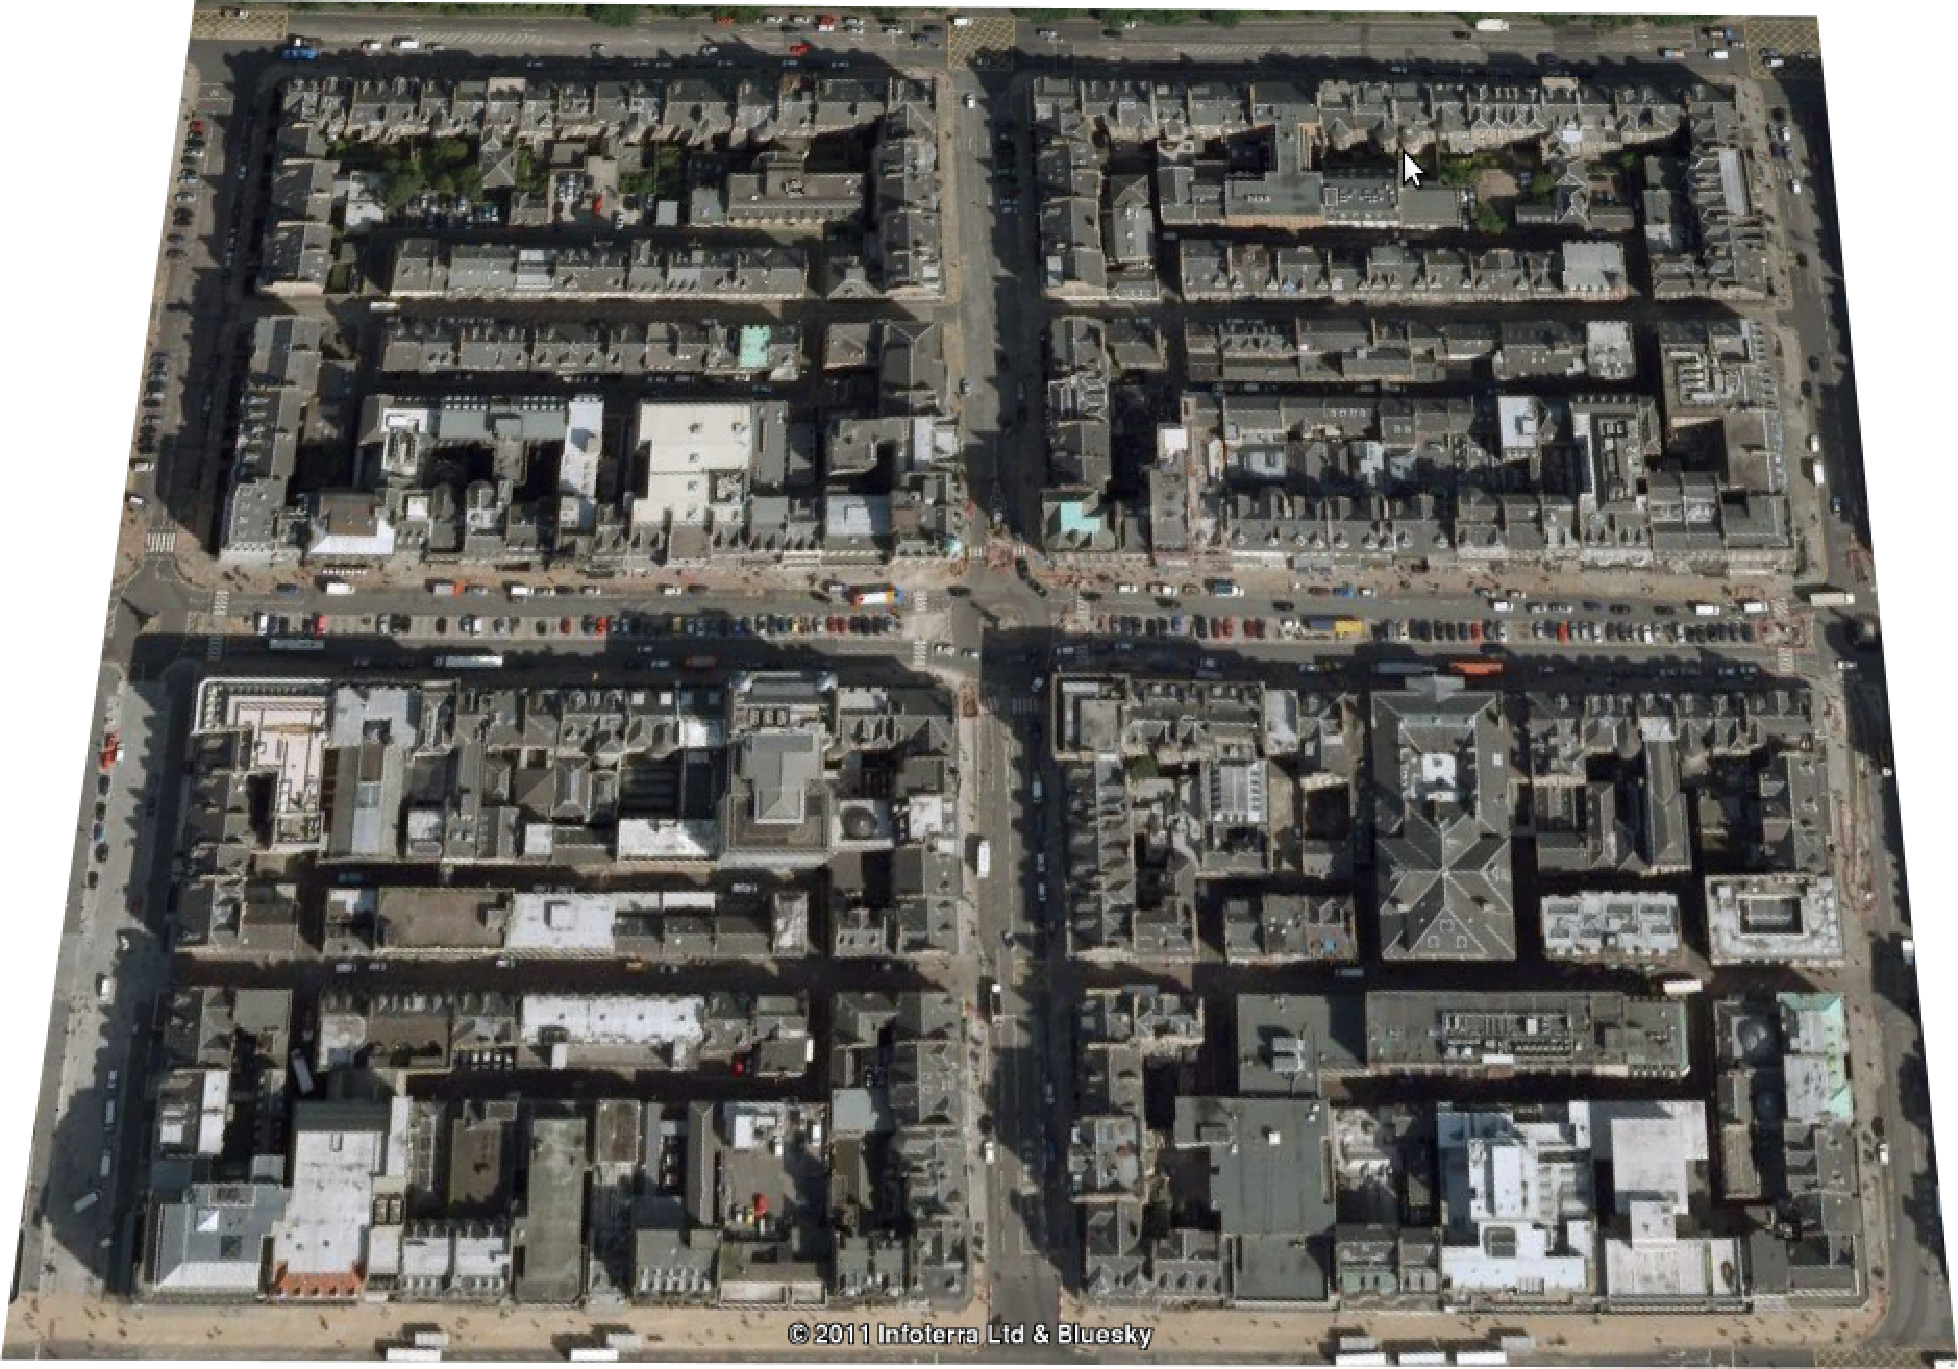
\includegraphics[width=0.8\linewidth]{fig/edinburgh.pdf} \\
Edinburgh, city centre. \\ 
$ 55^{\circ}57 ^{\backprime}16 ^{\backprime \backprime}  N  3^{\circ} 11 ^{\backprime} 58 ^{\backprime \backprime}  W $ \\
Elevation: $66 m$ \\
Area: $\approx 400 \times 300 m $
%%%%%%%%%%%%%%%%%%%%%%%%%%%%%%%%%%%%%%%%
\column{.1\textwidth}
\textit{... 1300 km away ...}
%%%%%%%%%%%%%%%%%%%%%%%%%%%%%%%%%%%%%%%%
\column{.43\textwidth}
\centering
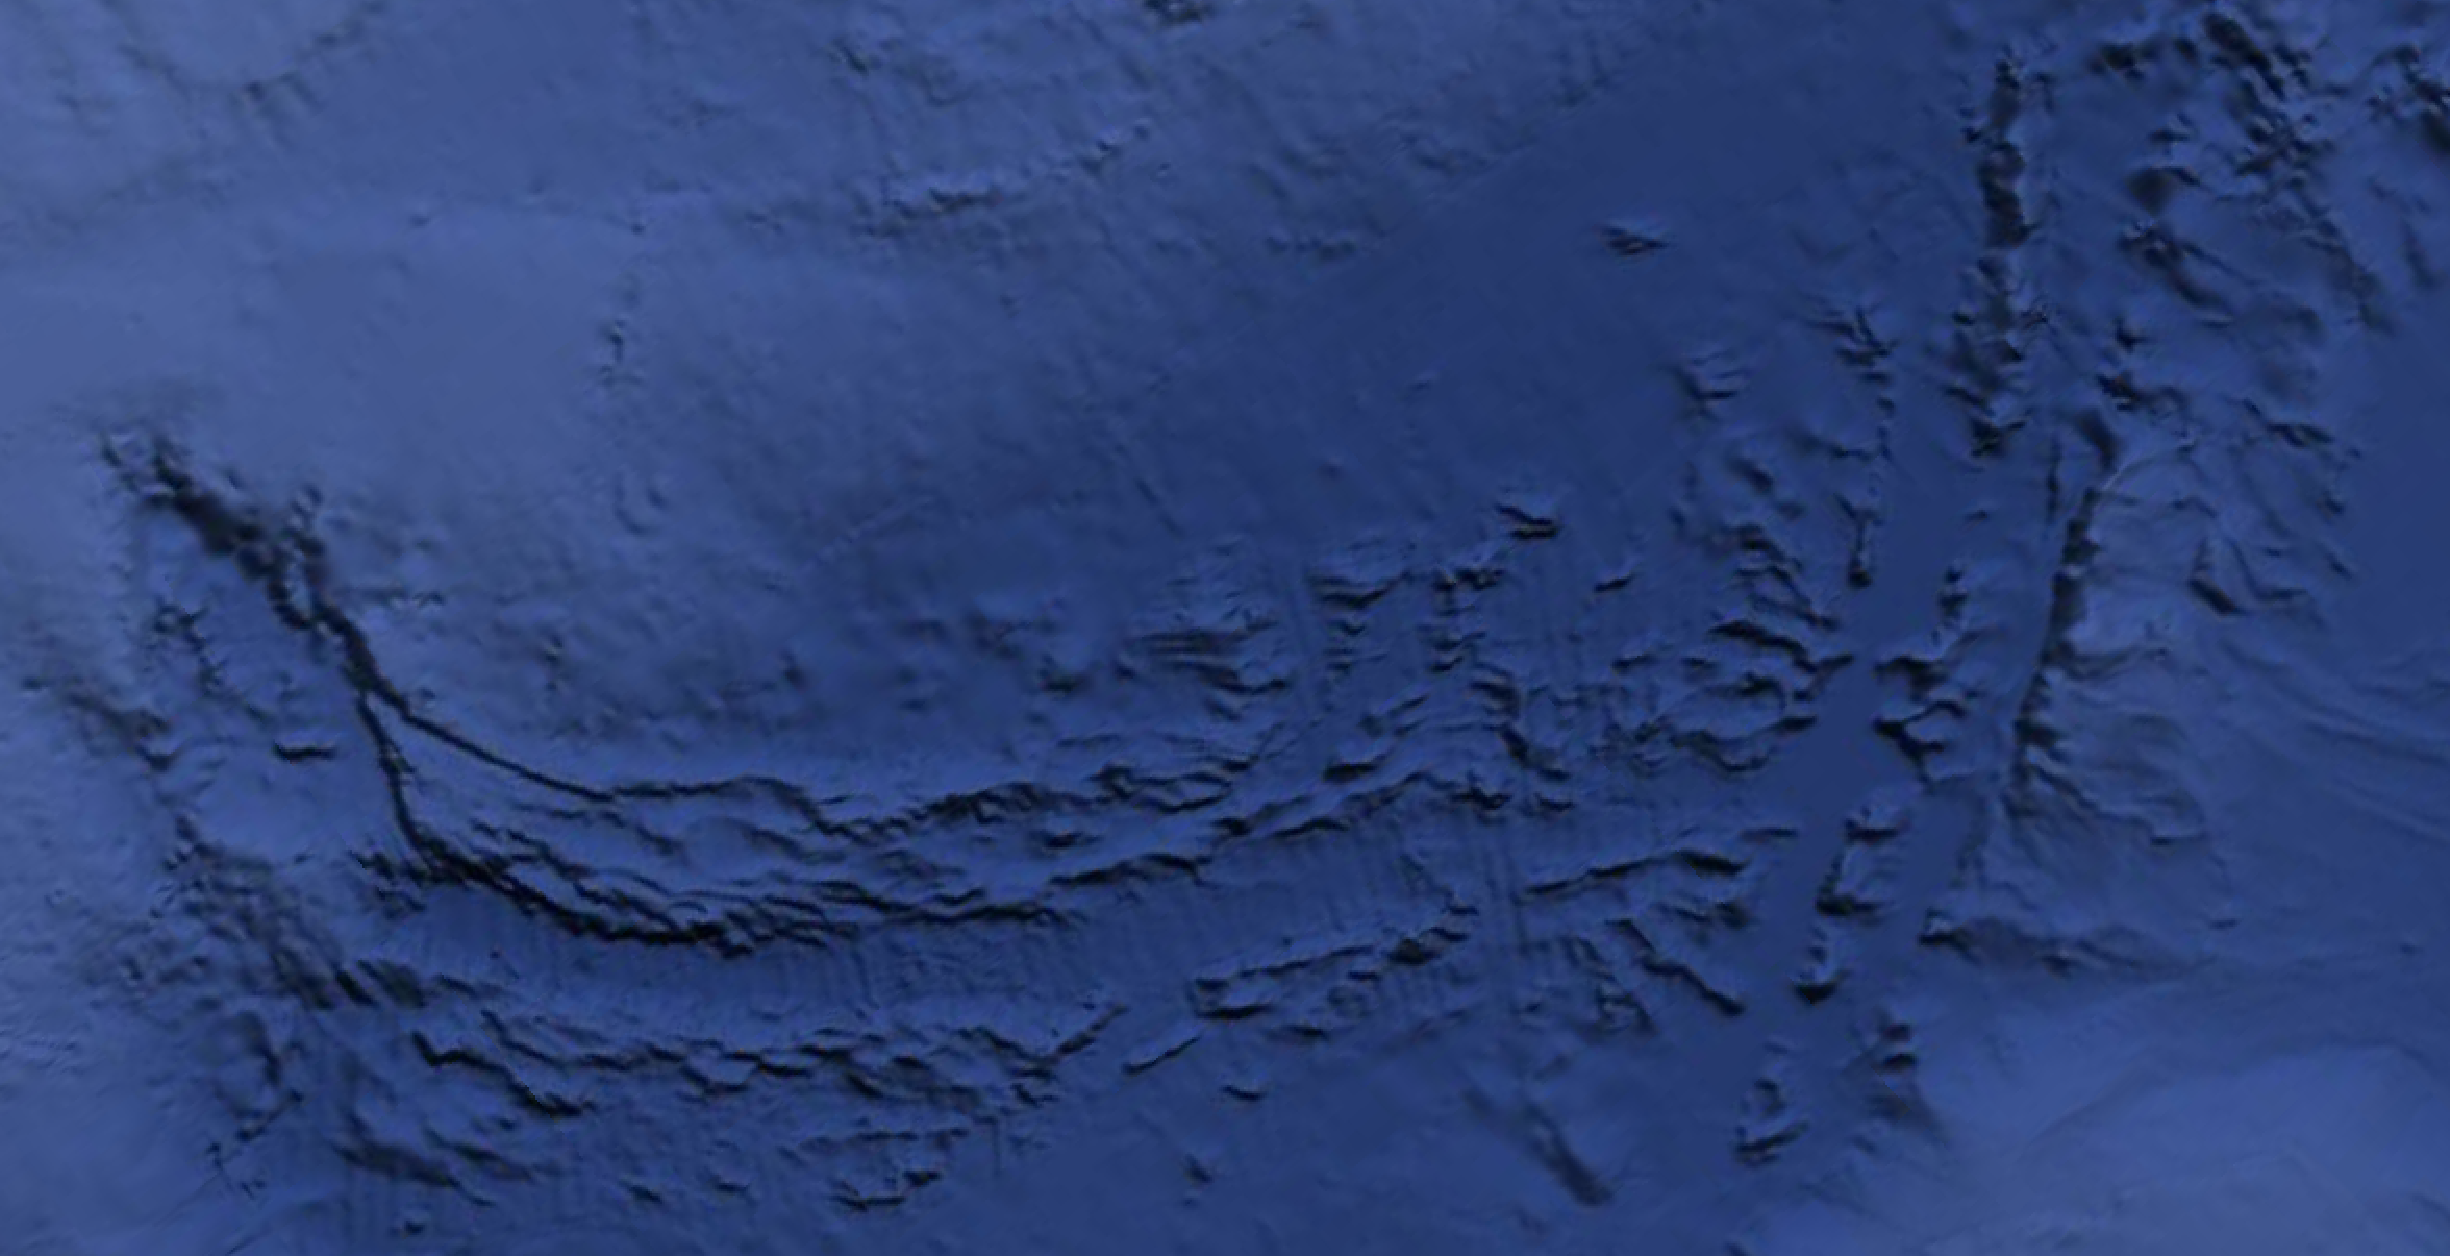
\includegraphics[width=0.8\linewidth]{fig/norwegianSea.pdf} \\
Norwegian sea. \\
$ 66^{\circ}  52 ^{\backprime} 46 ^{\backprime \backprime} N  3^{\circ}  36 ^{\backprime}  21 ^{\backprime \backprime} W $ \\
Elevation: $-3335 m$ \\
Area: $ \approx 700 \times 300 km $
\end{columns}
\end{block}

\begin{block} {Why navigation?}
	To be able to navigate the robot within the environment - we need to know it's position - to \textbf{localise} it.
\end{block}
%%mention applications: exploration, special tasks, mapping, inspections, military
\end{frame}

%%%%%%%%%%%%%%%%%%%%%%%%%%%%%%%%%%%%%%%%%%%%%%%%%%%%%%%%%%%%%%%%%%%%%%%%%%%%%%%

\begin{frame} \frametitle{Navigation}
\vspace{-10pt}
\textit{\textbf{Navigation}} implies the capabilities of:

{\footnotesize $\bullet$ accurate determination of the vehicle position and velocity with respect to a known reference point}

{\footnotesize $\bullet$ planning and the execution of the movements between locations}
\vspace{5pt}
\begin{columns}
\column{.4\textwidth}
\centering
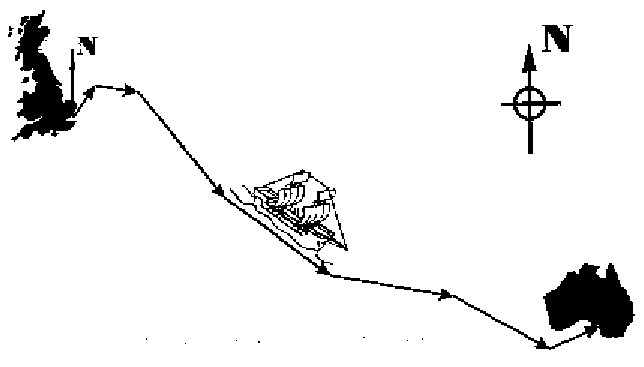
\includegraphics[width=0.8\linewidth]{fig/map.pdf} \\
{\scriptsize John Harrison, $18^{th}$ century \\
\textit{longitude problem} }


\column{.2\textwidth}
\centering
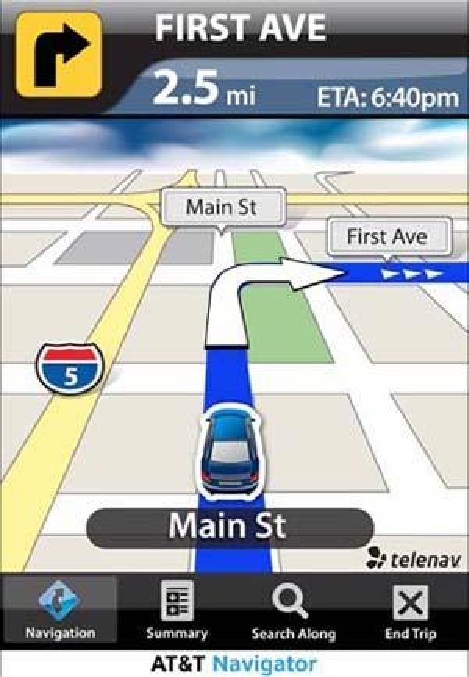
\includegraphics[height=5em]{fig/phone-navigation.pdf} \\
{\scriptsize GPS, USDOD, 1974-1994. }

\column{.3\textwidth}
\centering
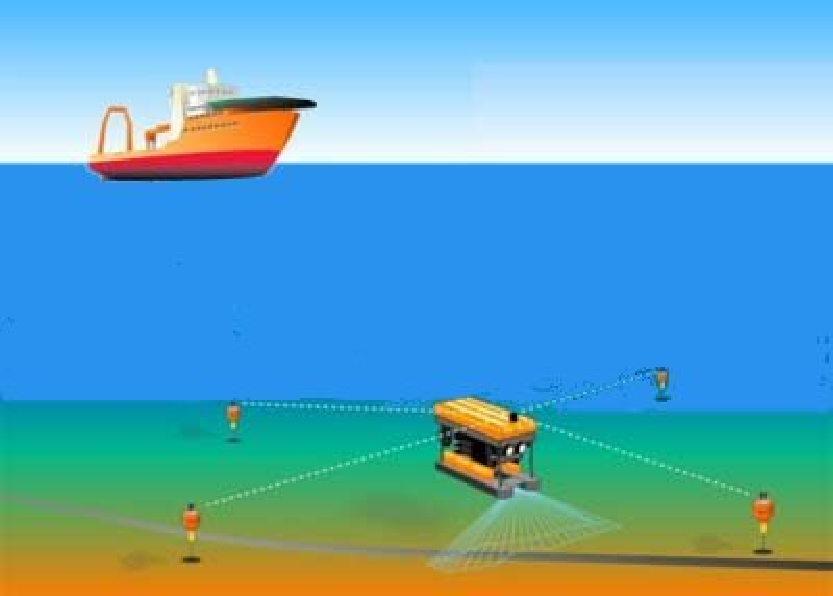
\includegraphics[height=5em]{fig/rov-navigation.pdf} \\
{\scriptsize  Underwater navigation strategies }
\end{columns} 
\vspace{5pt}
\hspace{0.5cm} \pro Measured depth is fairly accurate $\rightarrow$ localisation mainly 2d

\hspace{0.5cm} \contra Obtaining absolute position is more complex underwater

\hspace{0.5cm} \contra Cameras and sonar are of a limited use

\hspace{0.5cm} \contra Dead-reckoning sensors are expensive and prone to drifting

{\centering 
$\Longrightarrow$ use all available inertial information to navigate
}
\end{frame}

%%%%%%%%%%%%%%%%%%%%%%%%%%%%%%%%%%%%%%%%%%%%%%%%%%%%%%%%%%%%%%%%%%%%%%%%%%%%%%%

\chapter{Navigation sensors} \label{chap:sensors}
This chapter gives an overview of the sensors used for localisation of an underwater vehicle and their characteristics. Underwater positioning can be based on usage of different types of sensors combined together in one system. The role of these sensors is to measure absolute position, velocities and heading/orientation. Localization is influenced with the development and performance of sensor devices. Sensors can be regarded as the means for managing the localization. Faster they are, more accurate they are, localization has more chances to perform better. Each sensor has its own reference system in which it operates. It is important to say that sensors output measurements with reference either in body frame (Figure ~\ref{fig:auv-axes}) - the one fixed to the object or in global frame (Figure ~\ref{fig:auv-positioning}). Basic navigation sensor set for a high-end AUV usually consists of depth sensor, magnetic compass, GPS device, LBL acoustic device, Doppler Velocity Log (DVL) and gyroscope, particularly fibre-optic gyroscope (FOG).   
\section{Inertial navigation system (INS)} \label{sec:ins}
Inertial navigation combines measurements of accelerometers and gyroscopes to track down the position and orientation of an object. Motion and rotation information obtained this way are processed in order to provide an estimate of objects location with respect to  initial reference. Recent INS configurations tend to consist of compact, more accurate and higher performance sensor devices.  
\subsection{Gyroscope}
Gyroscope is an INS sensor device that essentially measures orientation of the device. Although classic gyroscope measures orientation, modern gyroscopes are capable of measuring the angular rate. Gyroscopes can be mechanical, optical or MEMS gyroscopes. Underwater navigation uses fibre-optic gyroscope (FOG). FOG is based on measuring the interference of two light beams that pass through a coiled optical fibre in both directions. FOG provides quite precise information on rotation and its usage is intended for applications that demand higher performance. 
FOG can provide the angular information: rate of change of heading (yaw rate) and the yaw/heading itself. Both measurements can be used, depending on configuration. Since the sensor actually measures yaw rate (absolute measurement), yaw can be derived by integrating yaw rate in time. Disadvantage of such principally precise measurement, is that it is relative to previous yaw value and if that value turned out to be imprecise, drift can increase or contain a permanent bias. The KVH DSP-3000 device provides the Nessie vehicle with accurate angular rates.
\subsection{Doppler Velocity Log (DVL)}
DVL is intended to measure  velocities. Transceiver components mounted on the device, pointing downwards (towards the bottom) emit acoustic impulses which are expected to be reflected if the DVL is close enough to the bottom. In case of existing reflectance it is called having ``bottom-lock''. DVL usually has four transceivers. Each of them makes an angle with respect to the sea floor. If ``bottom-locked'', those four sensors undergo Doppler shift effect. Besides Doppler speeds, DVL measures roll, pitch and heading angles and fuses them together when computing surge, sway and heave velocity within the 3D speed vector in world referenced frame. The Teledyne Explorer PA DVL is used on Nessie AUV. This unit supplies the vehicle with altitude, surge, sway and heave velocities. Operation altitude ranges from 0.5 m to 80 m. Accuracy of the measured speeds is 0.7 cm/s when moving at the speed of 1 m/s.

\subsection{Magnetic compass} 
Magnetic compass provides 3D vector of local magnetic field. Magnetic compass points at magnetic north. Direction is determined so that it aligns with Earth's magnetic field. Important procedure before starting the compass usage is calibration. North direction as it appears on maps points to the geographic north (``true north''). That is the direction towards the rotation axis of the Earth. The direction of the \textit{magnetic north} does not overlap with the direction of the geographic north. Magnetic declination is an angle between magnetic north (measured by compass) direction and the true north direction (the one that maps refer to). Depending on location where the compass is used, magnetic declination can vary and the variation is different on different spots on the Earth's surface. Hence the calibration is necessary before usage. Magnetic compass gives measurements with slow variation in space. In addition, different magnetic effects caused by electric currents can affect the measurement, thus it is robust absolute measurement of heading, nonetheless, prone to noise. Nessie vehicle uses TCM 2.6 compass that precisely measures heading, pitch, and roll. Accuracy of the heading measurement is $0.8^{\circ}$.
\subsection{Depth sensor} 
Bathymetry system accomplishes depth measurement. It is possible to use the acoustic system for this purpose, however, bathymeter using pressure information tends to be more precise and trustable. Pressure sensor is standard piece of the equipment for an AUV. By measuring the pressure, it becomes possible to correlate the value of pressure with the value of depth. Device can frequently ascertain the absolute depth with good precision. A Keller Series 33X depth sensor measures the distance to surface having the depth range of 0 - 90 m and the accuracy of 0.05 m. 
\subsection{Global Positioning System (GPS)}
This well known satellite-based navigation system provides position information anywhere on the Earth surface or in the air, reasonably close to the surface. Due to absorption of electromagnetic waves in the water GPS signal is not available underwater. Despite the fact that GPS is not available, vehicles are equipped with GPS receiver intended to be used for initial position information before submerging or for occasional position updates if the vehicle temporarily goes back to the surface. Precision of the GPS position information can vary. Namely, range of the standard deviation errors can have the order of 25.27 m \cite{farrell98}. Such huge deviation can cause significant inaccuracies in navigation. An example of the influence of GPS imprecision was shown in Figure ~\ref{fig:with-gps}. Differential GPS (DGPS) \cite{farrell98} can be used in situations when better precision is needed.
\section{Acoustic positioning system}
Provides the absolute position, a ground-based reference. Principal way of exchanging the information through the environment is sound wave. Long baseline (LBL) is used for measuring position with respect to several tethered beacons with known position, placed in water (Section \S~\ref{sec:acoustic}). It can be understood as the extension of the GPS information below the water surface. Such system employs acoustic signals to measure the distances. Vehicle uses the acoustic transponder to send the acoustic wave (``pinging''). The wave reaches beacon and reflects back to the vehicle . LBL system consists of transceiver and array-arranged collection of beacons. LBL transceiver pings each of the beacons and detects the signal travel time in order to calculate the distance, knowing the speed of sound in water. Distances from the beacons are combined together in triangulation method. Triangulation makes it possible to determine the position of the robot in the network of fixed beacons. LBL position update can introduce the outliers that need to be rejected or filtered. 
%As stated in some practical implementations (\cite{blain03}), DVL and acoustic sensor perform ...
\begin{figure}
  \centering
    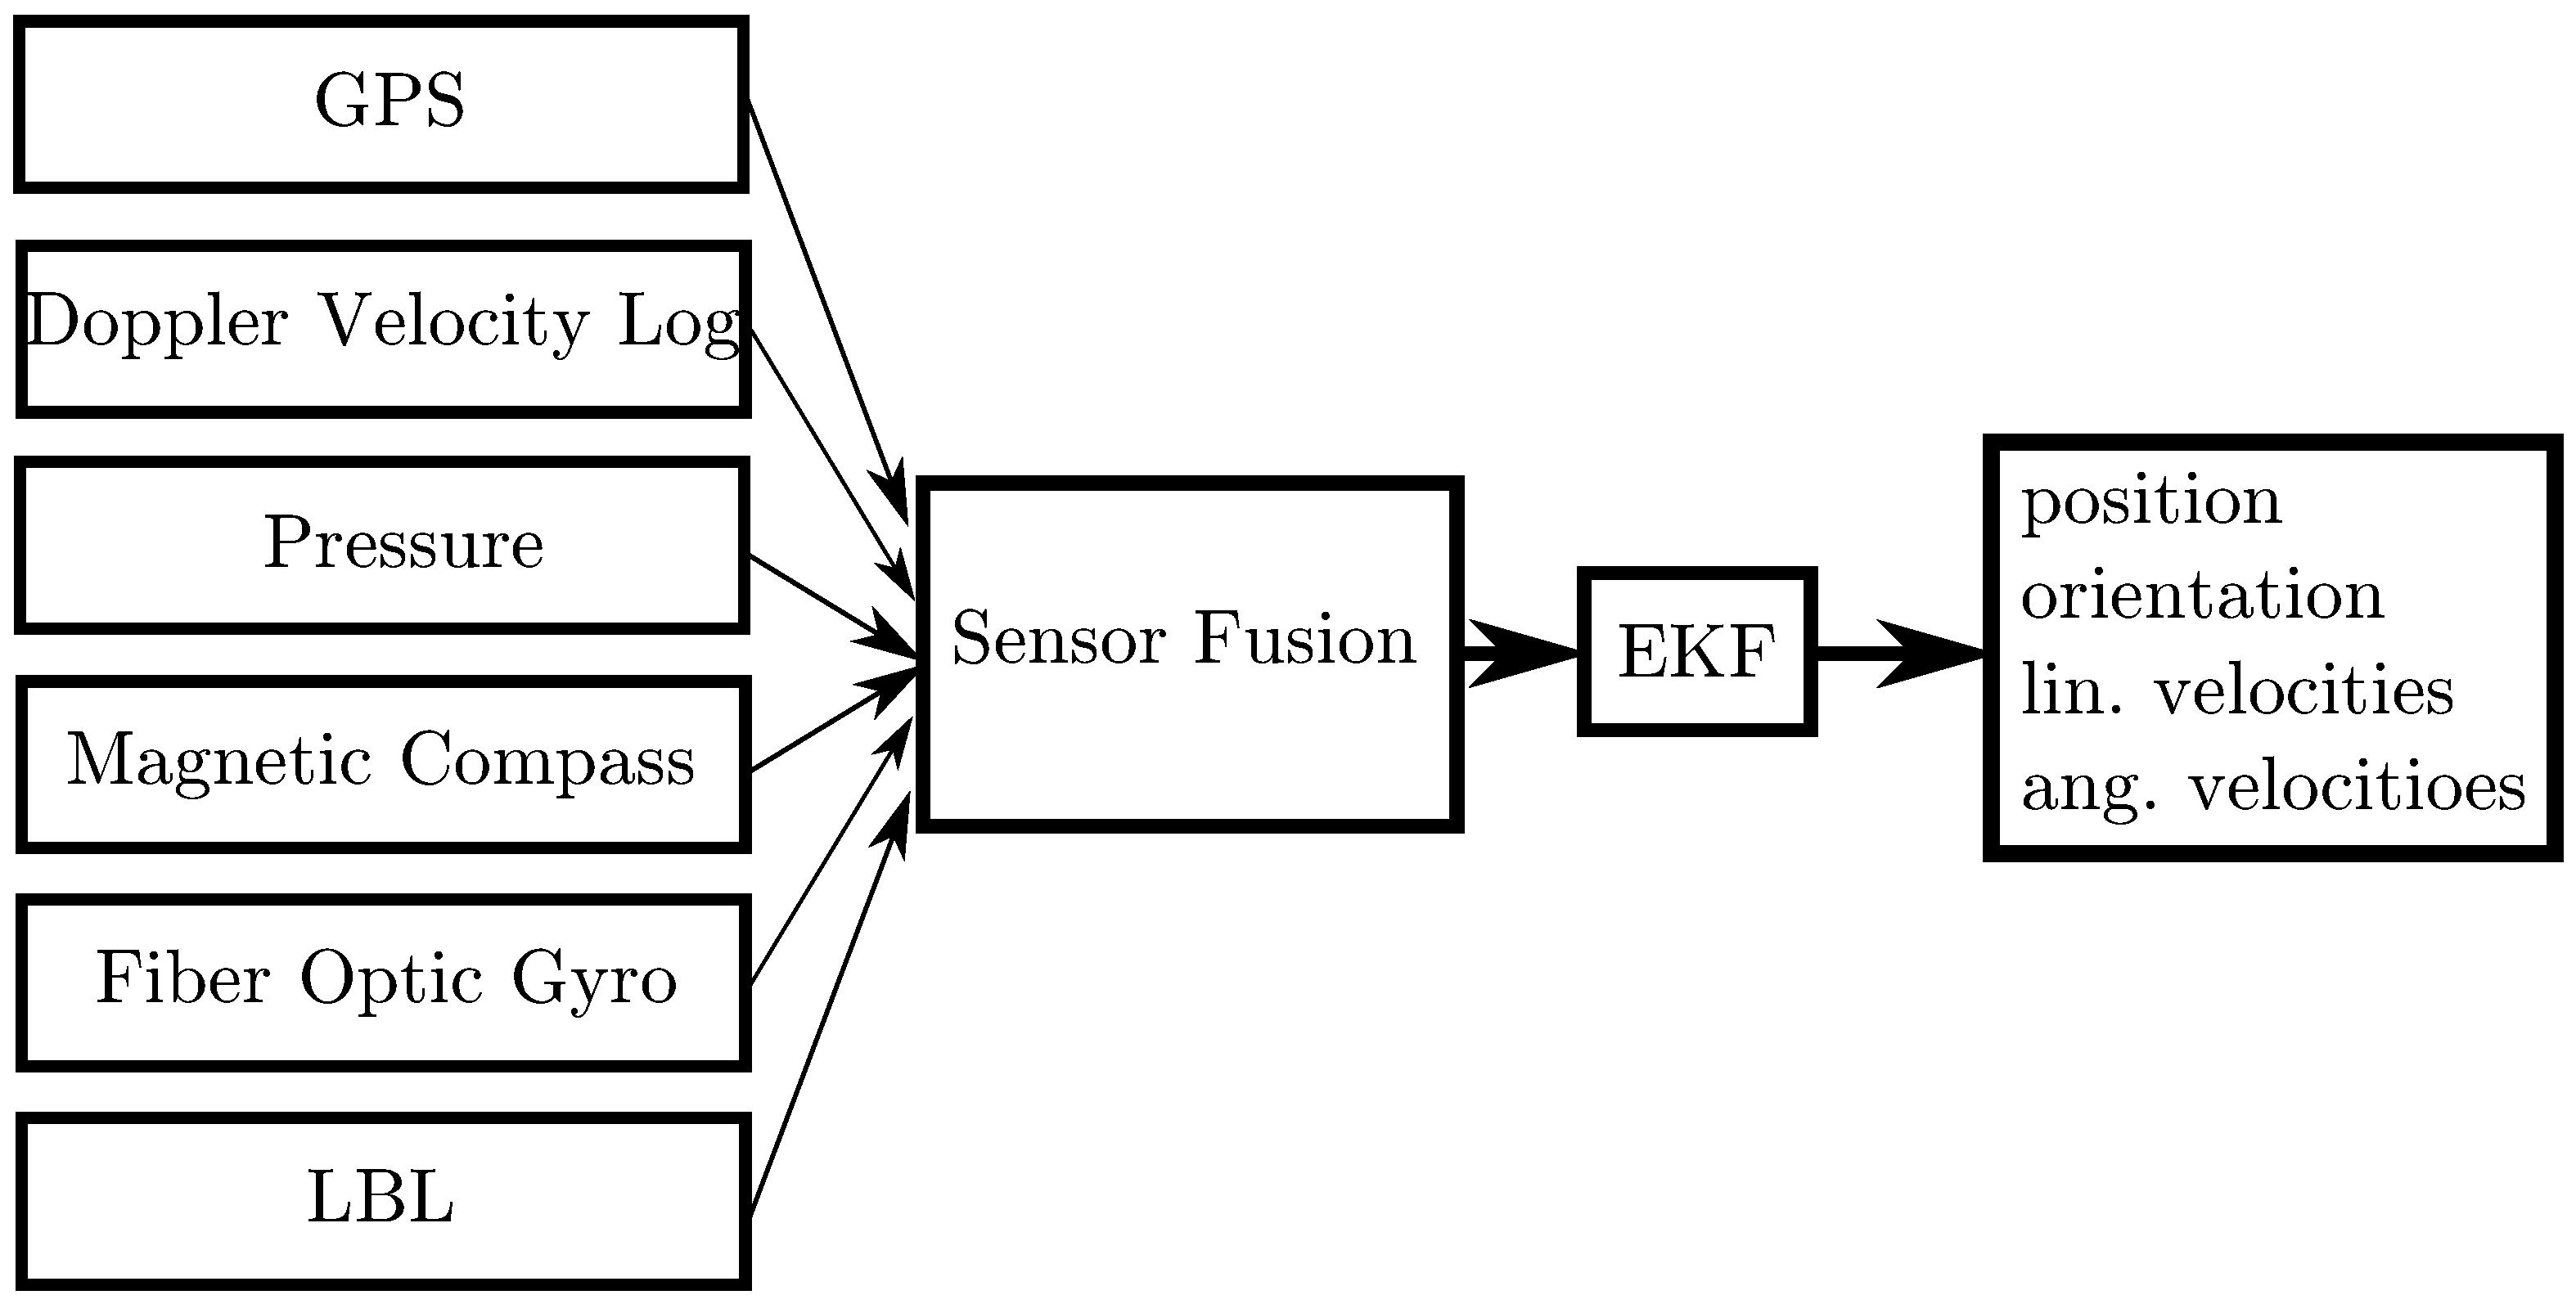
\includegraphics[width=0.65\textwidth]{methodology/fig/fusion.eps}
  \caption{Sensor fusion diagram.}
\vspace{-10pt}
\label{fig:sensor-fusion}
\end{figure}
\begin{table*}
\centering
	\caption{Navigation sensors characteristics.}
	\label{tab:sensors-char}
\begin{tabular}{llllll}
\toprule
Sensor      &     Measures     &   Update rate   &   Precision	  &    Accuracy    &    Range  \\
\midrule
\multirow{4}{*}{Pressure} & \multirow{2}{*}{depth} & \multirow{2}{*}{10 Hz} & 0.0002 $bar$ & 0.005 $bar$ & $0 - 10$ $bar$  \\
         	              &   &                         & (0.002 $m$)  &  (0.05 m)   & (0-90 $m$ in water) \\ 
                          & \multicolumn{5}{c}{\contra heave velocity is calculated by deriving depth in time - higher possibility of error} \\ 
        	              & \multicolumn{5}{c}{\pro distance from surface available no matter of distance from the seabed} \\                      
\midrule
\multirow{6}{*}{Compass}&yaw(heading)&\multirow{3}{*}{10 Hz}& $0.1^{\circ}$ & $0.8^{\circ}$ &              \\
         	            &pitch       &                       &               &               & tilt $\pm 50 ^{\circ}$  \\
         	            &roll        &                       &                &                &                    \\
  & \multicolumn{5}{c}{\pro absolute measure of heading - no drift } \\
  & \multicolumn{5}{c}{\contra needs magnetic north correction (due to magnetic declination)} \\
  & \multicolumn{5}{c}{\contra prone to magnetic disturbance} \\
\midrule
\multirow{2}{*}{FOG} & \multirow{2}{*}{yaw rate} & \multirow{2}{*}{5Hz} & \multirow{2}{*}{$ < 1^{\circ} / hr$} & \multirow{2}{*}{$\pm 20^{\circ} / hr$} & \multirow{2}{*}{$\pm 375 ^{\circ}/s$} \\
     &          &           &           &         &         \\
 & \multicolumn{5}{c}{\pro high accuracy in heading measurement, compared to compass} \\
 & \multicolumn{5}{c}{\contra drifts over time, needs correction for the Earth rotation} \\
\midrule
\multirow{3}{*}{DVL} & surge velocity & \multirow{3}{*}{10 Hz} & \multirow{3}{*}{$0.1\frac{cm}{s}$} & $ \pm 0.7\frac{cm}{s}$ at $1\frac{m}{s^{4}}$ & \multirow{3}{*}{$\pm 9.5\frac{m}{s}$} \\
         	        &sway velocity&                        &                                    & $ \pm 1.9\frac{cm}{s}$ at $3\frac{m}{s^{4}}$ &                                  \\
         	        &heave velocity &                      &                                    & $ \pm 3.0\frac{cm}{s}$ at $5\frac{m}{s^{4}}$ &                              \\
 & \multicolumn{5}{c}{\contra relative measurement of velocity} \\
 & \multicolumn{5}{c}{\contra requires depth - looses lock at $0.6$ $m$ altitude resulting in no output} \\
\bottomrule
\end{tabular} 
\end{table*}

%%%%%%%%%%%%%%%%%%%%%%%%%%%%%%%%%%%%%%%%%%%%%%%%%%%%%%%%%%%%%%%%%%%%%%%%%%%%%%%

\begin{frame}\frametitle{Vehicle Navigation State Vector}
%The aim: accurate determination of the vehicle position and velocity
\begin{columns}
	\column{.62\textwidth}
	\textit{Vehicle state} is a vector that contains variables relevant for localising the vehicle (Eq. ~\ref{eq:state}). Vehicle navigation state describes its position and motion within the environment. Elements of the state vector $\vect{X}(k)$ are treated as Gaussian Random Variables (GRV). State vector will combine angular and metric values. \\
	{\footnotesize
	\begin{align}
		\vect{X}(k) = \left[ 
		\begin{array}{ccccccccccc}
		x & y & z & a & u & v & w & \psi & \varphi & \dot{\psi} & \dot{\varphi}
		\end{array} \right] ^{T}
		\label{eq:state}
	\end{align}
	}
{\footnotesize	
$\boldsymbol{x, y, z, a}$ : \textit{north}, \textit{east}, \textit{depth} and \textit{altitude} (Fig. \ref{fig:pos}). \\ 
$\boldsymbol{u, v, w}$ : linear velocities w.r.t sea bed in vehicle's coordinate system (\textit{surge}, \textit{sway} and \textit{heave}, Fig. \ref{fig:vel}) \\
$\boldsymbol{\psi, \varphi}$ : \textit{yaw} and \textit{pitch} (vehicle orientation, Fig. \ref{fig:pos}). \\
$\boldsymbol{\dot{\psi}, \dot{\varphi}}$ : \textit{yaw rate} and \textit{pitch rate} (angular velocities). 
} 
		
	\column{.35\textwidth}
	\begin{figure} %u, v, w - Velocity w.r.t sea bed in body coordinate
	\subfigure[velocities w.r.t. sea bed]{\label{fig:vel} 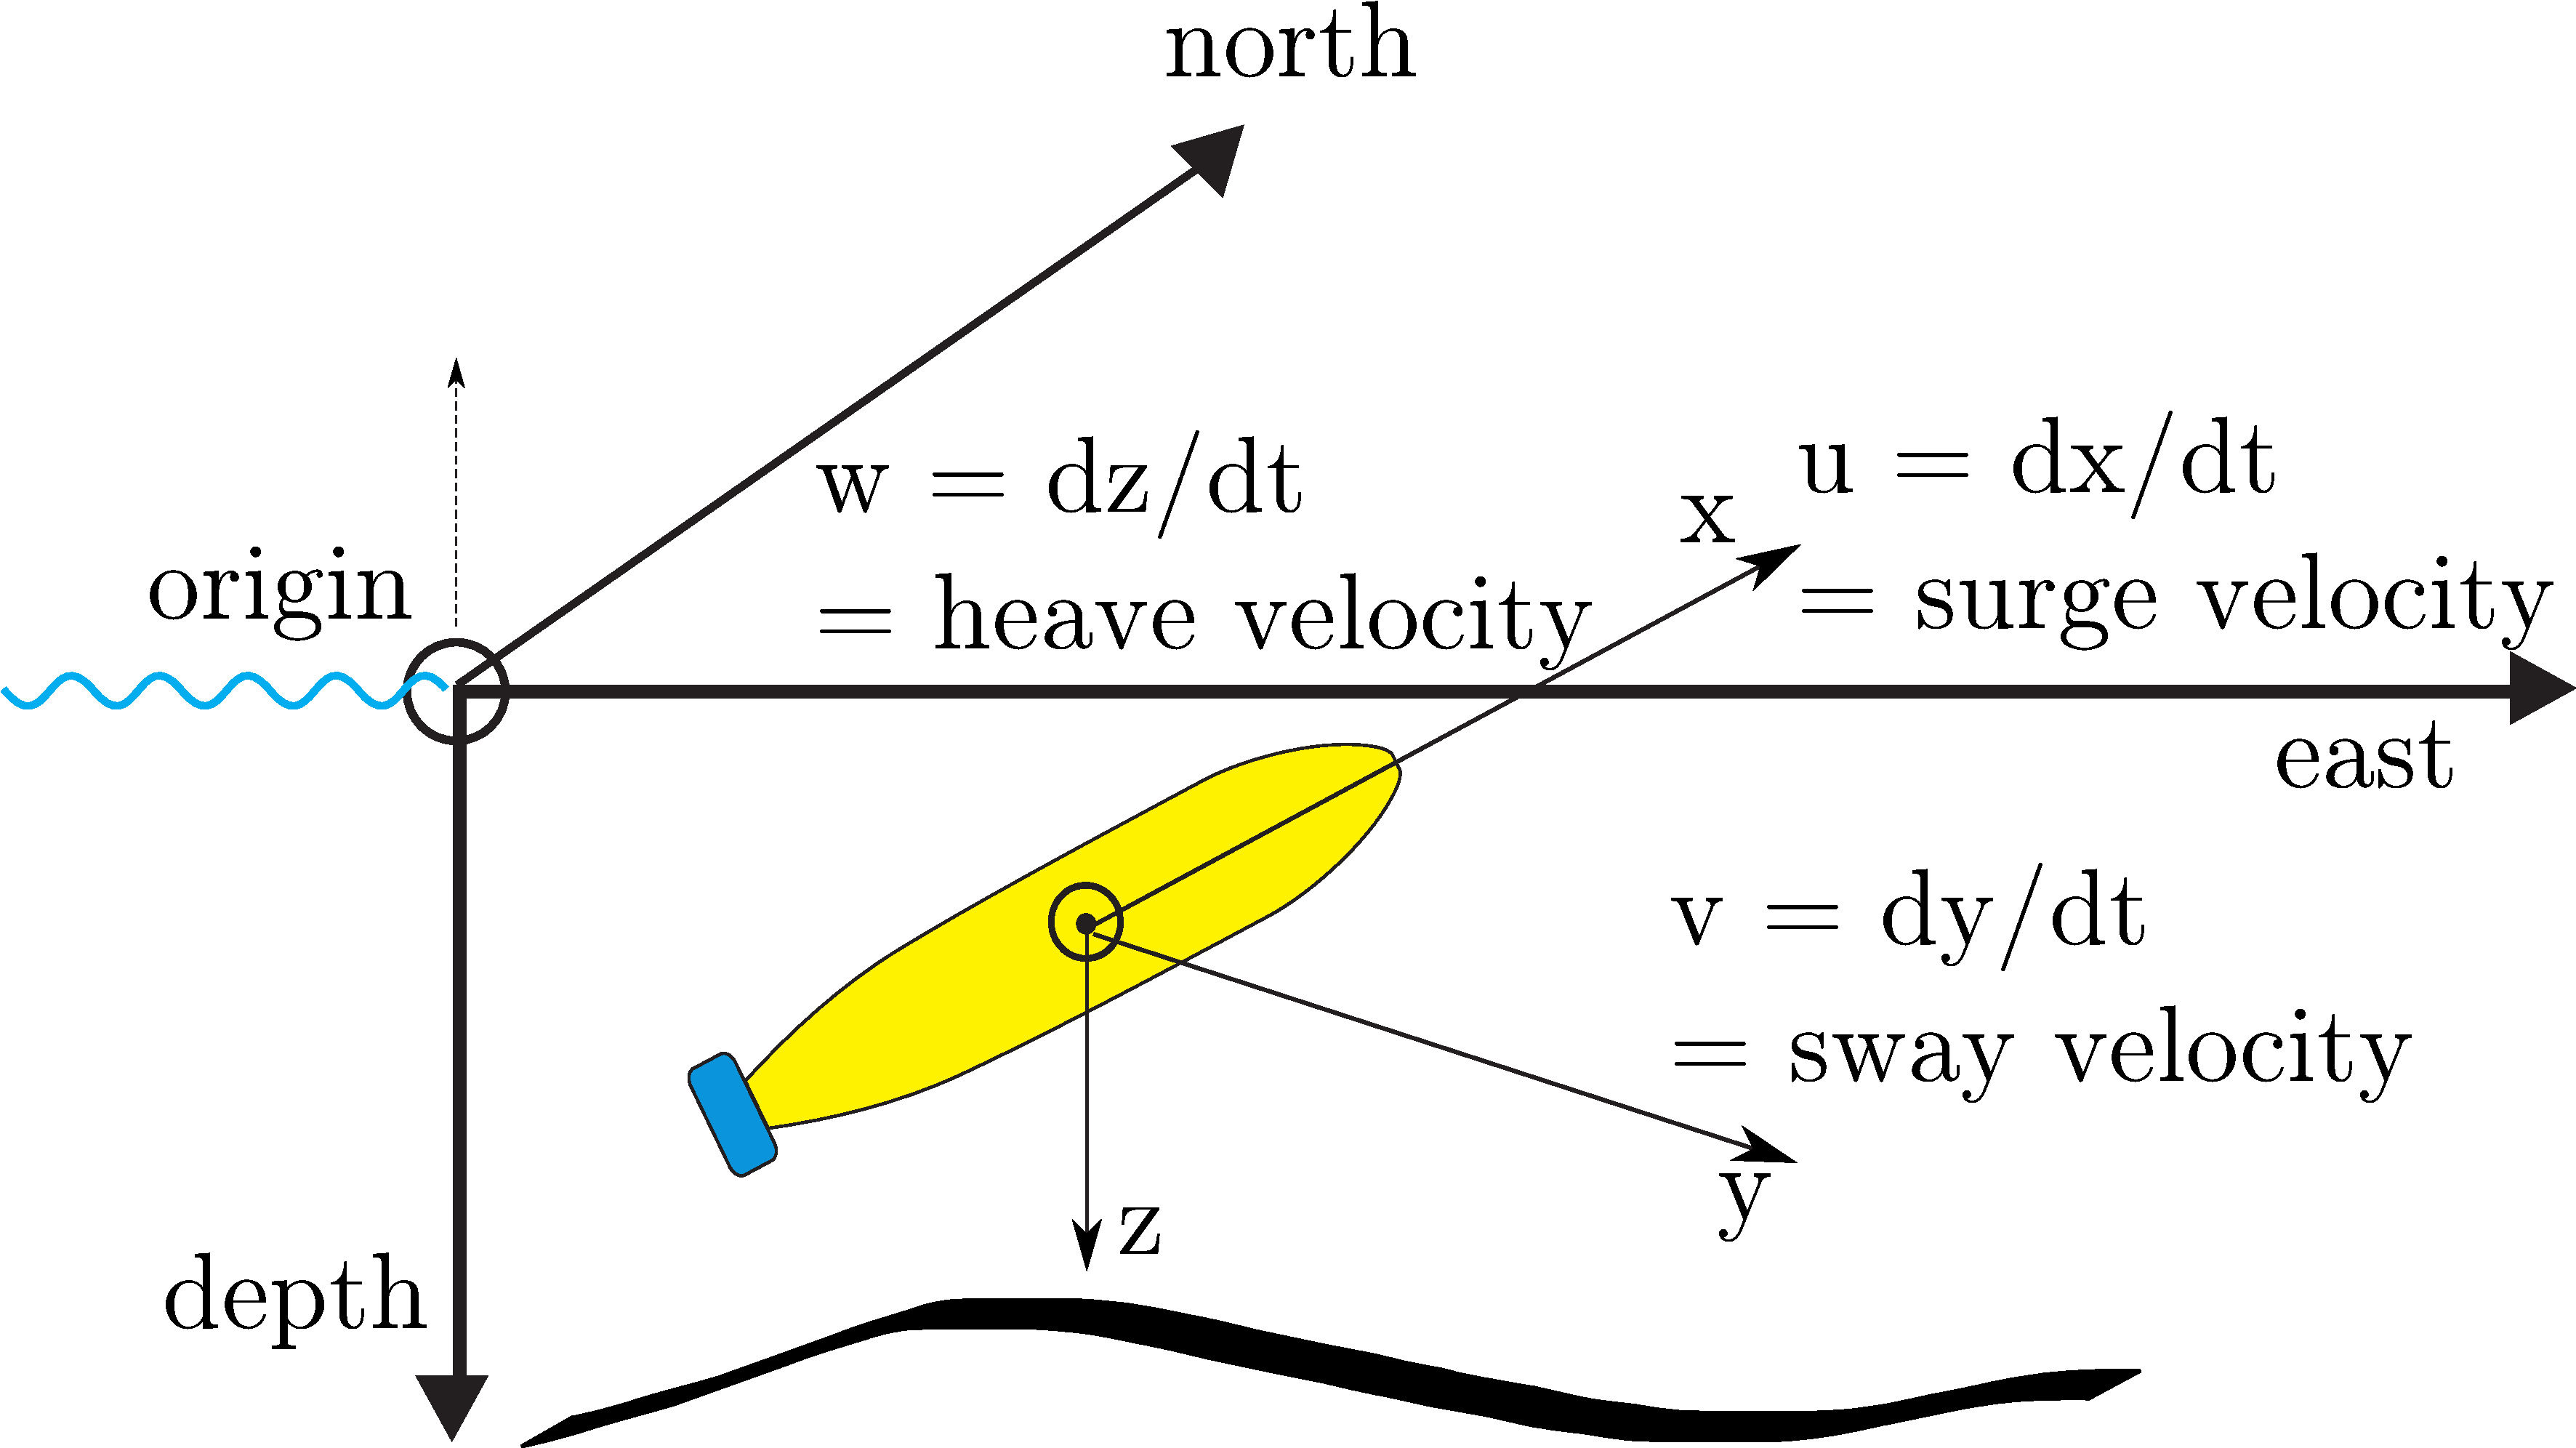
\includegraphics[width=0.95\linewidth]{fig/auv-axes.pdf}} \\
	\subfigure[global positioning]{\label{fig:pos} 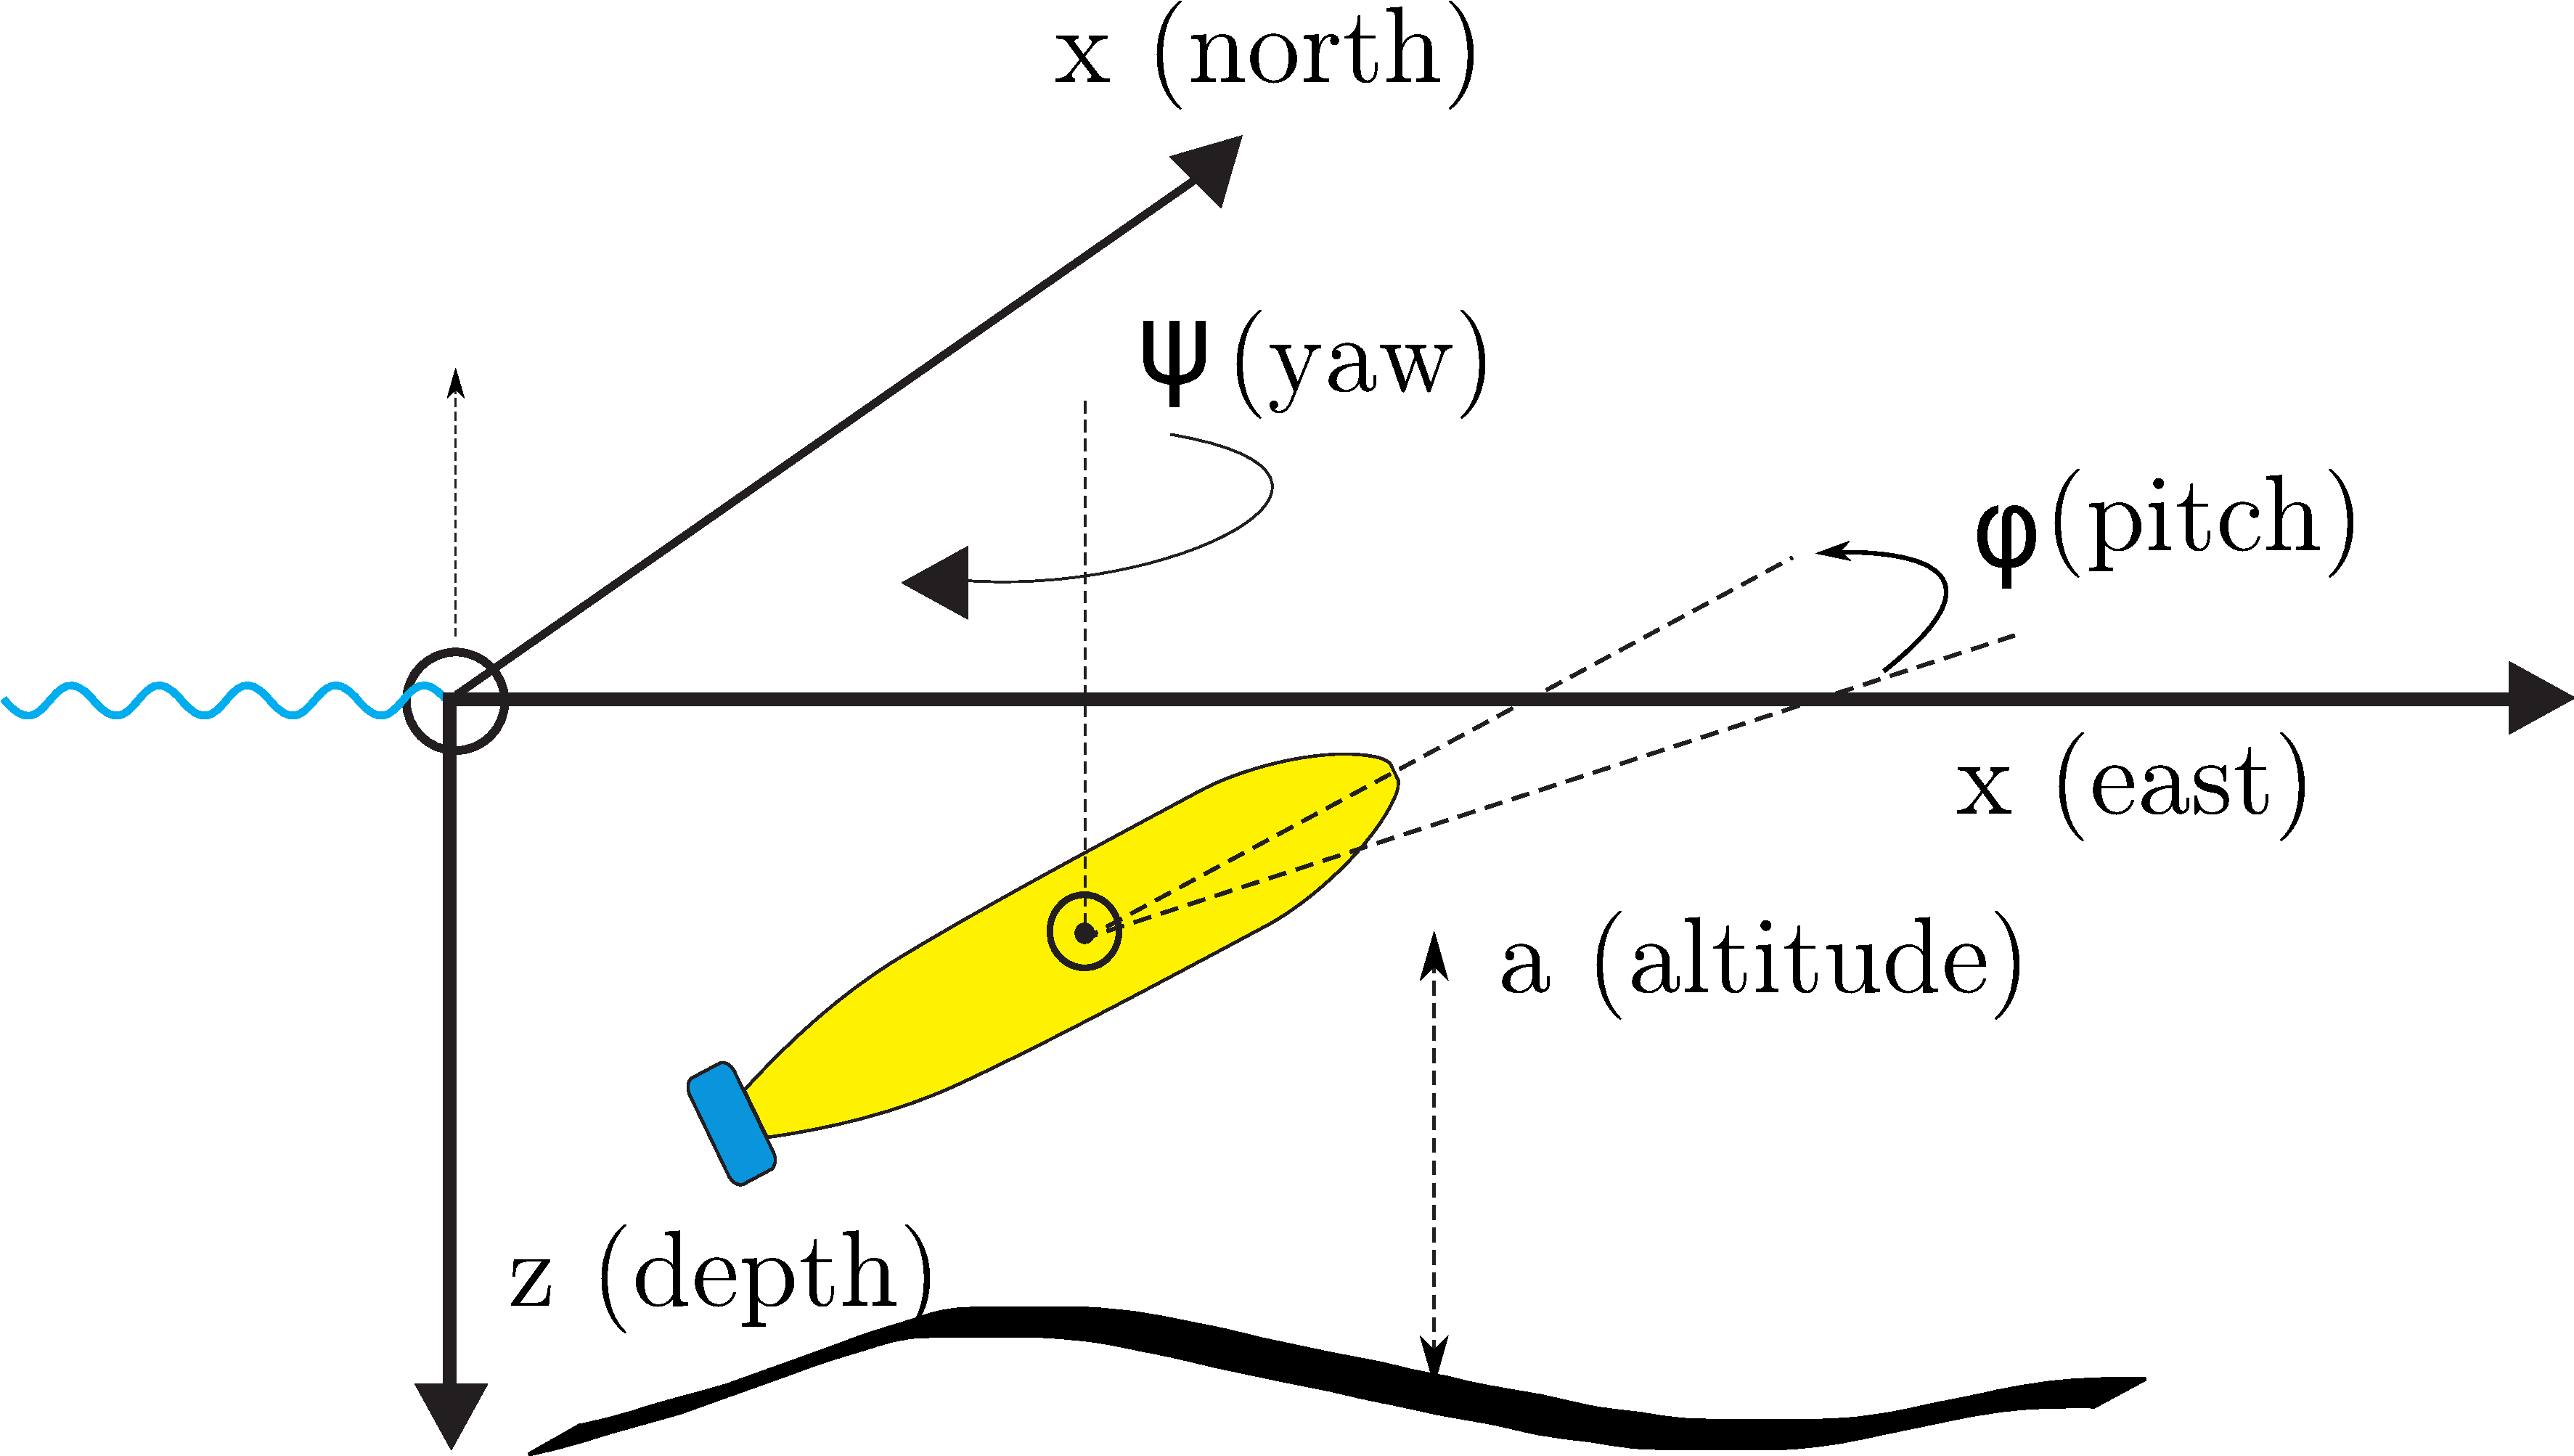
\includegraphics[width=0.95\linewidth]{fig/auv-model.pdf}}
	\caption{AUV positioning}
	\vspace{-25pt}
	\label{fig:positioning}
	\end{figure}
	
\end{columns}
\end{frame}



%%%%%%%%%%%%%%%%%%%%%%%%%%%%%%%%%%%%%%%%%%%%%%%%%%%%%%%%%%%%%%%%%%%%%%%%%%%%%%%

\begin{frame}\frametitle{System Model}
5 d.o.f. system model is describing how the state $\vect{X}(k)$ evolves in time. It is a \textit{constant speed} model \cite{ribas10} that uses previous state $\vect{X}(k-1)$ corrupted with \textit{zero-mean} GRV with linear and angular acceleration noise  $\vect{N}(k-1)$ to make a prediction of the next state vector value (Fig. ~\ref{fig:state-tran}, Eq. ~\ref{eq:state-tran}, ~\ref{eq:f}).
\begin{equation}
\vspace{-5pt}
\vect{X}(k) = f(\vect{X}(k-1), \vect{N}(k-1))
\label{eq:f}
\end{equation}
$$\vect{N}(k) = \left[ \begin{array}{ccccc} \dot{u} & \dot{v} & \dot{w} & \ddot{\psi} & \ddot{\varphi} \end{array} \right]^{T}$$% represents the process noise consisting of linear and angular accelerations.
\vspace{-10pt}
\begin{columns}
\column{.6\textwidth}
\begin{tiny}
\begin{equation}
\begin{bmatrix} x \\ y \\ z \\ a \\ \boldsymbol{u} \\ \boldsymbol{v} \\ \boldsymbol{w} \\ \psi \\ \varphi \\ \boldsymbol{\dot{\psi}} \\ \boldsymbol{\dot{\varphi}} \end{bmatrix}_{(k)} =
\begin{bmatrix} x + (uT+\dot{u}\frac{T^{2}}{2})\cos(\psi)\cos(\varphi) - (vT+\dot{v}\frac{T^{2}}{2})\sin(\psi)\cos(\varphi) \\ 
                y + (uT+\dot{u}\frac{T^{2}}{2})\sin(\psi)\cos(\varphi) + (vT+\dot{v}\frac{T^{2}}{2})\cos(\psi)\cos(\varphi) \\ 
                z + (wT+\dot{w}\frac{T^{2}}{2})\cos(\varphi) \\ 
                a - (wT+\dot{w}\frac{T^{2}}{2})\cos(\varphi) \\ 
                \boldsymbol{u} + \dot{u}T \\ 
                \boldsymbol{v} + \dot{v}T \\ 
                \boldsymbol{w} + \dot{w}T \\ 
                \psi    + \dot{\psi}T    + \ddot{\psi}   \frac{T^{2}}{2} \\ 
                \varphi + \dot{\varphi}T + \ddot{\varphi}\frac{T^{2}}{2} \\ 
                \boldsymbol{\dot{\psi}}    + \ddot{\psi}T \\ 
                \boldsymbol{\dot{\varphi}} + \ddot{\varphi}T
\end{bmatrix}_{(k-1)} 
\label{eq:state-tran}
\end{equation} %% defined as zero-mean GRV.
\end{tiny}
\column{.35\textwidth}
\begin{figure}
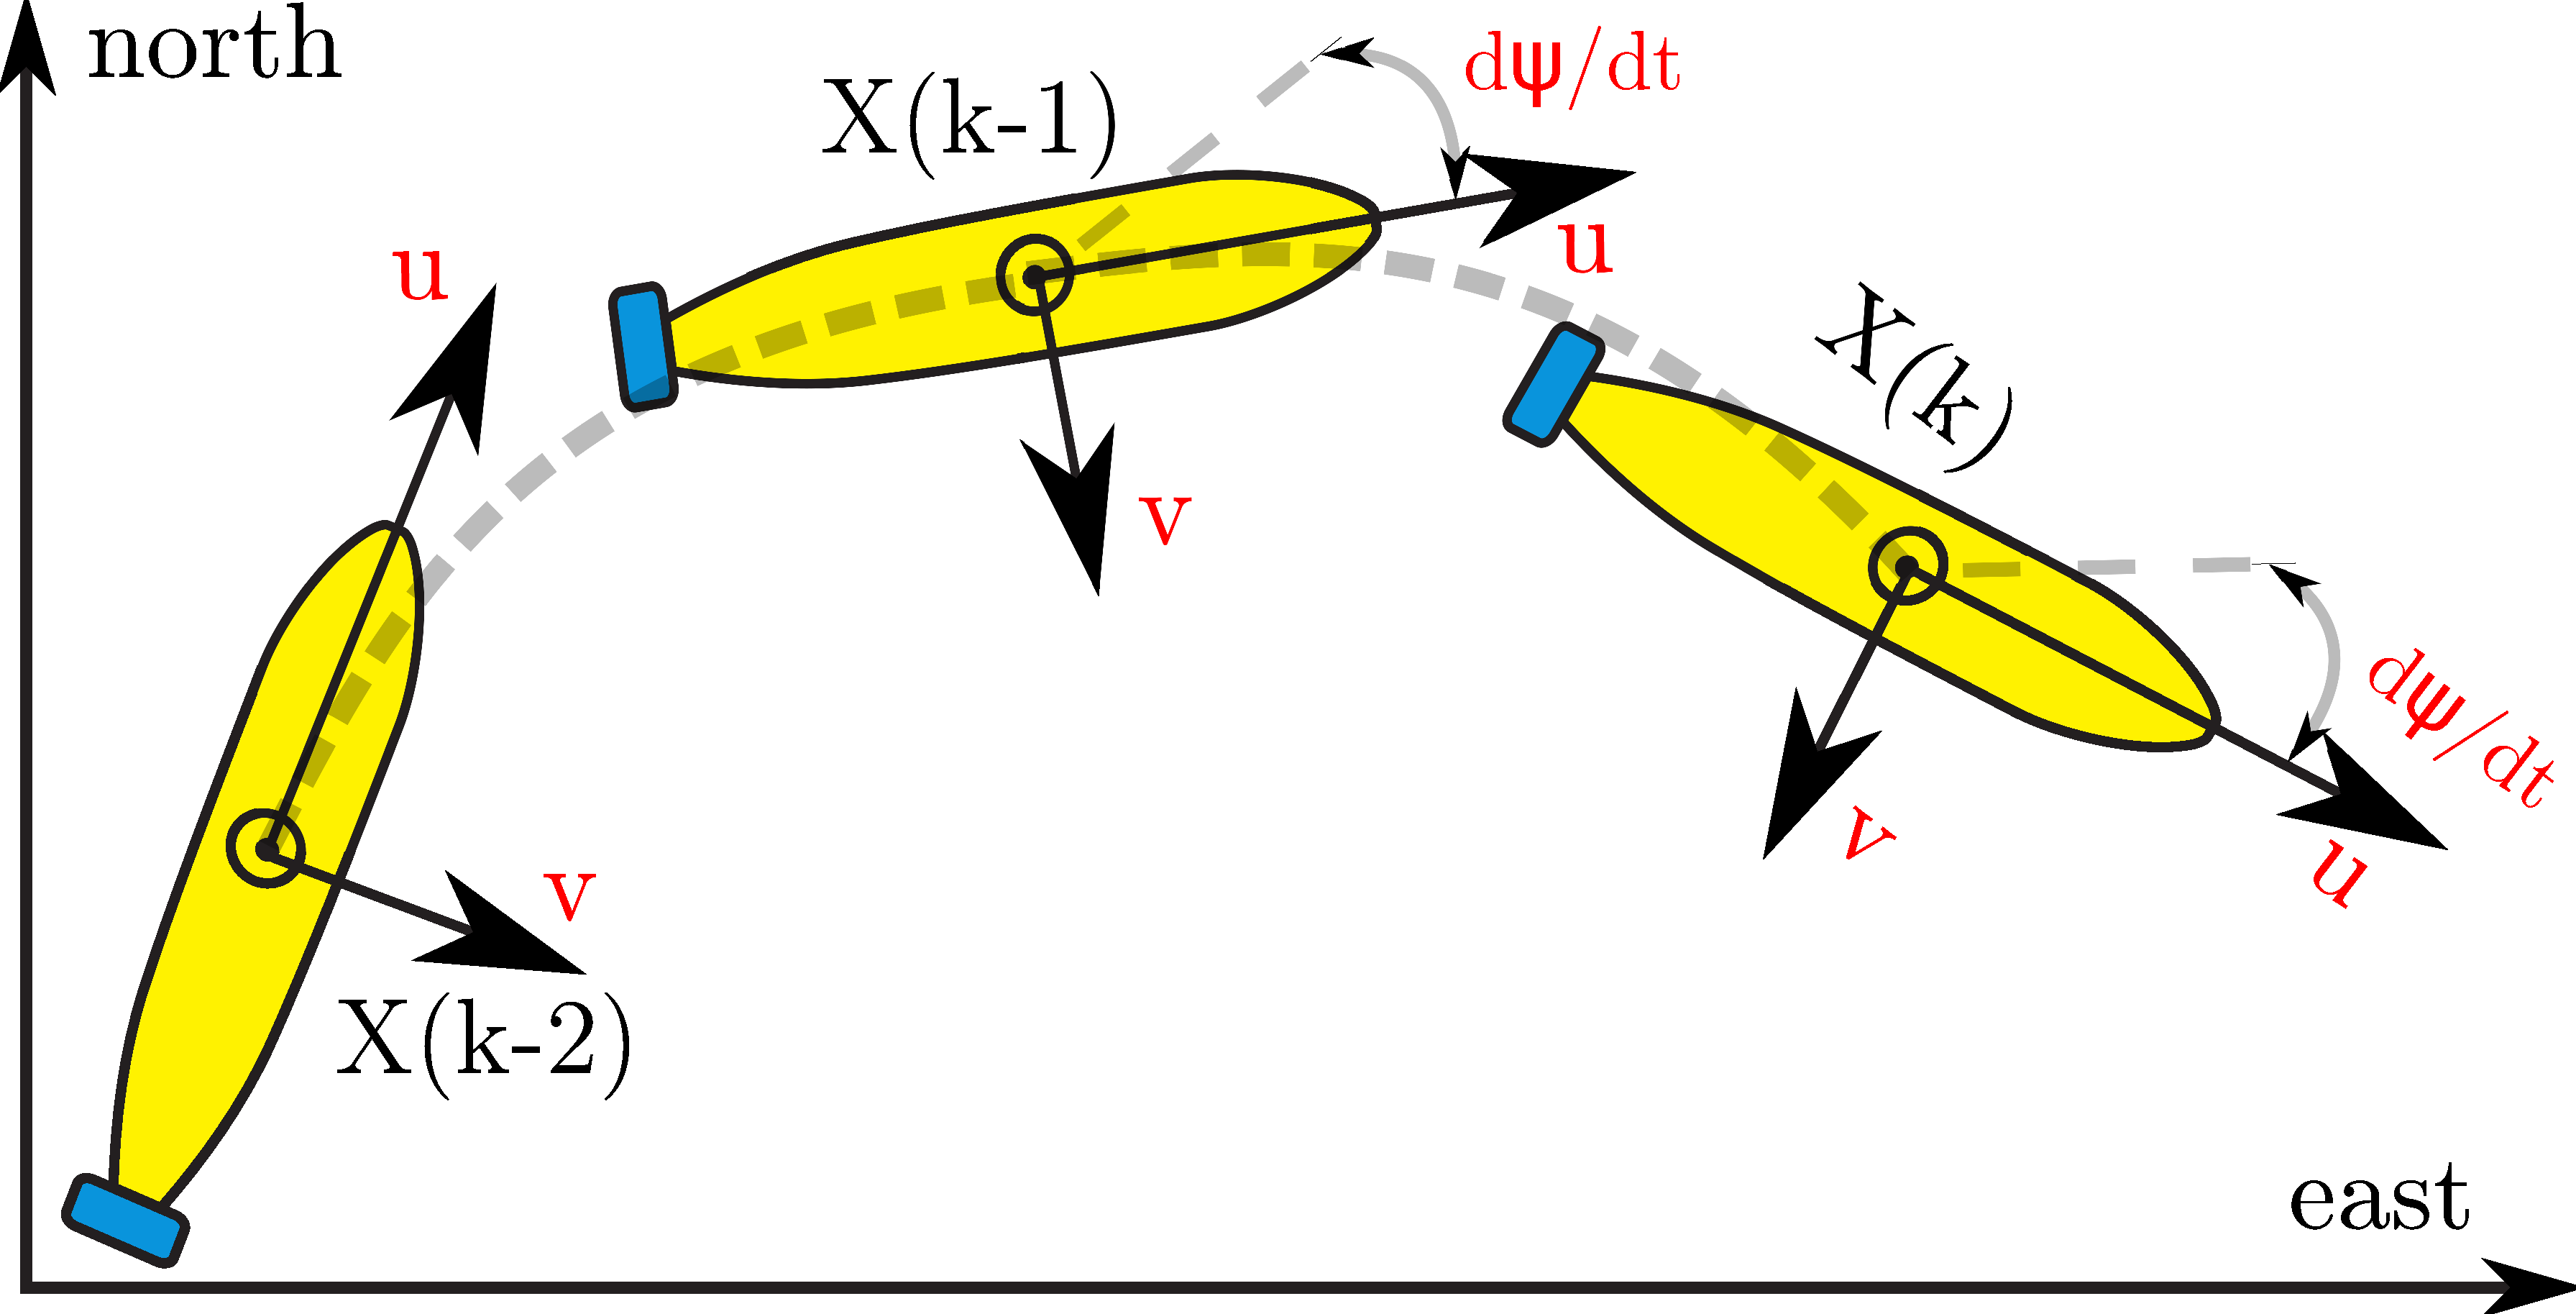
\includegraphics[width=0.98\linewidth]{fig/model.pdf}
\caption{{\scriptsize State transition model}}
\label{fig:state-tran}
\end{figure}
\end{columns}
\end{frame}

%%%%%%%%%%%%%%%%%%%%%%%%%%%%%%%%%%%%%%%%%%%%%%%%%%%%%%%%%%%%%%%%%%%%%%%%%%%%%%%

\begin{frame}\frametitle{Extended Kalman Filter (EKF)}%estimating the state of a nonlinear dynamic system
The goal is to estimate the vehicle state $\vect{X}(k)$ using sensor measurements $\vect{Z}(k)$, process $\vect{N}(k-1)$ and measurement $\vect{M}(k)$ noise. \\
\begin{columns}
	\column{.45\textwidth}
	\begin{block}{How does it work?}
	\centering
	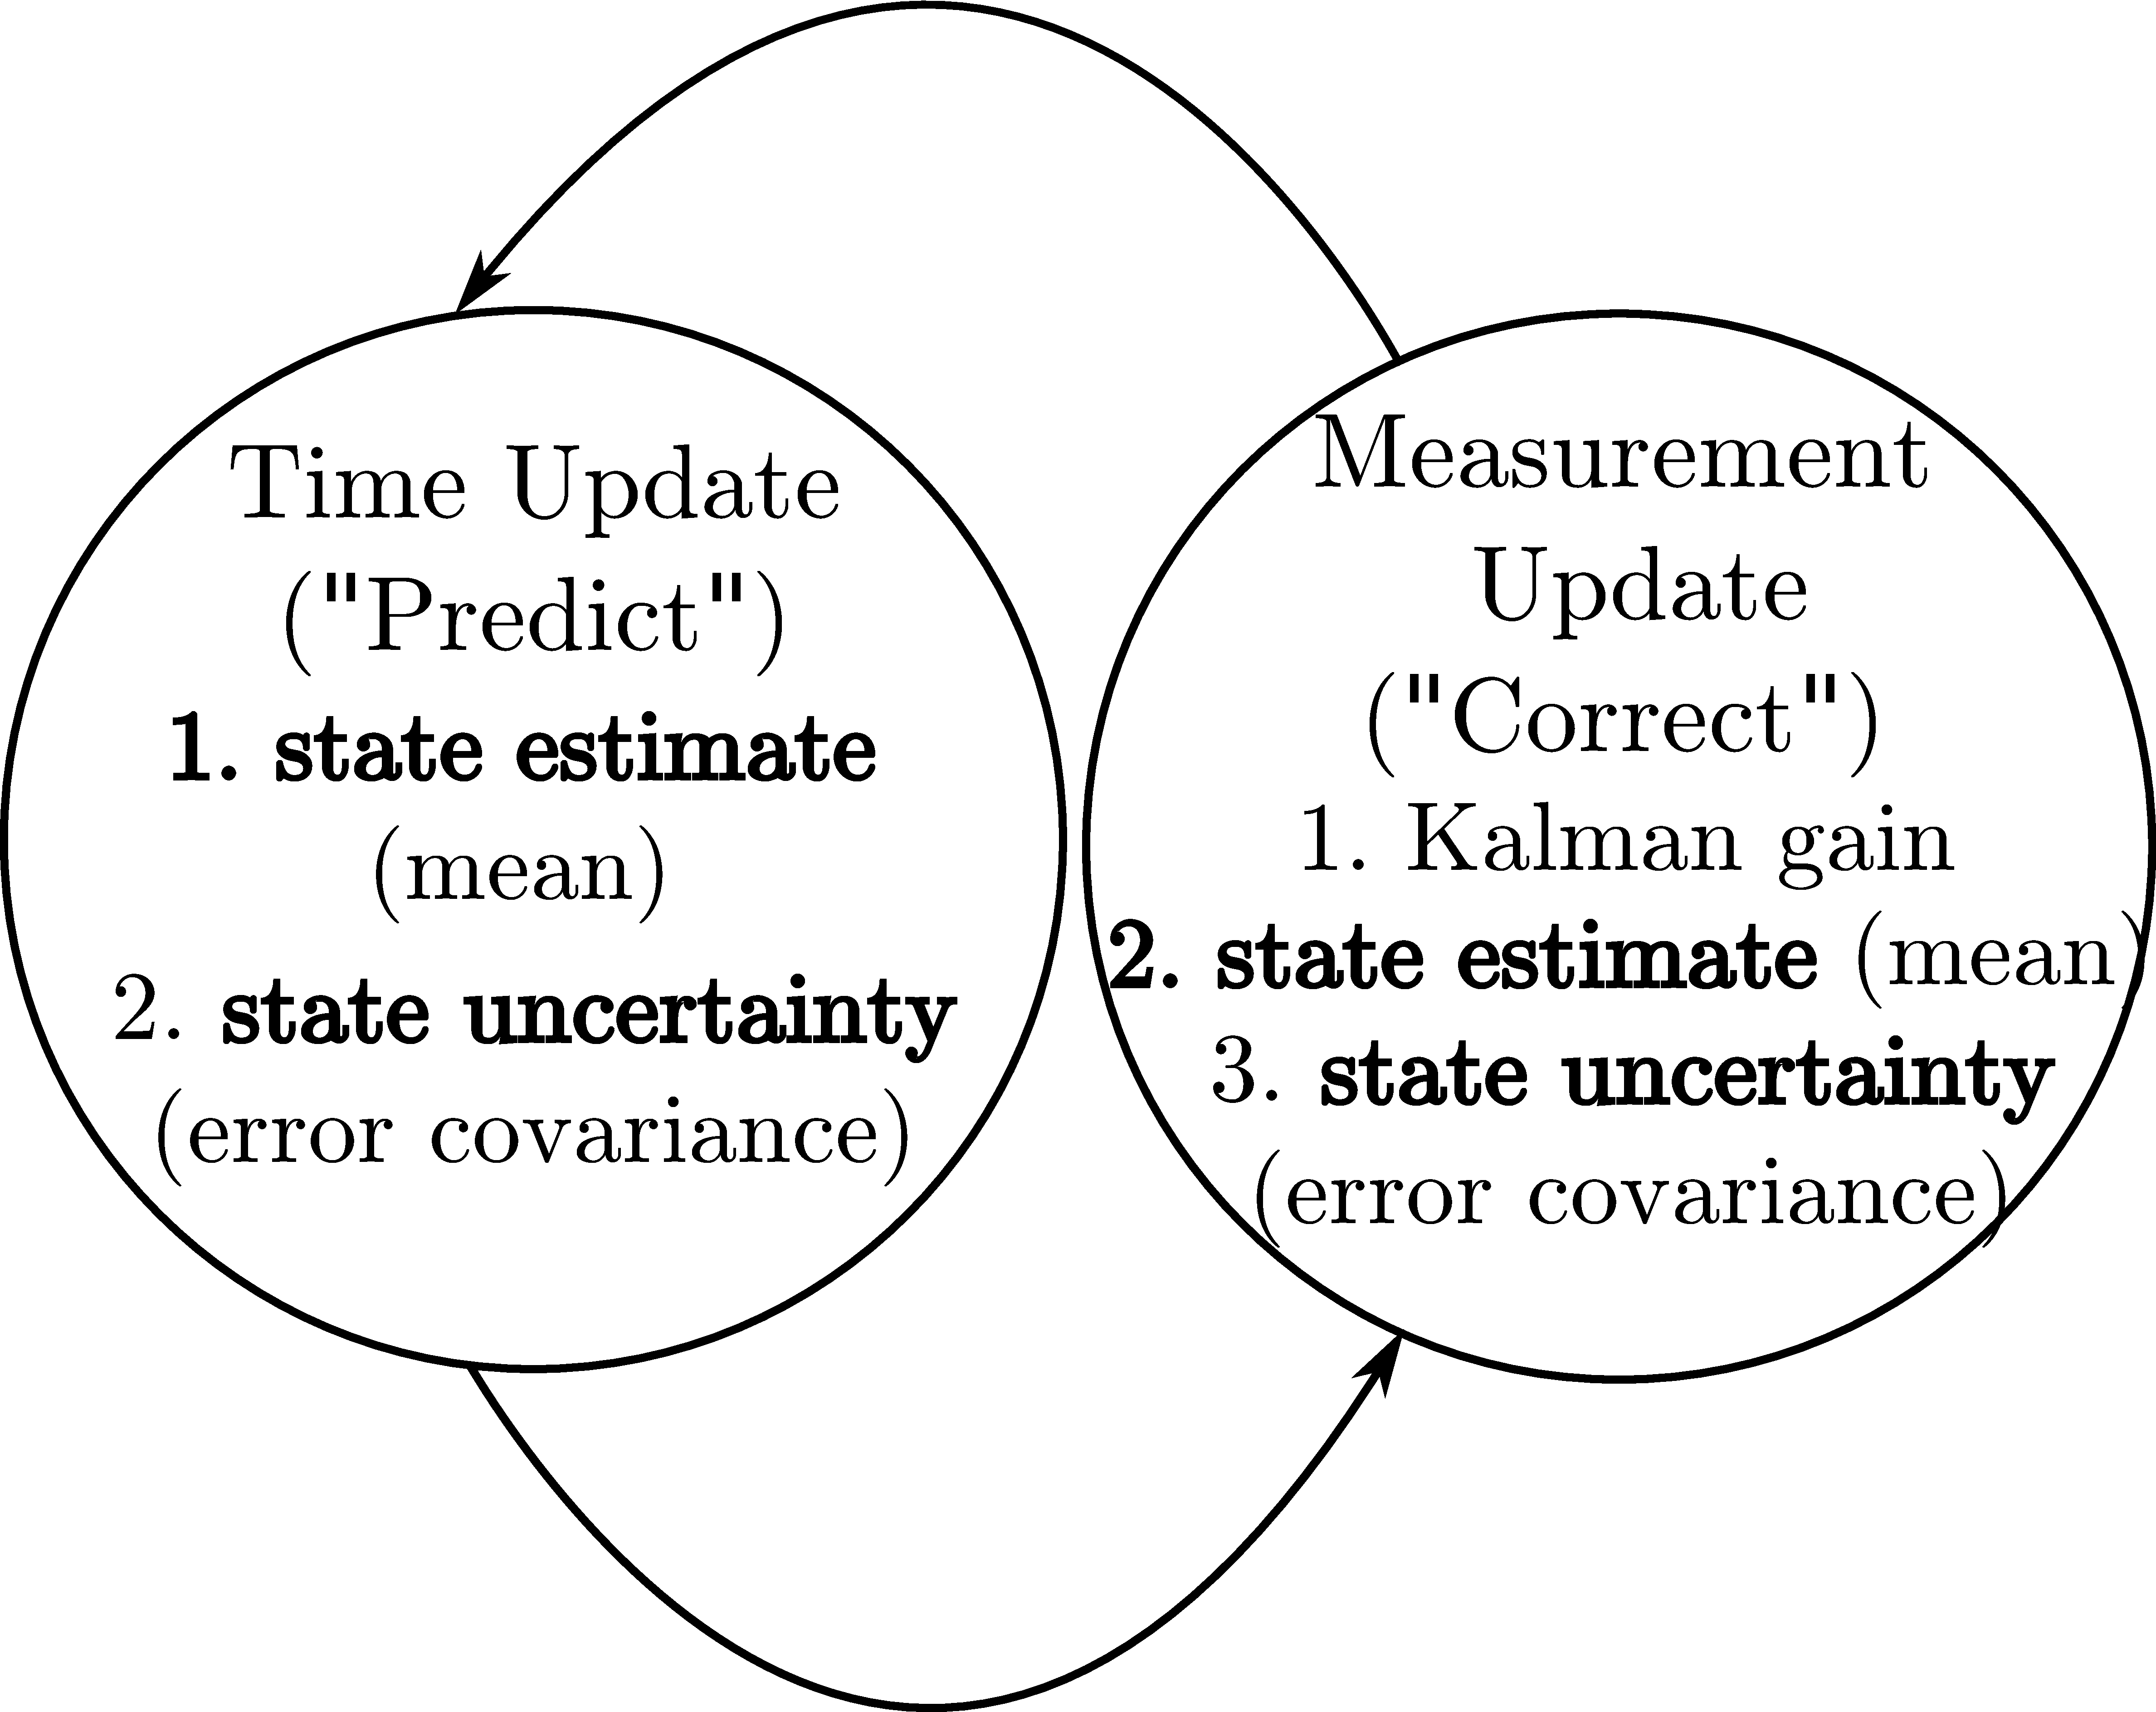
\includegraphics[width=0.85\linewidth]{fig/diagram-kalman.pdf}
	\end{block} 
\vspace{-25pt}	
	\begin{equation*} 
	\vect{X}(k) = f(\vect{X}(k-1), \vect{N}(k-1)) \; prediction
	\end{equation*}
\vspace{-25pt}	
	\begin{equation*}
	\vect{Z}(k) = h(\vect{X}(k), \vect{M}(k))  \; measurement%= \vect{H} \vect{X}(k \mid k-1)  + \vect{M}(k)
	\end{equation*}

\column{.45\textwidth}
\vspace{-5pt}
	\begin{itemize}
		\item \begin{footnotesize}``standard'' in nonlinear estimation, \textit{Bayesian} approach\end{footnotesize} %used in other applications - GPS, nav
		%\item \begin{footnotesize}\end{footnotesize}   % involving computing posterior PDF 
		\item \begin{footnotesize}$1^{st}$ order Taylor expansion of the nonlinear functions \end{footnotesize} 
		\item \begin{footnotesize}provides estimation uncertainties in form of error covariance matrices \end{footnotesize} 
		\item \begin{footnotesize}difficult tuning \end{footnotesize}
		\item \begin{footnotesize}reliable for systems that are almost linear on the time scale of the updates \end{footnotesize}
	\end{itemize}	
	%\begin{block}{Interesting alternative: Unscented Kalman Filter}
	%\end{block}
\end{columns}
\end{frame}

%%%%%%%%%%%%%%%%%%%%%%%%%%%%%%%%%%%%%%%%%%%%%%%%%%%%%%%%%%%%%%%%%%%%%%%%%%%%%%%

\begin{frame}\frametitle{Interesting alternative: Unscented Kalman Filter (UKF)}
The goal stays the same: to estimate the state $\vect{X}(k)$: mean ($\hat{X}$) and covariance ($P$). %Framework is similar: Nonlinear filter that does \textit{prediction \& correction}, uses Bayesian approach. \\
\vspace{-5pt}
\begin{columns}
	\column{.45\textwidth}
	\begin{block}{e.g. Mapping from Polar to Cartesian coordinates}
	\centering
	\begin{figure}
	\subfigure[{\scriptsize polar coord.}]{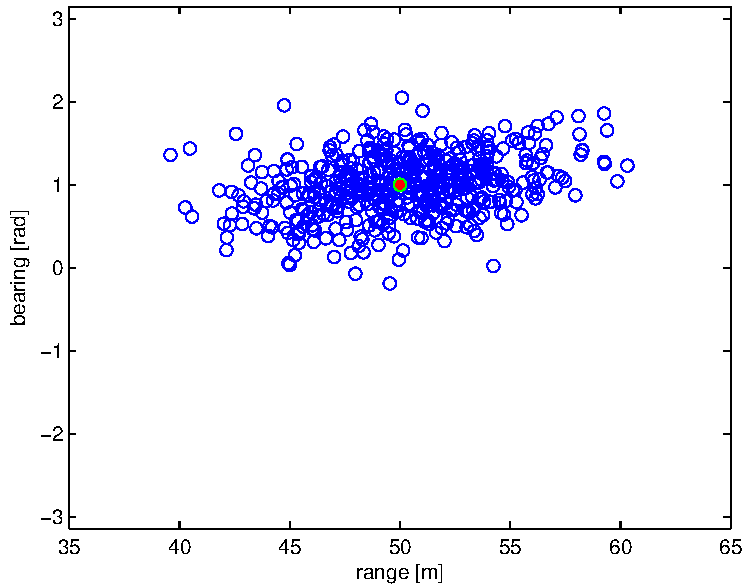
\includegraphics[width=0.45\linewidth]{fig/orig.pdf}}
	\subfigure[{\scriptsize $\hat{X}, P$ (EKF)}]{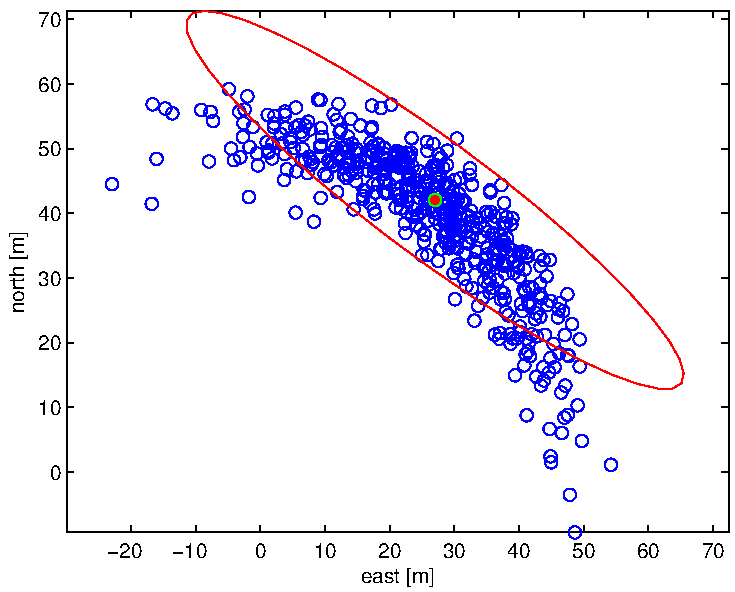
\includegraphics[width=0.45\linewidth]{fig/linear.pdf}} \\
	\subfigure[{\scriptsize UT sampled}]{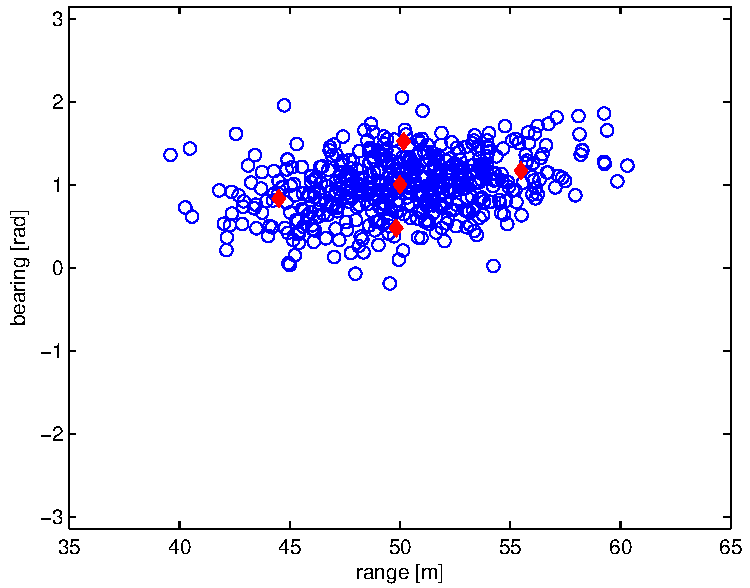
\includegraphics[width=0.45\linewidth]{fig/orig-samples.pdf}}
	\subfigure[{\scriptsize $\hat{X}, P$ (UKF)}]{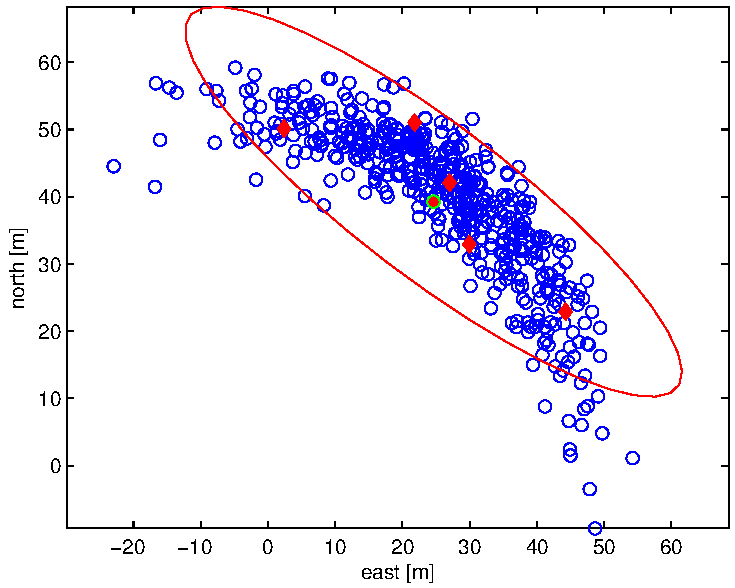
\includegraphics[width=0.45\linewidth]{fig/unscented.pdf}} \\
	\end{figure}
	\end{block} 

\column{.48\textwidth}
%\centering 
\vspace{-10pt}
\begin{columns}
\column{.38\textwidth}
\begin{block}{EKF}
{\scriptsize linearisation of the transform}
\end{block}
%\textbf{EKF} \\
%
\column{.58\textwidth}
\begin{block}{UKF}
{\scriptsize pdf is estimated using a collection of samples of a GRV propagated through the nonlinear transformation}
\end{block}
%\textbf{UKF} \\
%
\end{columns}
\vspace{5pt}
\textbf{Unscented Transform} (UT): selects the samples of a Gaussian and assigns a weight to each. 
	\begin{itemize}
		\item {\footnotesize guarantees $2^{nd}$ order Taylor expansion accuracy \cite{julier96}} 
		\item {\footnotesize no infamous Jacobians} 
		\item {\footnotesize same computational cost as EKF} 
	\end{itemize}	
\end{columns}
\end{frame}

%%%%%%%%%%%%%%%%%%%%%%%%%%%%%%%%%%%%%%%%%%%%%%%%%%%%%%%%%%%%%%%%%%%%%%%%%%%%%%%

\begin{frame}\frametitle{Sensor Fusion}%EKF implements sensor fusion. 
Sensor measurements are not available all the time - messages from sensors arrive at different moments and sensors could be unavailable due to different causes. 
\vspace{-5pt}
\begin{columns}
\column{.7\textwidth}
	\center{
    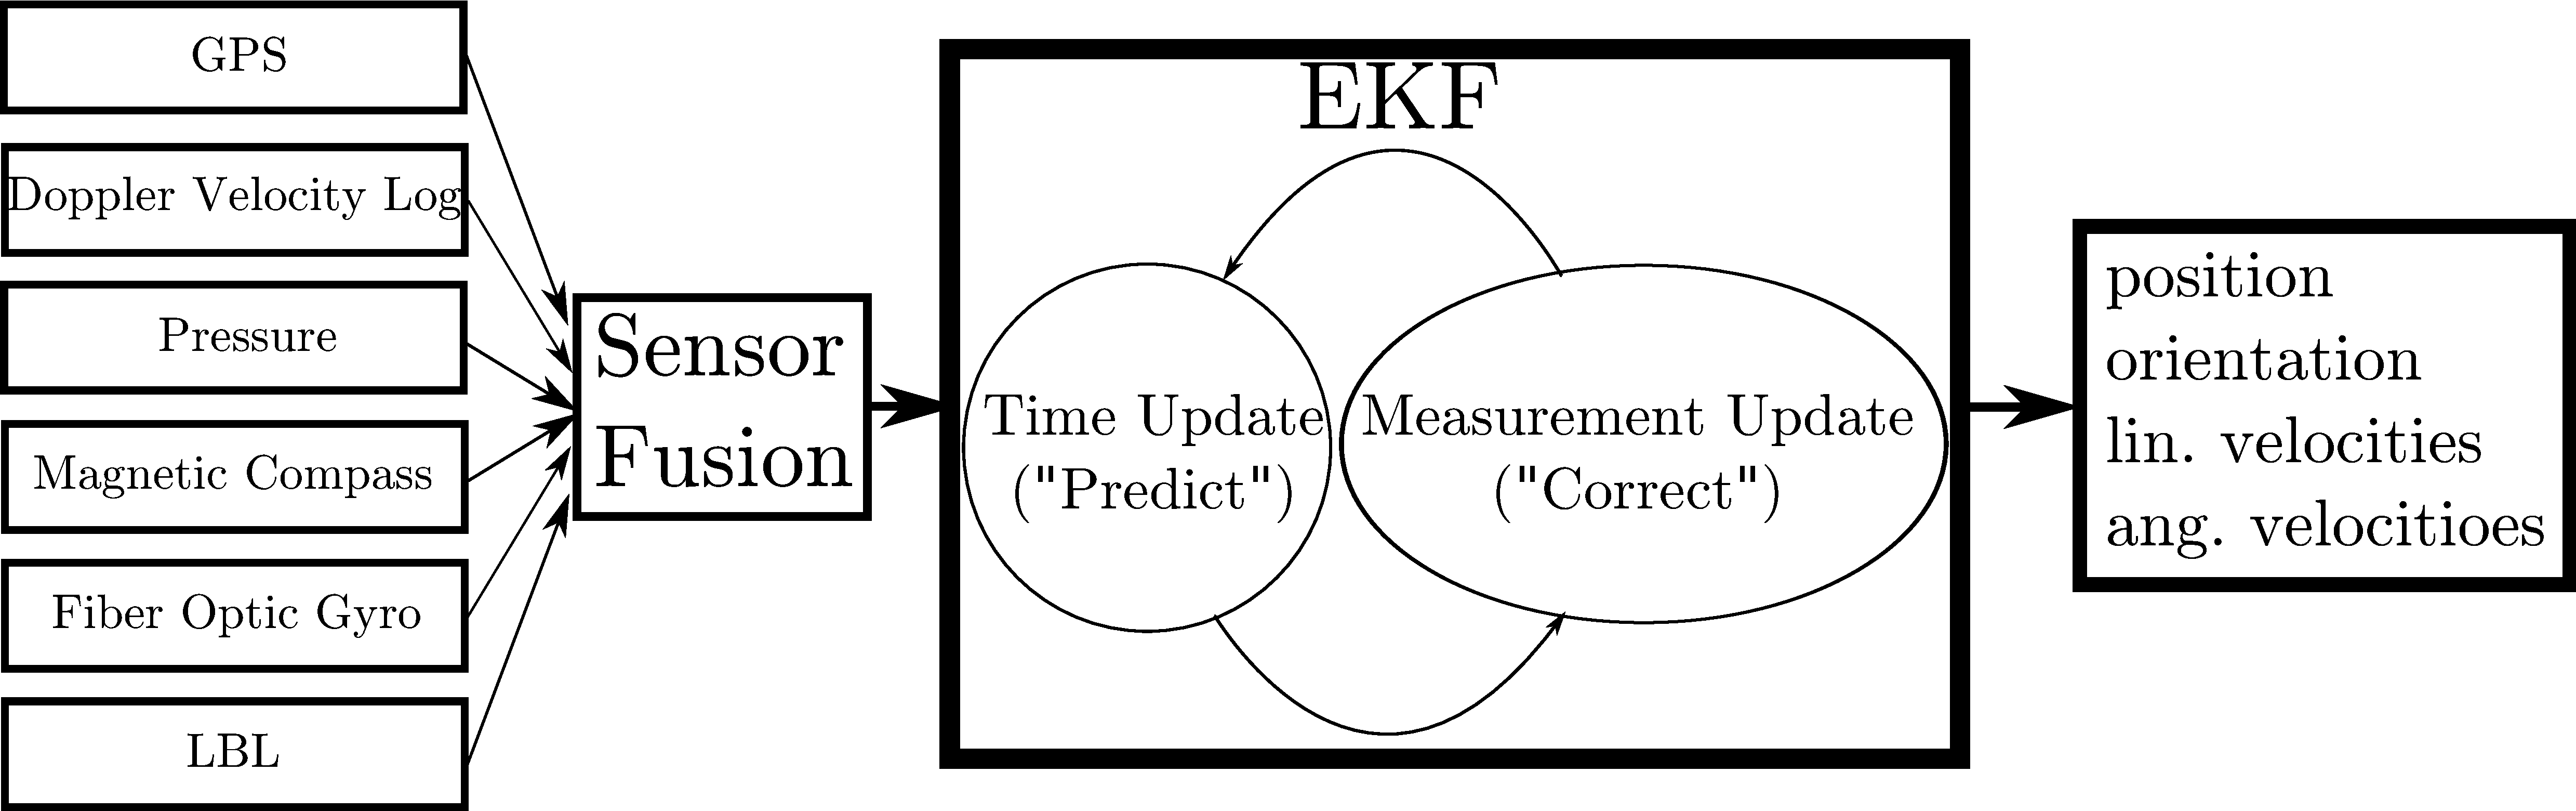
\includegraphics[width=0.98\linewidth]{fig/fusion-all.pdf}} \\
	\vspace{-5pt}
\hspace{3em} 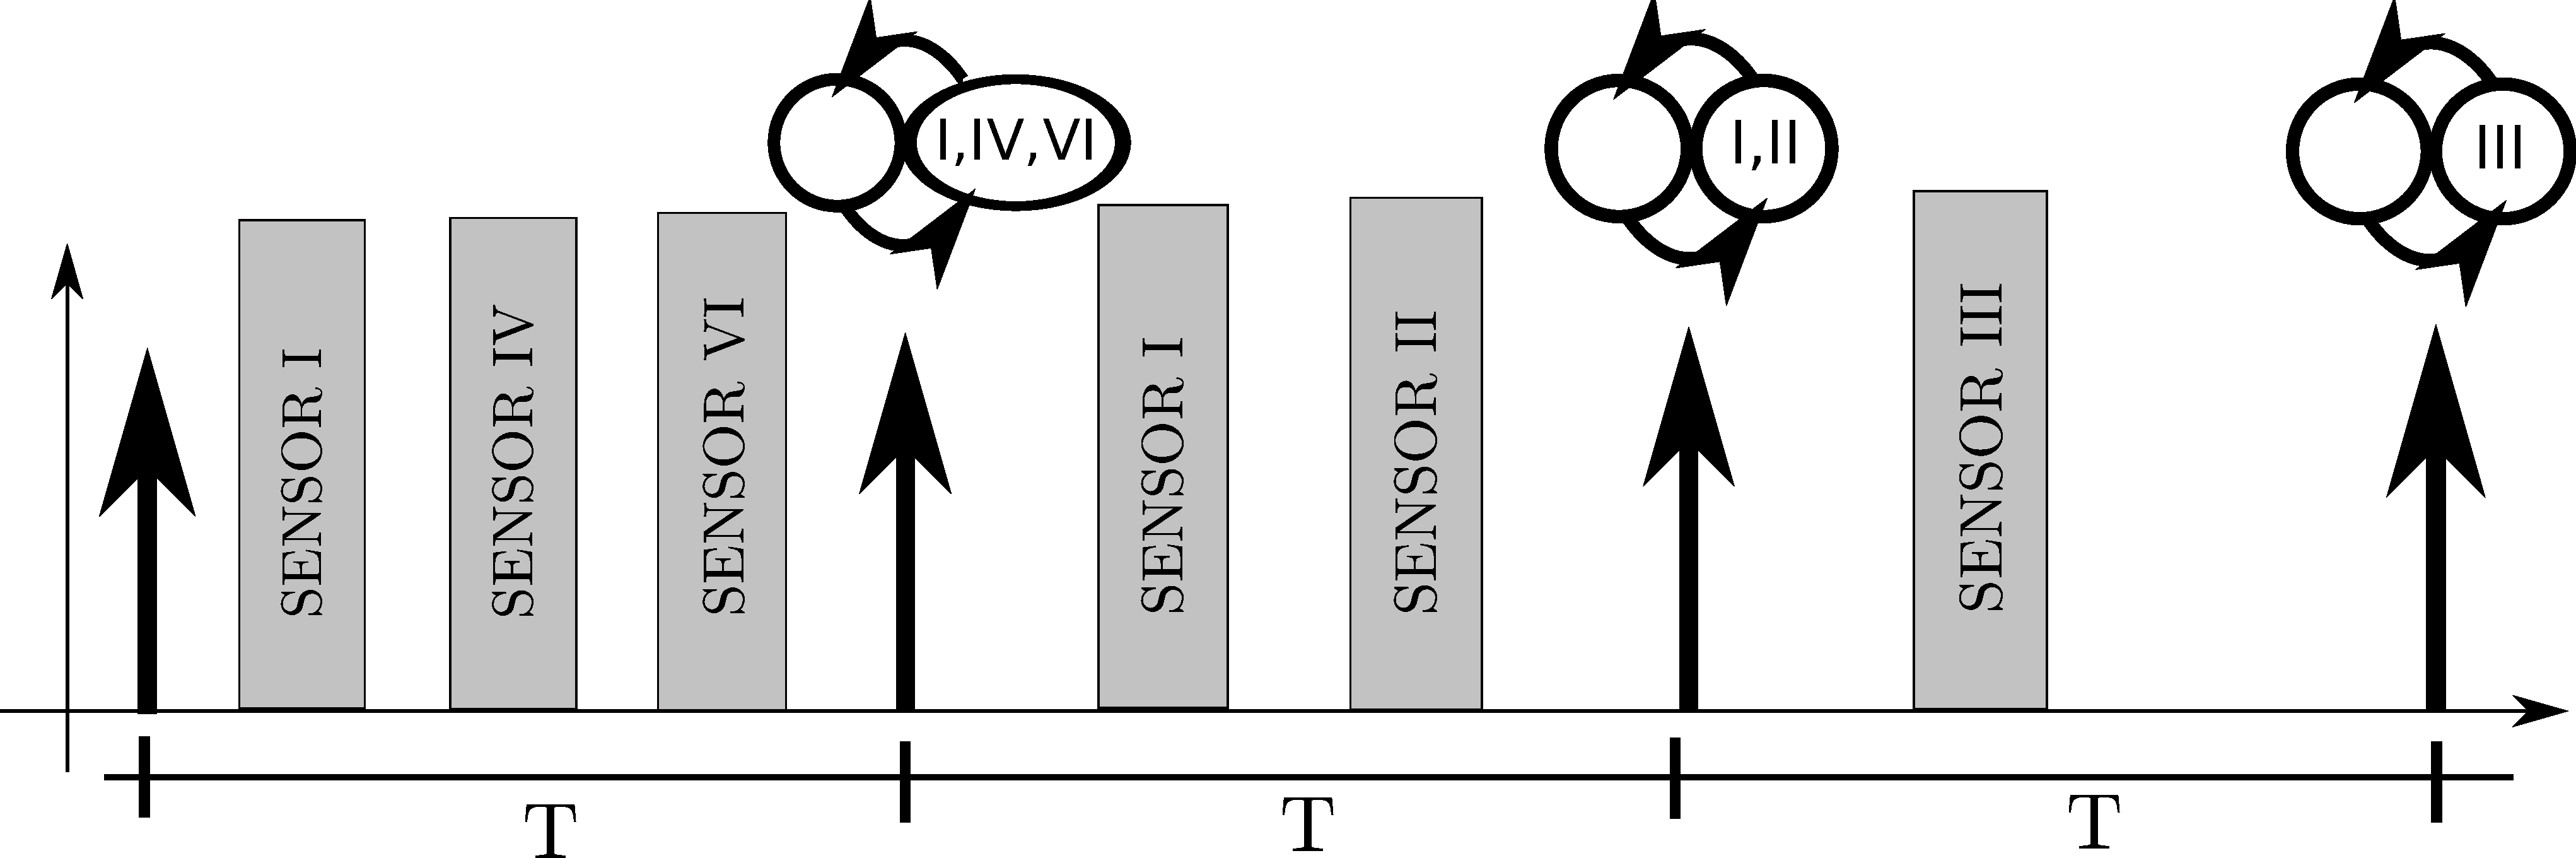
\includegraphics[width=0.43\linewidth]{fig/synch.pdf} 
\column{.28\textwidth}
	Gather the information in between the cycles and integrate it together in the measurement model (Eq. ~\ref{eq:fuse}).%, which varies depending on the measured values and sensors used for the measurement.
\end{columns}	
\begin{equation}
\label{eq:fuse}
\vect{Z}(k) = \left[ \begin{array}{c} \vect{Z}_{sen. I} \\ \vect{Z}_{sen. II}  \end{array} \right],
\vect{H}(k) = \left[ \begin{array}{c} \vect{H}_{sen. I} \\ \vect{H}_{sen. II}  \end{array} \right], 
\vect{R}(k) = \left[ \begin{array}{cc} \vect{R}_{sen. I} & 0 \\ 0 & \vect{R}_{sen. II} \end{array} \right]
\end{equation}
\vspace{-10pt}	
	\begin{equation*}
	\vect{Z}(k) = h(\vect{X}(k), \vect{M}(k)) = \vect{H} \vect{X}(k \mid k-1)  + \vect{M}(k)
	\end{equation*}
%parameters 
$\vect{R}_{sen. I}$ and $\vect{R}_{sen. II}$ are defining sensor measurement (un)certainty.
\end{frame}

%%%%%%%%%%%%%%%%%%%%%%%%%%%%%%%%%%%%%%%%%%%%%%%%%%%%%%%%%%%%%%%%%%%%%%%%%%%%%%%

\begin{frame}\frametitle{Why Kalman?}
\begin{columns}[t]
\column{.49\textwidth}
\textbf{I. Blending the measurements}\\ %\begin{block}{}
\vspace{-1em}
\begin{center}
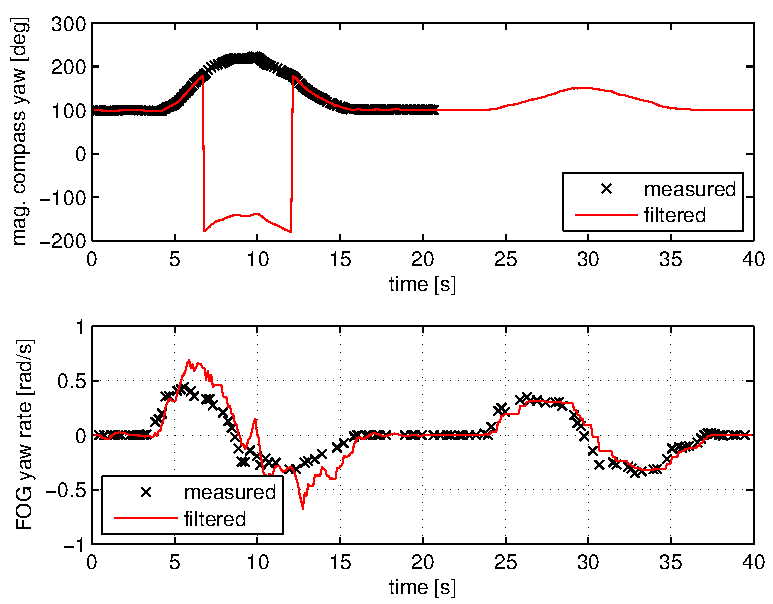
\includegraphics[width=0.8\linewidth]{fig/lostCompass.pdf}
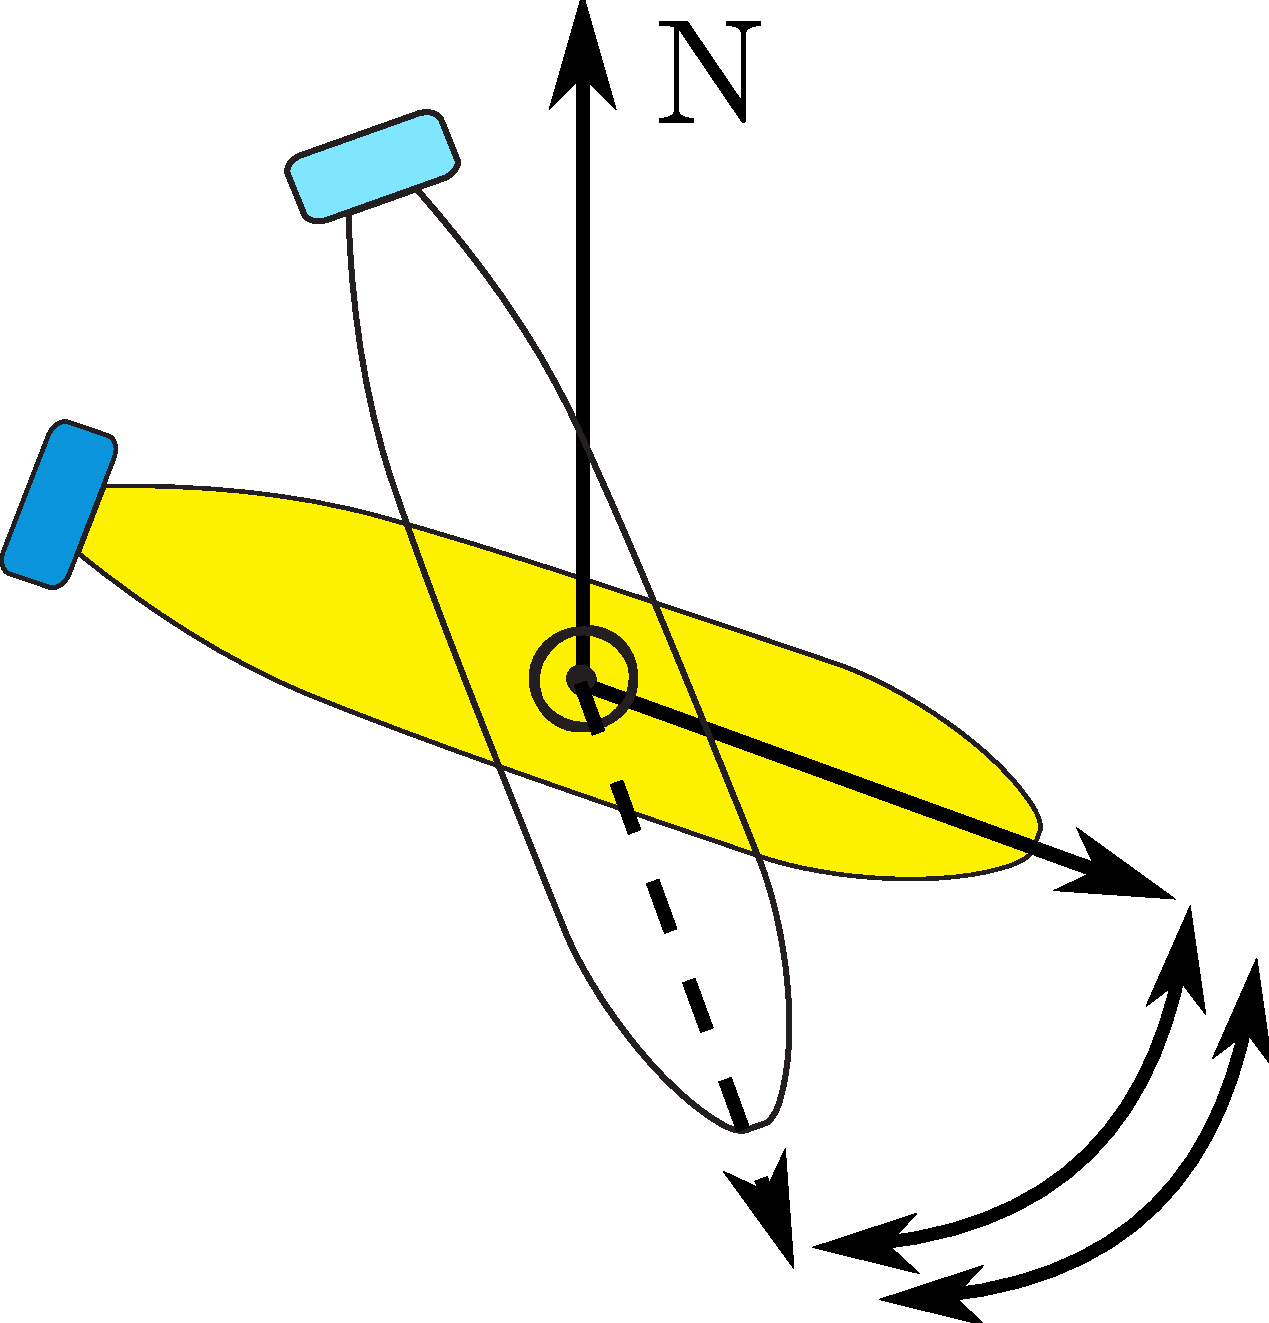
\includegraphics[width=0.19\linewidth]{fig/rotate.pdf} \\
\end{center}
\vspace{-1em}
yaw $(\psi)$ is inferred from compass \& FOG.\\
\textit{EKF benefit}: \pro if one of them stops working - the other one tries to compensate the failure

			\column{.49\textwidth}%$\Rightarrow$ 
			\textbf{II. Prediction \& Filtering} \\ %\begin{block}{}
			If the measurement temporarily fails, EKF keeps predicting. Noisy velocity information is filtered. \\%, with increased uncertainty. \\
			\centering
			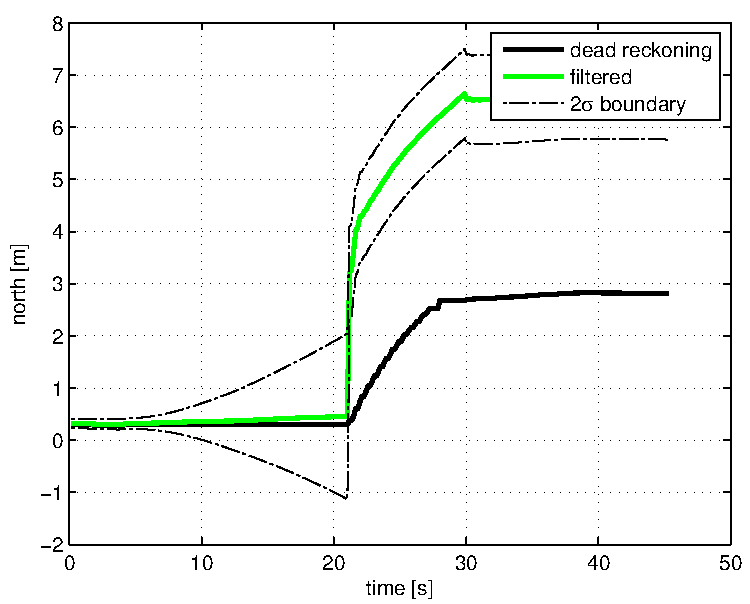
\includegraphics[width=0.49\linewidth]{fig/northLengthPool.pdf} 
			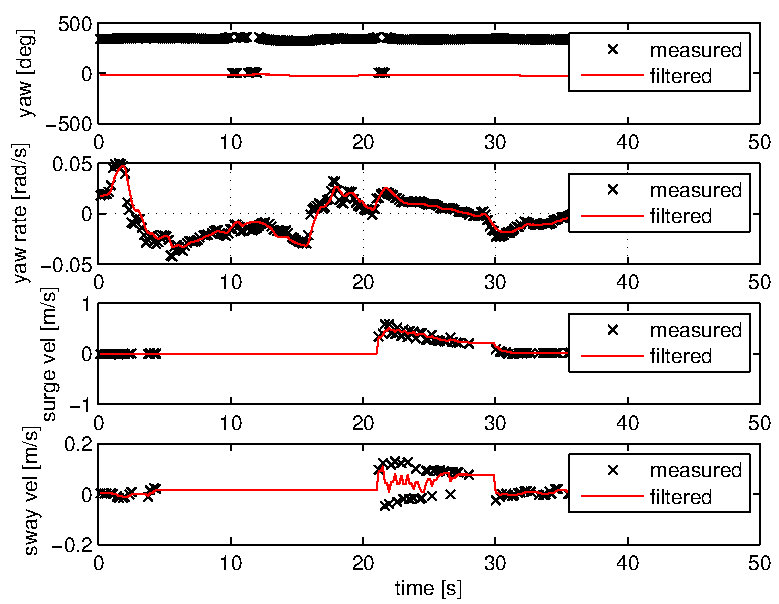
\includegraphics[width=0.49\linewidth]{fig/dynLengthPool.pdf}\\
			\textit{Outcome}: \pro less drift \\
			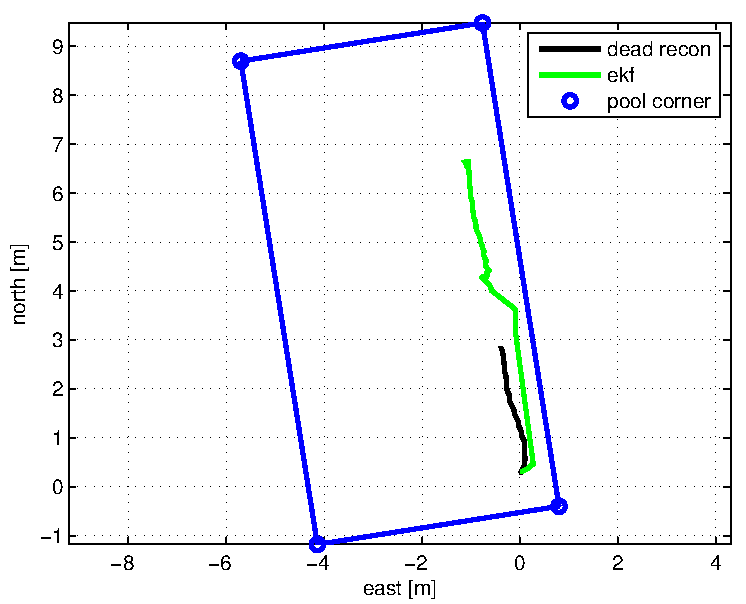
\includegraphics[width=0.5\linewidth]{fig/lengthPool.pdf}  \hspace{0.5em} 
			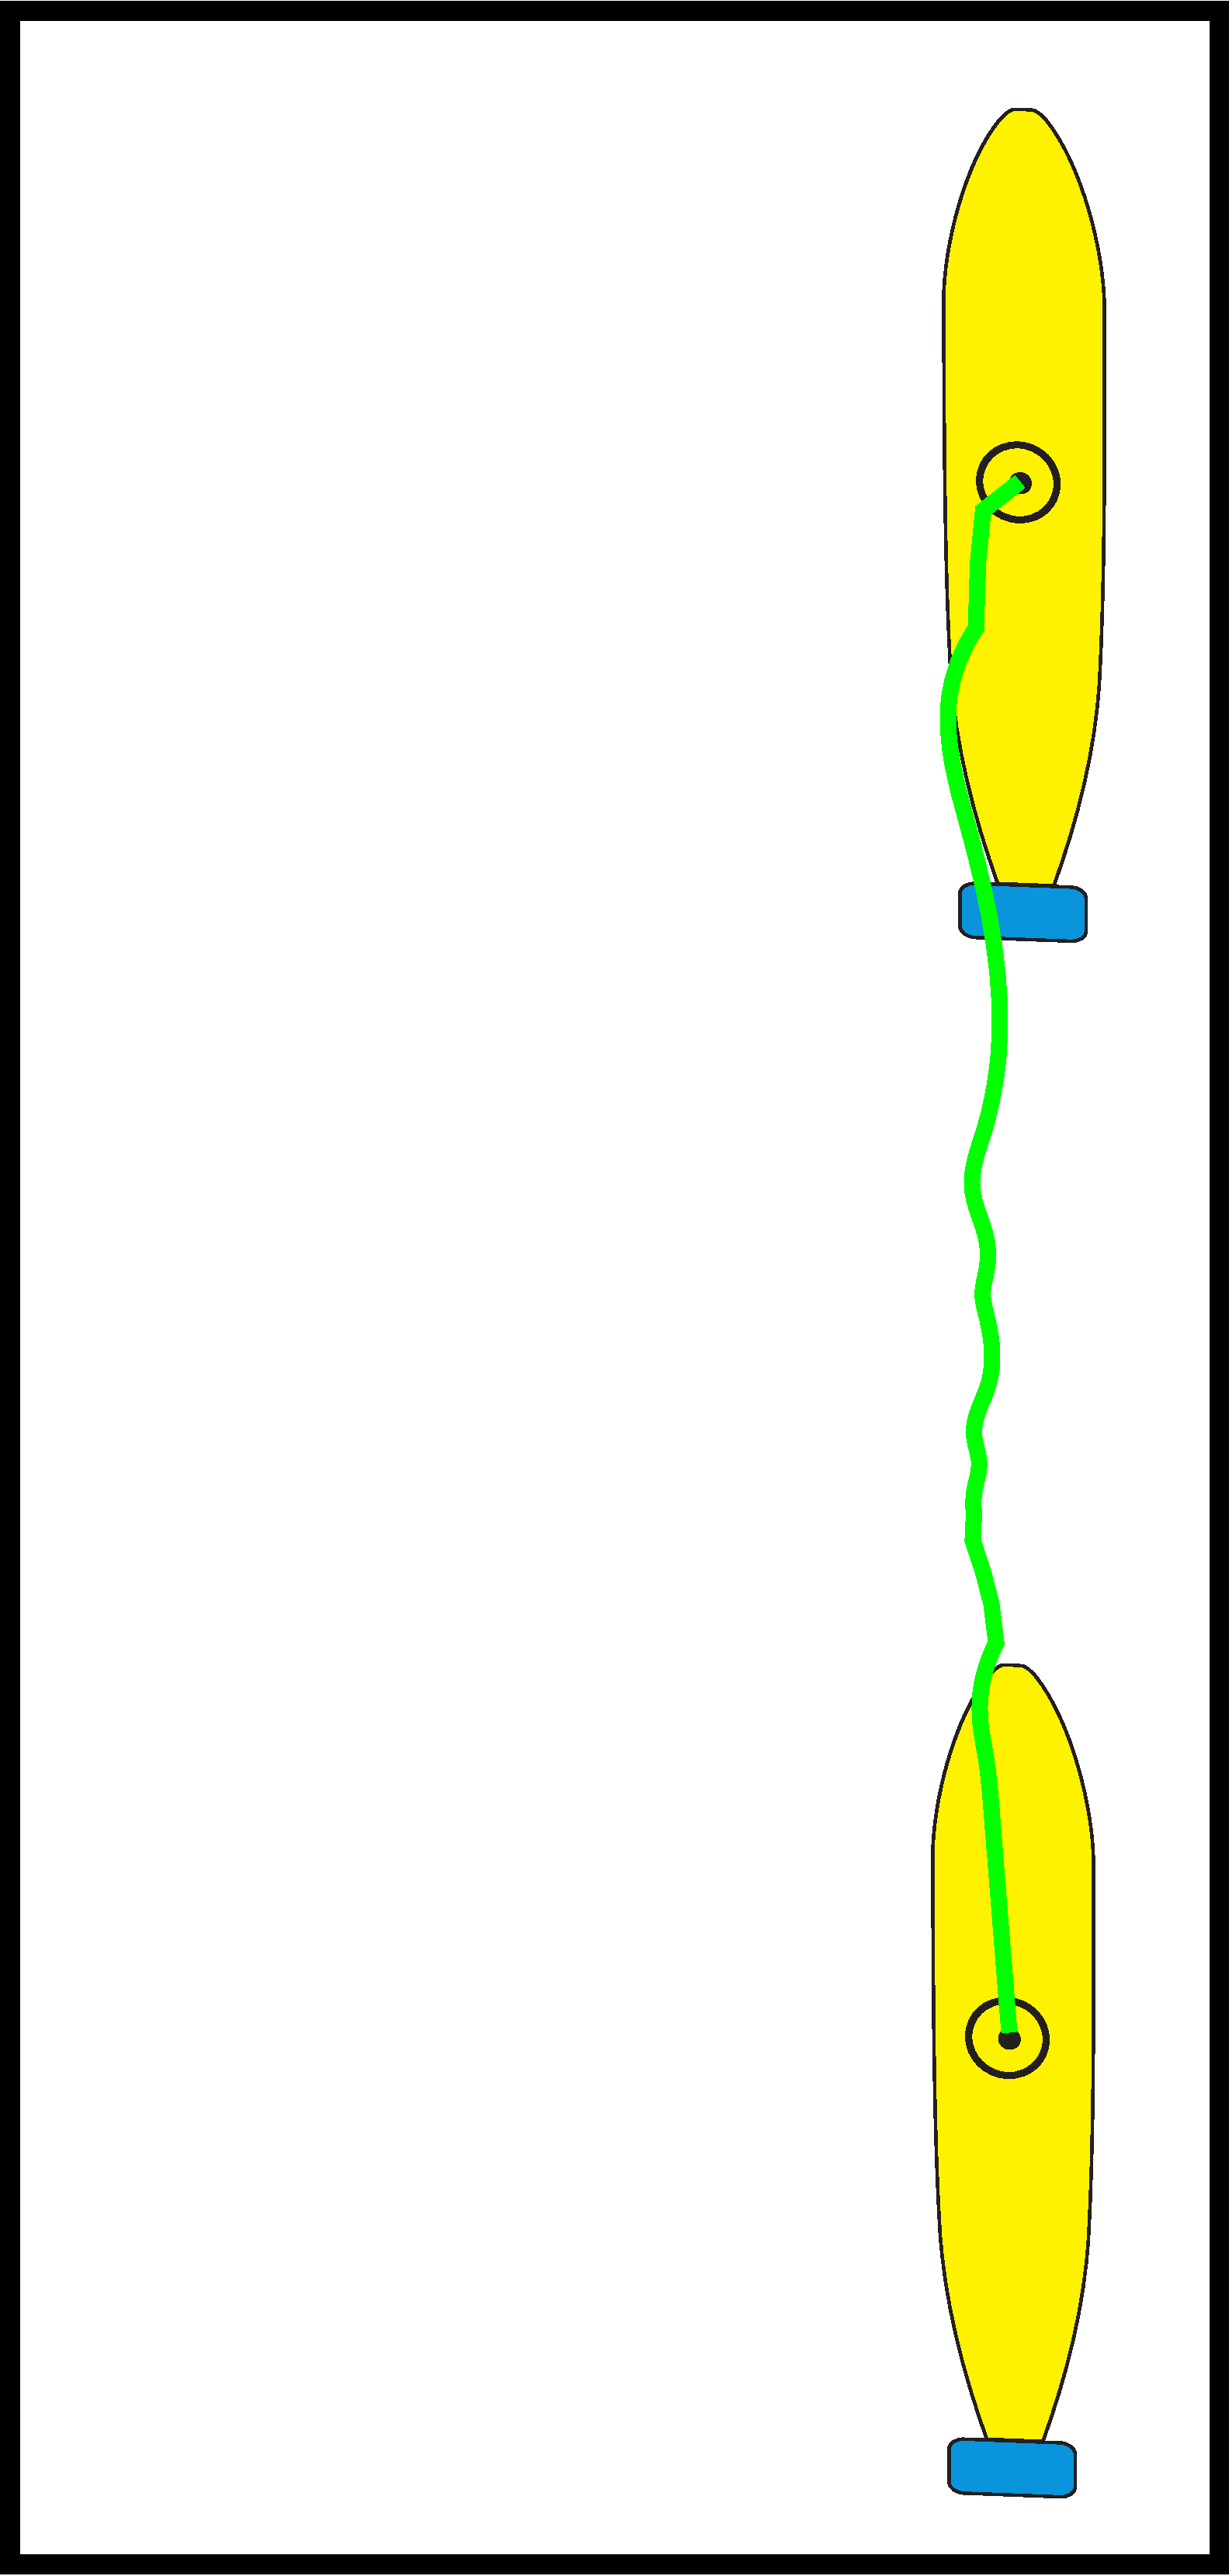
\includegraphics[width=0.15\linewidth]{fig/path.pdf} 
\end{columns}
\textbf{III. Parametric Estimation: }
setting the values of model and observation noise covariance matrices dozes the ``trust'' in model/measurements. 
\end{frame}

%%%%%%%%%%%%%%%%%%%%%%%%%%%%%%%%%%%%%%%%%%%%%%%%%%%%%%%%%%%%%%%%%%%%%%%%%%%%%%%

\begin{frame}\frametitle{Performing Localisation in Real Missions}
\begin{block}{Spiral surfacing trajectory}
\begin{columns}
\column{.7\textwidth}
Spiral trajectory and surfacing action was taken with Nessie starting from the depth of around 12 m (Fig. ~\ref{fig:spiral}). %Trajectory seems to be smoother and less prone to drift . %Standard deviation of north and east measurement noise can be set 
\column{.28\textwidth}
\centering
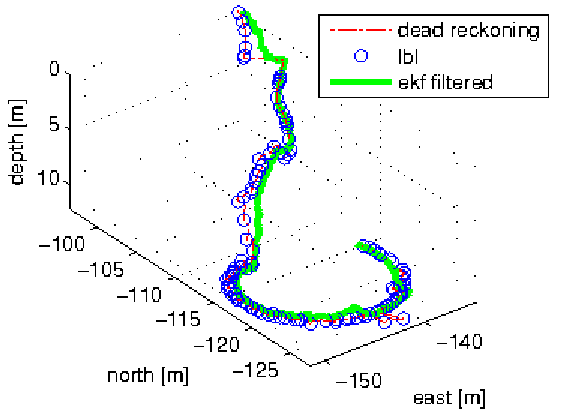
\includegraphics[width=0.7\linewidth]{fig/spiral3d.pdf}
\end{columns}
\end{block} 
\centering 
\begin{figure}
\vspace{-15pt}
\caption{Spiral trajectory localisation}
\vspace{-15pt}
\subfigure[{\scriptsize N/E localisation}]{\label{fig:ne2d}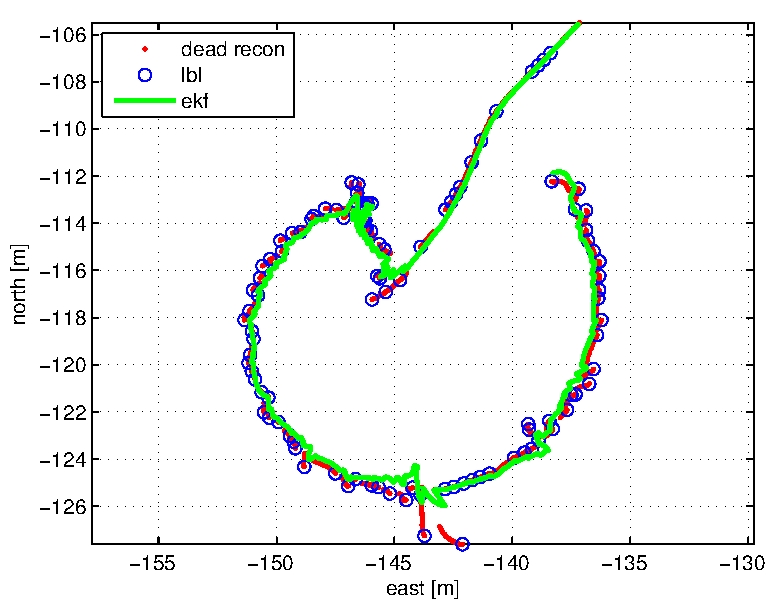
\includegraphics[width=0.45\linewidth]{fig/spiral2d.pdf}}
\subfigure[{\scriptsize depth filtering}]{\label{fig:depth}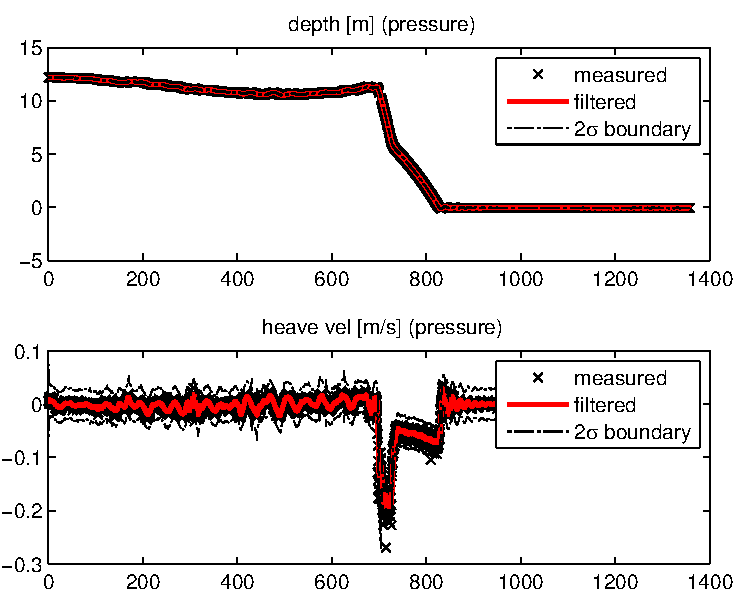
\includegraphics[width=0.45\linewidth]{fig/spiral-depth.pdf}} \\
\label{fig:spiral}
\end{figure}
%\begin{columns}[t]
%\column{.5\textwidth}
%\column{.2\textwidth}
\end{frame}

%%%%%%%%%%%%%%%%%%%%%%%%%%%%%%%%%%%%%%%%%%%%%%%%%%%%%%%%%%%%%%%%%%%%%%%%%%%%%%%


\begin{frame}\frametitle{AUV Localisation using EKF in Practise}
\vspace{-5pt}
\begin{block}{}
\center{\textbf{There is no is no exact ground truth for underwater robot localisation available}}
\end{block} 
\centering
Issues to Address in AUV Localisation%\end{center}
\begin{columns}[t]
\column{.36\textwidth}
{\centering \textbf{Heading Measurement}} \\
{\centering \hspace{6pt} 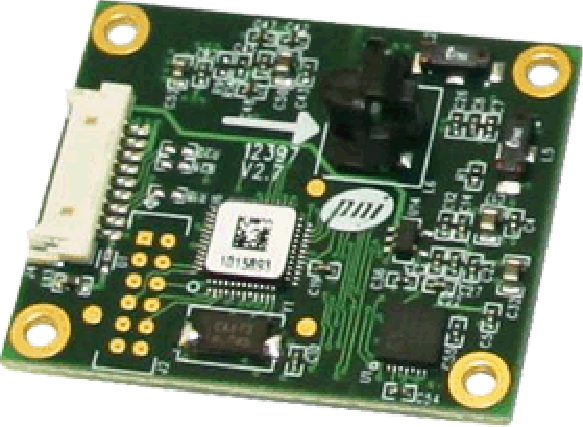
\includegraphics[width=0.25\linewidth]{fig/tcm.pdf} \hspace{15pt} vs.
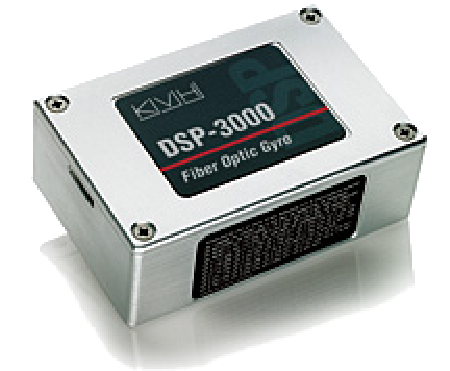
\includegraphics[width=0.25\linewidth]{fig/kvh.pdf}} \\
	\begin{columns}[t]
	\column{.55\linewidth}
	{\centering	
	Compass {\footnotesize(\textit{yaw})} } \\
	\contra \begin{footnotesize}prone to noise\end{footnotesize} \\
	\contra \begin{footnotesize}calibration\end{footnotesize} \\
	\pro    \begin{footnotesize}absolute\end{footnotesize}  \\ %  meas.	
		
	\column{.44\linewidth}
	{\centering	
	Gyro \\ {\footnotesize(\textit{yaw rate})} \\
	\pro    \begin{footnotesize}accurate\end{footnotesize}	\\
	\contra \begin{footnotesize}relative\end{footnotesize}  \\
	} %  meas.
	\end{columns}
\vspace{10pt}
Apart from being ``fused'', measurements of \textit{yaw rate} and \textit{yaw} can be taken with adjustable confidence. 	
\column{.3\textwidth}
{\centering \textbf{Nonlinearity}} \\
UKF \cite{julier96} is an interesting alternative in handling nonlinearities. 
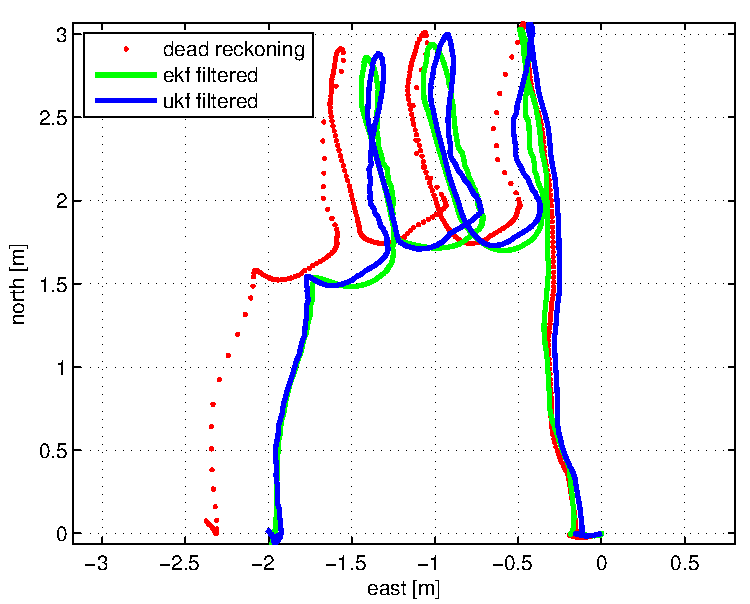
\includegraphics[width=0.85\linewidth]{fig/UKFpipeTrack.pdf} \\
\pro {\footnotesize model emulation} \\
\pro {\footnotesize computational cost}
\column{.31\textwidth} % on filtering those outliers. (absolute position)
{\centering \textbf{LBL imprecision}} \\ %LBL measurements exhibit quite diverse range of values. 
Position updates can deviate from the trajectory, resulting in outliers. EKF was compared with median filter.  \\  
{\centering
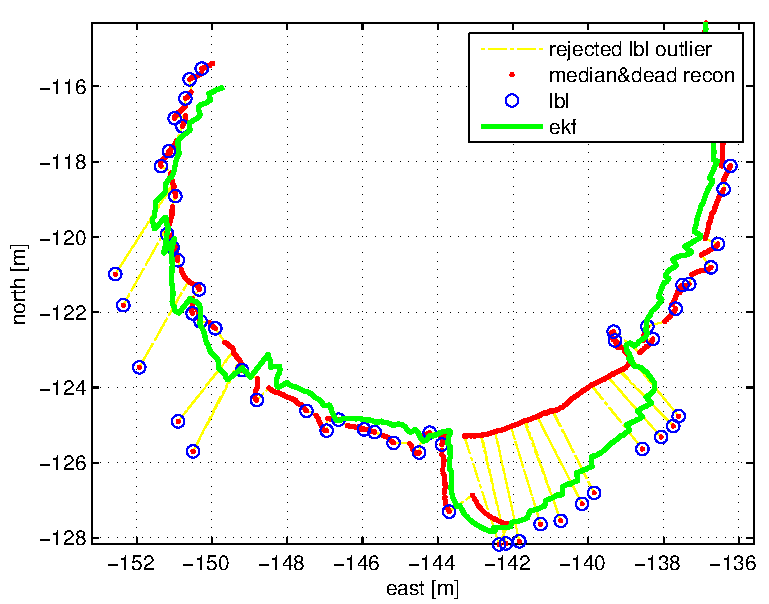
\includegraphics[width=0.8\linewidth]{fig/spiral-median-ekf.pdf} \\
\pro robust
} %outlier filtering 
\end{columns}
\end{frame}

%%%%%%%%%%%%%%%%%%%%%%%%%%%%%%%%%%%%%%%%%%%%%%%%%%%%%%%%%%%%%%%%%%%%%%%%%%%%%%%

\begin{frame}\frametitle{Performing Localisation in Real Missions}
\begin{block}{Rectangular trajectory in low depth}
\begin{columns}
\column{.78\textwidth}
Fairly noisy GPS signal (antenna is on the surface) was used as position correction. Parameters $\sigma_{north},\sigma_{east}$ of north and east measurement noise can be set (~\ref{fig:ne10}, ~\ref{fig:ne05}). Reasonably chosen values significantly correct the result obtained with pure dead reckoning. %Giving extremely high confidence with such amount of noise does not seem to be the best choice, however,
\column{.2\textwidth}
\centering
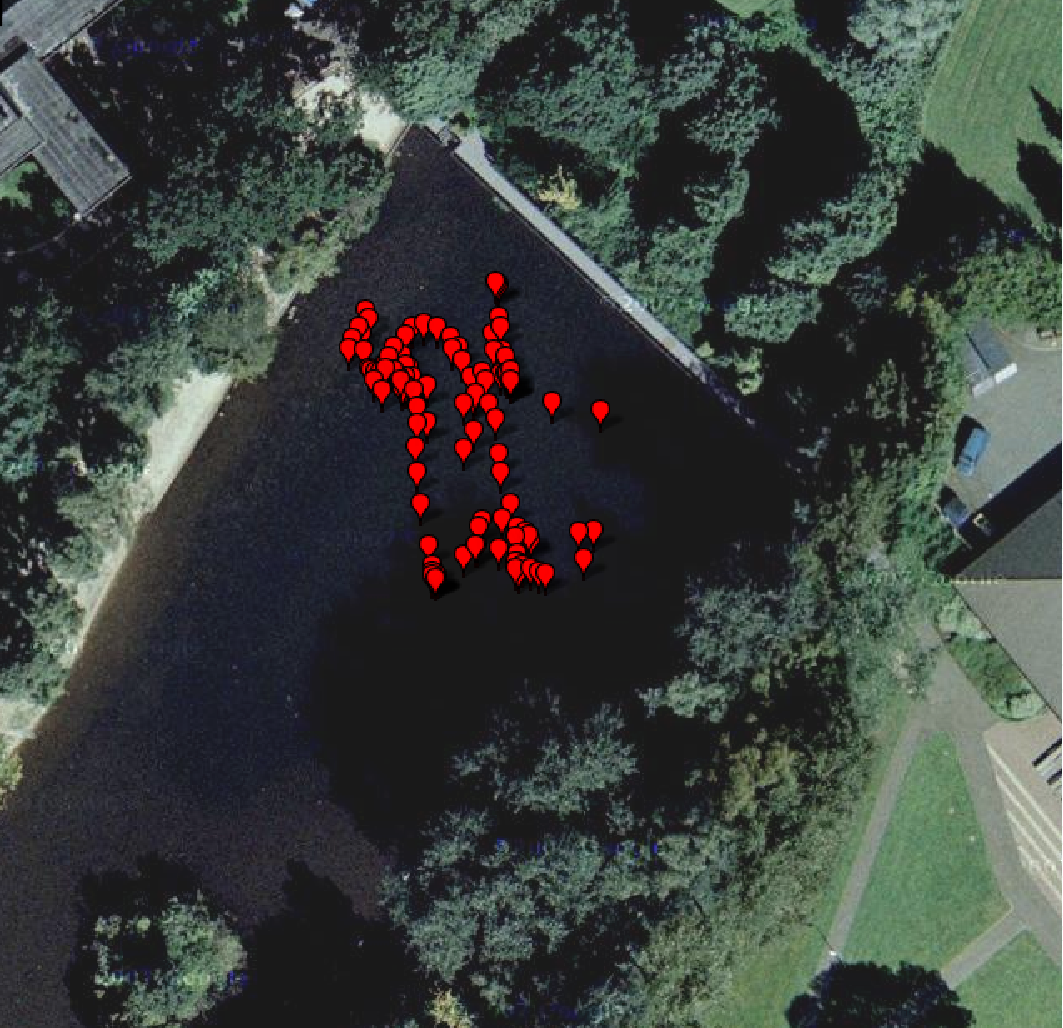
\includegraphics[width=0.95\linewidth]{fig/square-trajectory.pdf}
\end{columns}
\end{block}
\vspace{-10pt}
\centering 
\begin{figure}%(confidence in position measurement)  _{north}=\sigma_{east}  a_{north}=\sigma_{east}
\subfigure[{\scriptsize N/E localisation $\sigma= 1.0 m $}]{\label{fig:ne10} 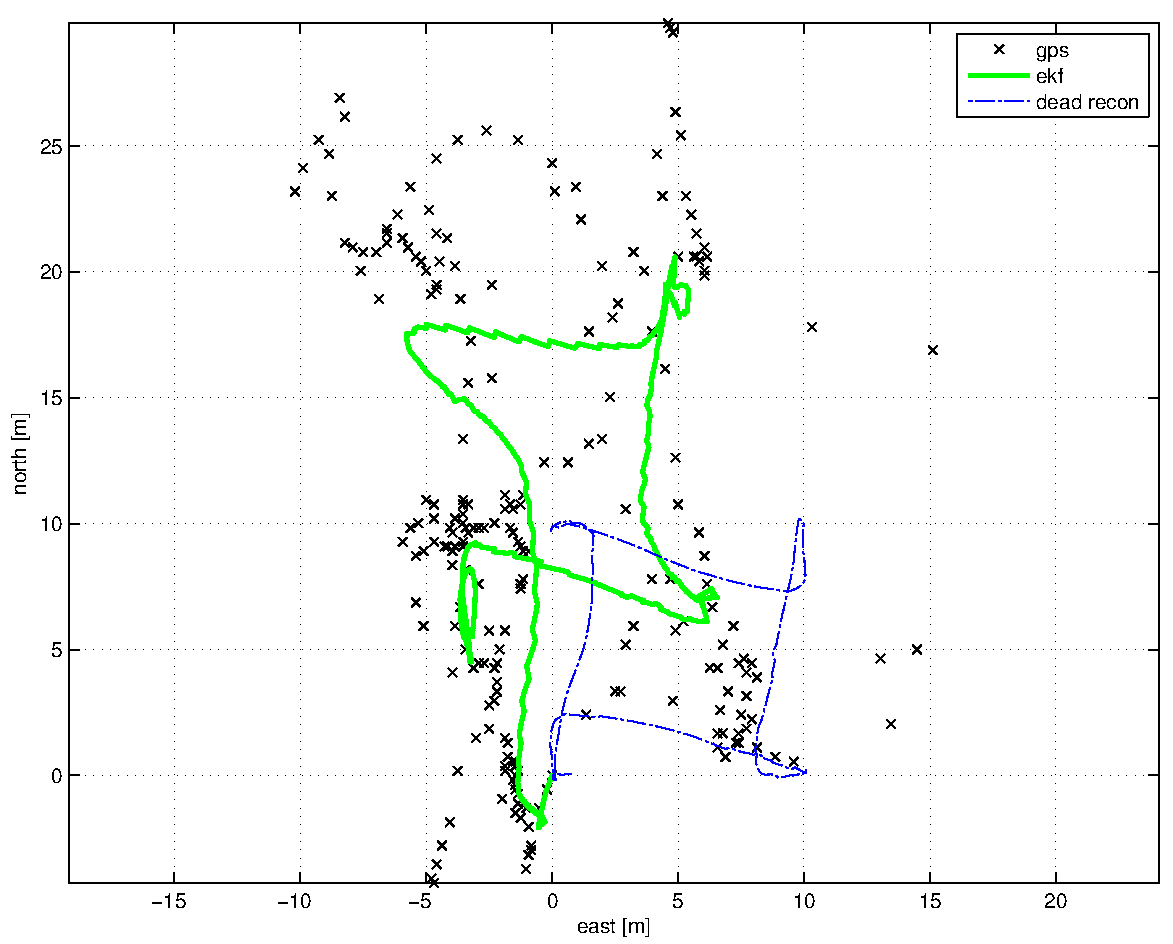
\includegraphics[width=0.32\linewidth]{fig/square10.pdf}} 
\subfigure[{\scriptsize N/E localisation $\sigma= 0.5 m $}]{\label{fig:ne05} 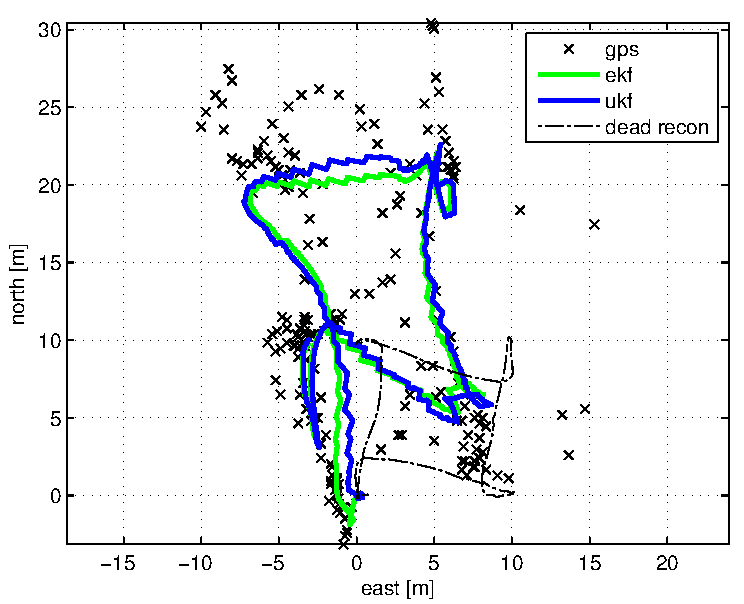
\includegraphics[width=0.32\linewidth]{fig/square05.pdf} }
\subfigure[{\scriptsize Velocities \& heading}]{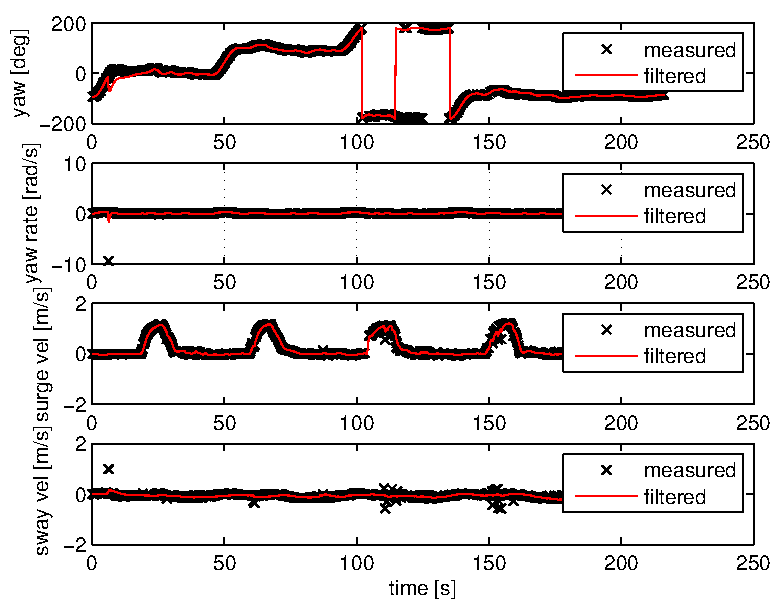
\includegraphics[width=0.3\linewidth]{fig/dynamics.pdf}}
\vspace{-10pt}
\caption{Rectangular trajectory localisation}
\vspace{-10pt}
\end{figure}
%From a noisy collection of position observations at the beginning, application of EKF with sensor fusion enabled having generally better performance in navigation.
\end{frame}

%%%%%%%%%%%%%%%%%%%%%%%%%%%%%%%%%%%%%%%%%%%%%%%%%%%%%%%%%%%%%%%%%%%%%%%%%%%%%%%

\begin{frame}\frametitle{Conclusions}
Presented work reports the design of an navigation module for a real AUV based on Extended Kalman Filter (EKF) .
\begin{itemize}
\item EKF proves to be useful navigation tool with satisfactory navigation performance and several convenient features: \\
{\scriptsize 
\hspace{0.5cm} capable of successfully combining together different sensory information (\textit{sensor fusion}) \\
\hspace{0.5cm} estimate that tends to be optimal with respect to set expectations \\
\hspace{0.5cm} recovering from the missing measurements \\
\hspace{0.5cm} filtering corrupted position information: outliers or signal noise \\
}
%EKF is a great tool since it tries to satisfy the set uncertainty boundaries and fuse all the available information trying to make the most out of it combined together in one mathematical system. %- ``filtration with semantics''
%\\
\item 5DOF \textit{constant velocity} mathematical model for state prediction was introduced 
%\\ One of the issues that were addressed was the s
\item Suitable management of heading measurement was addressed and the role of EKF in correcting deficiencies
%\\
%\item Sensor fusion was explored as mean of improving the estimation
%\\
\item Nonlinearity issues have been investigated with the usage of Unscented Kalman Filter (UKF)
\end{itemize} 
\end{frame}

%%%%%%%%%%%%%%%%%%%%%%%%%%%%%%%%%%%%%%%%%%%%%%%%%%%%%%%%%%%%%%%%%%%%%%%%%%%%%%%

\begin{frame}\frametitle{Future Work}
\begin{itemize}
\item More trials, particularly ones where the vehicle trajectory has been fixed to known landmarks so that the results of localisation could be thoroughly evaluated with trustful ground truth
%
% \\
%{\scriptsize 
%\hspace{0.5cm} capable of successfully combining together different sensory information (\textit{sensor fusion}) \\
%\hspace{0.5cm} estimate that tends to be optimal with respect to set expectations \\
%\hspace{0.5cm} recovering from the missing measurements \\
%\hspace{0.5cm} filtering corrupted position information, outliers, or signal noise \\
%}
%EKF is a great tool since it tries to satisfy the set uncertainty boundaries and fuse all the available information trying to make the most out of it combined together in one mathematical system. %- ``filtration with semantics''
%\\
\item Navigation of the tilted vehicle movements in order to make an evaluation of the influence of the 5th d.o.f

%\\ One of the issues that were addressed was the s
\item EKF could be improved so that it works with control inputs
%\\
%\item Sensor fusion was explored as mean of improving the estimation
%\\
\item Filtering of the noisy absolute position gives space for improvement. Solution for rejecting outliers could rely on some version of \textit{back-filtering} - filtering based on history of received observations.% since the measured position tends to be quite uncertain and prone to different sorts of noise. 


\end{itemize} 
\end{frame}

%%%%%%%%%%%%%%%%%%%%%%%%%%%%%%%%%%%%%%%%%%%%%%%%%%%%%%%%%%%%%%%%%%%%%%%%%%%%%%%
%\begin{frame}
%\frametitle{Kalman fusion strategy}
%Describe the algorithm used.
%\end{frame}
%%%%%
%\begin{frame}
%\frametitle{Localisation algorithm}
%Describe the algorithm used and the ones that were tested.
%\end{frame}
%%%%%
%\begin{frame}
%\frametitle{Graphical results}
%2d plots of some missions.
%Experimental results in real environment presented.
%\end{frame}
%%%%%%%%%%%%%%%%%%%%%%%%%%%%%%%%%%%%%%%%%%%%%%%%%%%%%%%%%%%%%%%%%%%%%%%%%%%%%%%

%\chapter{Results} \label{chap:results}
Main purpose of the thesis is the implementation of a navigation system that uses measurements from different sensors, fuses the sensory data together in order to make presumably better quality estimate of the position and the orientation of the underwater robot. Existing data from the real missions were used to carry out the initial trials. It is useful to mention that there is no exact ground truth for underwater robot localization available. GPS signal, if available, could serve as an absolute position reference: either directly or in form of LBL. Experimental results have been obtained for different missions. Good news, however, is that the absolute depth measurement is quite accurate and frequent, making AUV localisation a 2D task.  

\section{Real navigation scenario} \label{sec:real-scenario}
Authentic data taken from previously recorded Nessie mission were used to simulate the algorithm ``offline'' as the part of the stage intended for testing and correcting. Besides, being able to repeat the same measurement scenario enables more insight in filtering process and benefits of fusing together the sensor data. \textit{.bag} files (\url{http://www.ros.org/wiki/}) containing recorded real-time messages with sensor measurements, were used as source. Furthermore, it allows designing the code in its original C++ form that will require little modification once deployed on the vehicle in form of ROS package since \textit{.bag} files emulate authentic messages and timestamps. One of the deficiencies of the evaluation of localisation results is the fact that there is no exact ground truth to compare the result with. Dead reckoning localisation substituted with occasional LBL position updates was compared with the localisation obtained after filtering (Figures ~\ref{fig:auv-sim-straight2}, ~\ref{fig:auv-sim-straight1}) for the recorded straight line trajectory mission. 

\T{Selecting a heading measurement with good performance}
For a high-end underwater vehicle such as Nessie, supplied with FOG-based INS, DVL and LBL, main source of navigation error is influenced by transformation of vehicle-referenced velocities to world-referenced velocities \cite{bahr08}, particularly due to yaw (heading) measurement errors. Yaw can be measured using several devices, each having different accuracy and performance. Simulation with data from previous missions was carried out to see which device gives the best performance for a given underwater vehicle. 

Heading calculated by integrating FOG's yaw rate - tends to be accurate and fast, less prone to noise. Nevertheless, it is calculated each time by appending yaw rate value integrated in time on the previous yaw value (relative measurement). Therefore, it is sensible on initial absolute heading measurement. In case initial yaw is imprecise, a constant bias exists in yaw measurement (Figure ~\ref{fig:auv-sim-straight1}). Constant bias causes sudden steps in position estimate obtained using EKF. This is expected scenario since the sensor responsible for measuring initial heading is magnetic compass, device sensitive to disturbances coming from environment (Figure ~\ref{fig:magnetic-disturb}). In real experiments biggest obstacle was proper calibration of magnetic compass. In practice, tests have showed many failures in compass heading measurement, possibly due to calibration and magnetic declination. There is yet space to do more testing with better compass tuning. To overcome the problem of accurate yaw measurement, EKF used in experiments will either ignore the yaw measurement (it is possible since sensor fusion successfully compensates missing heading information with yaw rate obtained from FOG) or use it with high variance assigned to yaw measurement. 
%Finally, initial heading is given with magnetic compass.

\T{Loch Earn dataset - straight line movement}: Example of basic EKF localisation using inertial measurements aided with LBL acoustic positioning system was tested on straight line movement of approximately 80 m length, recorded at the lake Loch Earn. For simulation purposes, sensor measurements are stored in a \textit{.bag} file, that can be replayed, producing real-time messages of sensor measurements as they originally occurred. At this point, it is important to revise which sensors were used, their main features and, finally, filtering parameters. 

Standard sensor configuration comprising of pressure sensor, magnetic compass, FOG and DVL is used in the mission. Absolute position correction was carried out using LBL system. Important fact is that the heading was measured with magnetic compass only at the beginning. Later on, it kept being calculated by integrating yaw rate obtained from FOG. Alternative solution for the heading measurement would be the usage of compass for direct acquiring of yaw, but such option exposed calibration difficulties. Result of EKF localisation algorithm was shown in north-east map (Figure ~\ref{fig:sim-straight2}, ~\ref{fig:sim-straight1}). Different parameter values for EKF were tested. Table ~\ref{tab:ekf-params} revises all filter parameters used for filter tuning, together with their role. Essentially, setting high standard deviation for a Gaussian of a certain parameter can be interpreted as having more uncertainty in value that it represents - whether it is a measurement uncertainty or uncertainty of the predicted value (model uncertainty). Therefore, we can choose to be confident in certain sensor measurement and/or certain model prediction, and observe the simulation outcome of such setting. Setting the parameters properly improves the performance of the filter.  
\addtocounter{footnote}{1}
\footnotetext[\value{footnote}]{as it appears in algorithm equations}  
\begin{table*}
\centering
	\caption{EKF navigation parameters.}
	\label{tab:ekf-params}
\begin{tabular}{llll}
\toprule
Parameter      &     Signature $^{\decimal{footnote}}$     &     Units     &    Description  \\
\midrule
                         & \multicolumn{3}{c}{standard deviation of the ... } \\ 
\multirow{1}{*}{SDNorth} & \multirow{1}{*}{$\sigma_{n}$} & \multirow{1}{*}{$m$} & \multirow{1}{*}{north observation} \\
\multirow{1}{*}{SDEast}  & \multirow{1}{*}{$\sigma_{e}$} & \multirow{1}{*}{$m$} & \multirow{1}{*}{east observation} \\
\multirow{1}{*}{SDDepth} & \multirow{1}{*}{$\sigma_{d}$} & \multirow{1}{*}{$m$} & \multirow{1}{*}{depth observation} \\
\multirow{1}{*}{SDAltitude} & \multirow{1}{*}{$\sigma_{a}$} & \multirow{1}{*}{$m$} & \multirow{1}{*}{altitude observation} \\
\multirow{1}{*}{SDu} & \multirow{1}{*}{$\sigma_{u}$} & \multirow{1}{*}{$\frac{m}{s}$} & \multirow{1}{*}{surge velocity observation} \\
\multirow{1}{*}{SDv} & \multirow{1}{*}{$\sigma_{v}$} & \multirow{1}{*}{$\frac{m}{s}$} & \multirow{1}{*}{sway velocity observation} \\
\multirow{1}{*}{SDw} & \multirow{1}{*}{$\sigma_{w}$} & \multirow{1}{*}{$\frac{m}{s}$} & \multirow{1}{*}{heave velocity observation} \\
\multirow{1}{*}{SDyaw} & \multirow{1}{*}{$\sigma_{\psi}$} & \multirow{1}{*}{$rad$} & \multirow{1}{*}{heading observation} \\
\multirow{1}{*}{SDpitch} & \multirow{1}{*}{$\sigma_{\varphi}$} & \multirow{1}{*}{$rad$} & \multirow{1}{*}{pitch observation} \\
\multirow{1}{*}{SDyawRate} & \multirow{1}{*}{$\sigma_{\dot{\psi}}$} & \multirow{1}{*}{$\frac{rad}{s}$} & \multirow{1}{*}{heading rate observation} \\
\multirow{1}{*}{SDpitchRate} & \multirow{1}{*}{$\sigma_{\dot{\varphi}}$} & \multirow{1}{*}{$\frac{rad}{s}$} & \multirow{1}{*}{pitch rate observation} \\
\midrule
                         & \multicolumn{3}{c}{standard deviation of the ... process noise} \\
\multirow{1}{*}{SDuModel} & \multirow{1}{*}{$\sigma_{\dot{u}}$}  & \multirow{1}{*}{$\frac{m}{s^{2}}$} & \multirow{1}{*}{surge acceleration} \\
\multirow{1}{*}{SDvModel} & \multirow{1}{*}{$\sigma_{\dot{v}}$}  & \multirow{1}{*}{$\frac{m}{s^{2}}$} & \multirow{1}{*}{sway acceleration} \\
\multirow{1}{*}{SDwModel} & \multirow{1}{*}{$\sigma_{\dot{w}}$}  & \multirow{1}{*}{$\frac{m}{s^{2}}$} & \multirow{1}{*}{heave acceleration} \\
\multirow{1}{*}{SDyawRateModel} & \multirow{1}{*}{$\sigma_{\dot{v}}$}  & \multirow{1}{*}{$\frac{rad}{s^{2}}$} & \multirow{1}{*}{yaw acceleration} \\
\multirow{1}{*}{SDpitchRateModel} & \multirow{1}{*}{$\sigma_{\dot{w}}$}  & \multirow{1}{*}{$\frac{rad}{s^{2}}$} & \multirow{1}{*}{pitch acceleration} \\
\bottomrule
\end{tabular} 
\end{table*}
Straight line movement with authentic sensor measurements recorded in Loch Earn was a basis for initial tests of the EKF localisation algorithm. Red line shows the dead reckoning navigation, which is directly updated with absolute position update (LBL). Dead reckoning uses values periodically ($\approx$5$Hz$) obtained from DVL and FOG (linear velocities: $u$ and $v$ and heading $\psi$, respectfully), and substitutes them into equations similar to ones used for north and east prediction within prediction model: 
$$ north = north + (uT+\dot{u}\frac{T^{2}}{2})\cos(\psi) - (vT+\dot{v}\frac{T^{2}}{2})\sin(\psi) $$
$$ east  = east  + (uT+\dot{u}\frac{T^{2}}{2})\sin(\psi) + (vT+\dot{v}\frac{T^{2}}{2})\cos(\psi) $$
% SDnorth/east = 5 $cm$, 
% SDnorth/east = 5 $cm$, 
\begin{figure}%[htb]
  \centering
    \subfigure[N/E localisation. Yaw was calculated by integrating yaw rate periodically measured using FOG.] {\label{fig:sim-straight2}
	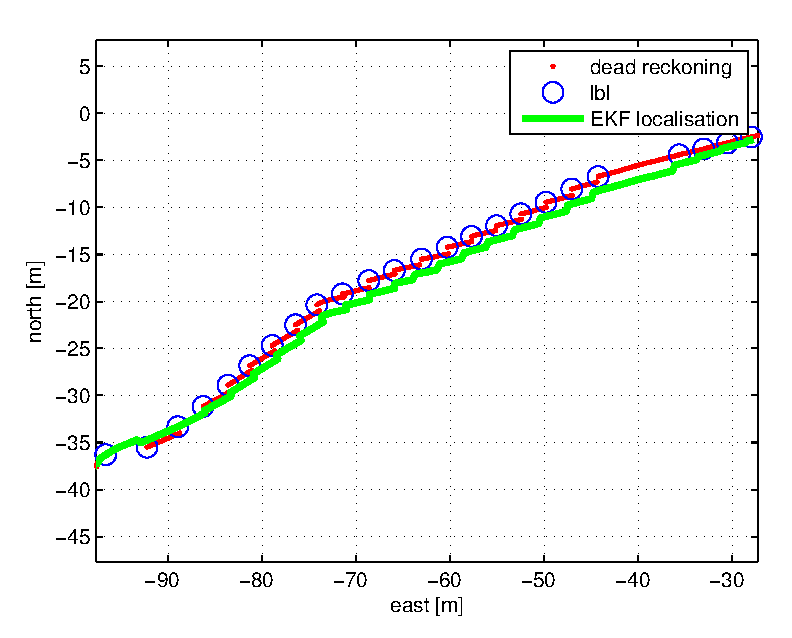
\includegraphics[width=0.48\linewidth]{simulations/fig/sim-straight2.eps}}
    \subfigure[Heading estimation. Biased yaw measurement not being corrected due to high confidence in yaw measurement.] {\label{fig:yaw-straight2}
    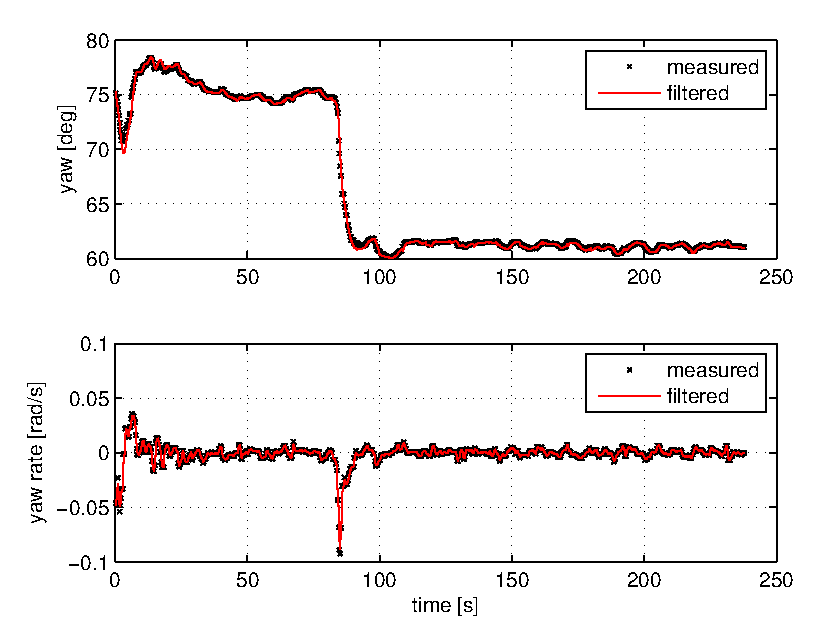
\includegraphics[width=0.48\linewidth]{simulations/fig/yaw-straight2.eps}} \\   
\caption{AUV localisation using EKF with high confidence in yaw measurement, SDyaw = 0.01$rad \approx 0.6 ^{\circ}$. SDyawRate = 0.004 $\frac{rad}{s}$, SDu/v = $1\frac{cm}{s}$.}

\label{fig:auv-sim-straight2}
\end{figure}
\begin{figure}%[htb]
  \centering
    \subfigure[N/E localisation. Yaw was calculated by integrating yaw rate periodically measured using FOG.] {\label{fig:sim-straight1}
	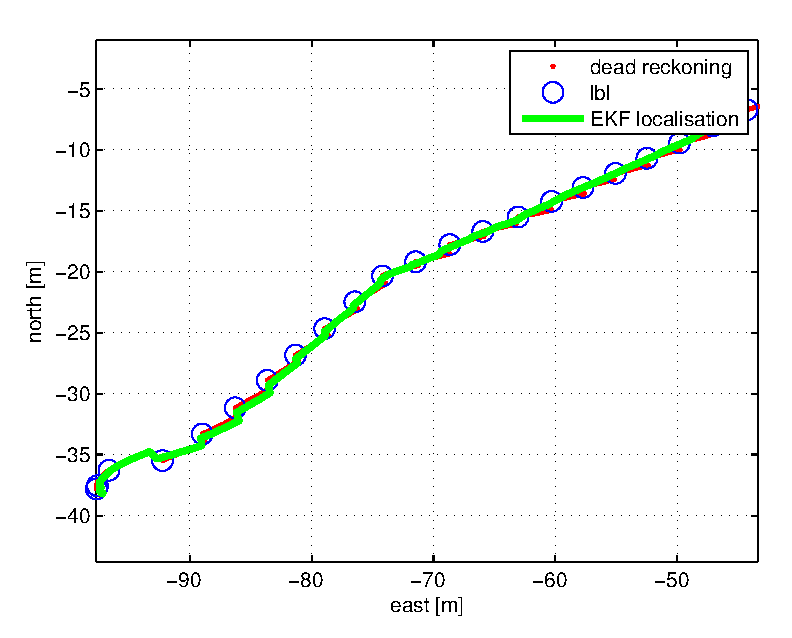
\includegraphics[width=0.48\linewidth]{simulations/fig/sim-straight1.eps}}
    \subfigure[Heading estimation. Biased yaw measurement is being corrected.] {\label{fig:yaw-straight1}
    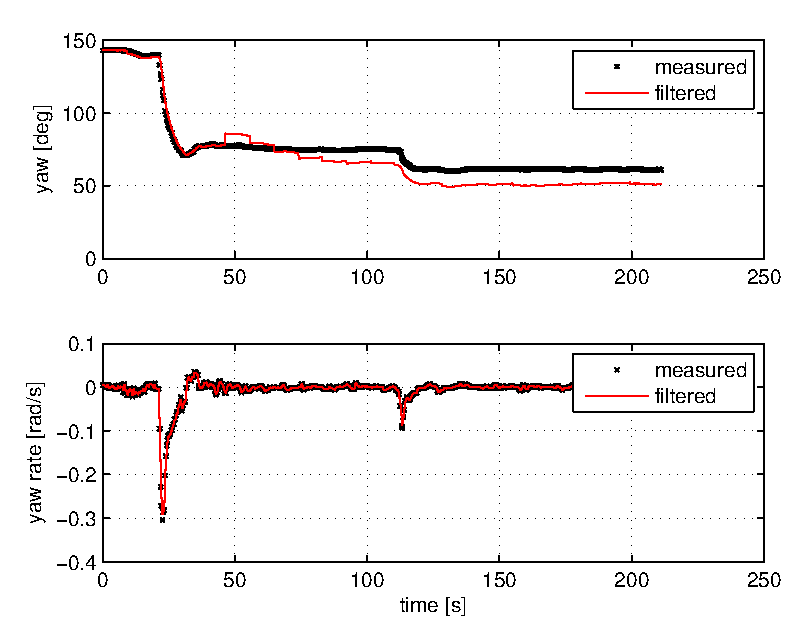
\includegraphics[width=0.48\linewidth]{simulations/fig/yaw-straight1.eps}} \\
\caption{AUV localisation using EKF with low confidence in yaw measurement, SDyaw = 0.2$rad \approx 11.5 ^{\circ}$. SDyawRate = 0.004 $\frac{rad}{s}$, SDu/v = $1\frac{cm}{s}$.}
%\vspace{-10pt}
\label{fig:auv-sim-straight1}
\end{figure}    
%After  initial heading, yaw rate was integrated in time to calculate yaw.    when setting  EKF parameter uncertainty  when using EKF, this time
EKF updates periodically (synchronous mode), with period set to 230 ms. At first, simulation parameters \textit{SDnorth}, \textit{SDeast}, \textit{SDyaw} and \textit{SDyawRate} were set to low values - suggesting high trust in measurements. Resulting trajectory (Figure ~\ref{fig:sim-straight2}) shows that the heading measurement has a constant bias, caused by the error in initial heading measurement obtained by compass. Thus, yaw measurement, calculated relative to previous value each time, propagates the error (bias). Biased yaw observation further on causes EKF localisation to experience sharp jumps. To overcome this using EKF framework, less confidence was assigned to the yaw measurement (\textit{SDyaw}) value. Eventually, bias becomes visible if measured and filtered heading are compared (Figure ~\ref{fig:yaw-straight1}). As for the rest of the heading information, rate of yaw measurement will be incorporated with a lot of confidence (\textit{SDyawRate} parameter having range of degrees) since it is a reliable device and it does not depend on the initial estimate. Good feature of sensor fusion is that lack of one measurement or its low performance can be compensated with some other measurement considering that they are combined together in mathematical model in the right manner. In case of yaw and yaw rate - the derivation in time is a relation that connects them together. 

Simulation shows that localisation performance can be tailored by setting the confidence in prediction model or measurement values. Confidence is materialized as standard deviation (variance) of the random variable: the lower it is, more certain the value of the random variable is hence more confident in value of that variable we tend to be. Kalman filter tries to optimise the result within the defined boundaries of uncertainty. 

Unscented Kalman filter was mentioned in Section \S~\ref{sec:ukf} as a good alternative in handling nonlinearities. UKF was implemented in MATLAB for the simulation purposes and its result compared with the EKF localisation, under same parameter settings and using the real data obtained from Nessie sensors. Test mission consisted of pipe tracking where the vehicle was guided along the underwater pipe three times and each time returned back to the initial position (Figure ~\ref{fig:ekf-ukf}). 2D north-east maps were compared, together with dead reckoning, same as one used for previous simulations. General characteristics of UKF are visible from the obtained shape of the UKF path (Figure ~\ref{fig:ekf-ukf}). Eventually, both filtered paths end up in approximately same position, having less drift than the dead reckoning. EKF does first order approximations, therefore, its path is slightly distorted compared with the UKF one, which was obtained with the same amount of calculation, and the inherited approximation of at least second order \cite{julier96}. Simultaneously with filtering, UKF preserves the nonlinearity formula of prediction model better - its curves have shape closer to equation-based dead reckoning curves. Still, a question that is yet opened is whether we need to improve the approximation of the prediction model. Answering this question is a hard task without knowing the movement of the object and how much it actually matches the state prediction model. A difficulty with UKF implementation is that it involves calculation of covariance matrix square root which is a slightly more complex problem, solved with numerical methods. Nevertheless, it is possible that covariance matrix becomes singular which also depends on parameter $k$ used for scaling (Section \S~\ref{sec:ukf}). $k$ was set to -0.5 for simulations shown.        
\begin{figure}%[htb]
  \centering
    \subfigure[N/E localisation. Comparison of the EKF and UKF.] {\label{fig:ekf-ukf}
	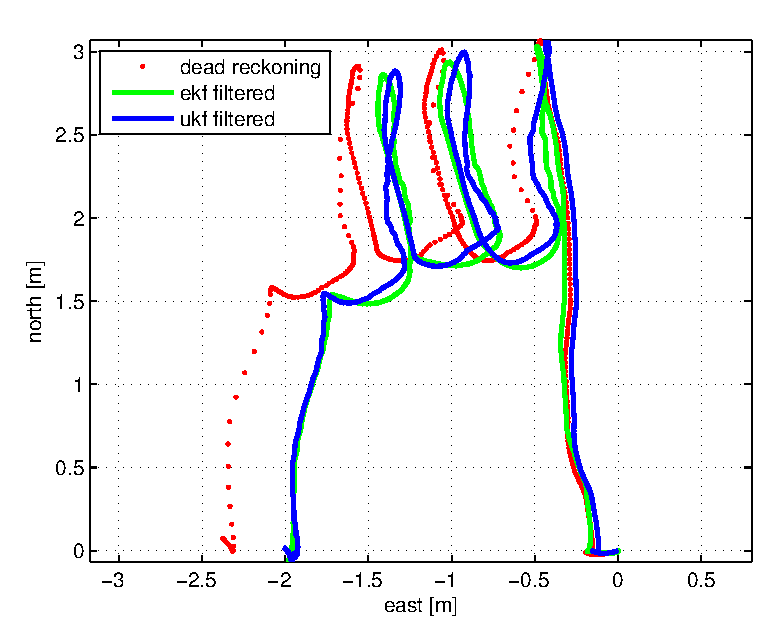
\includegraphics[width=0.42\linewidth]{simulations/fig/UKFpipeTrack.eps}}
    \subfigure[Magnetic disturbances affecting the heading measurement by compass. Vehicle is not moving, FOG is not oscillating at the same time.] {\label{fig:magnetic-disturb}
    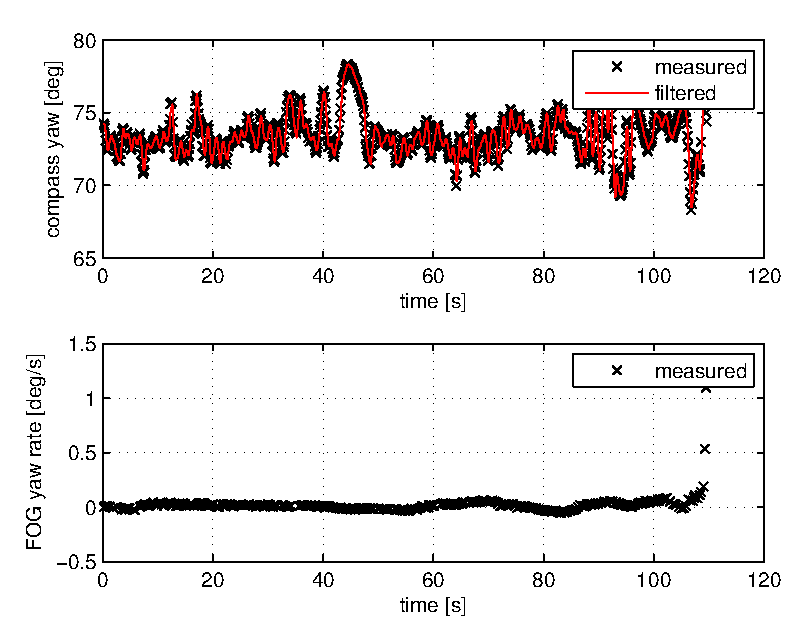
\includegraphics[width=0.42\linewidth]{simulations/fig/magnetic.eps}} 
%\vspace{-33pt}  
\end{figure}

\T{Sensor fusion for heading: } being in search for heading measurement less prone to initial error, and guided by simulation results, real scenarios were accomplished using magnetic compass for heading measurement. Compass is more sensitive to magnetic disturbances (Figure ~\ref{fig:magnetic-disturb}), slower than FOG but, importantly, gives an absolute measure. Therefore, it does not rely on previous measurements. An experiment was made by just manually rotating the robot horizontally while keeping the same position - changing its heading. Figures ~\ref{fig:lostFog} and ~\ref{fig:lostCompass} show the performance of yaw filtering using EKF and the example of sensor fusion of compass and FOG. Namely, compass (Figure ~\ref{fig:lostCompass}) or FOG (Figure ~\ref{fig:lostFog}) were disabled at one point during the experiment. When one of them stops working, the other one tries to compensate the failure. 
%and still filters the heading/yaw rate variation.  
\begin{figure}%[htb]
  \centering
    \subfigure[Compass disabled.] {\label{fig:lostCompass}
	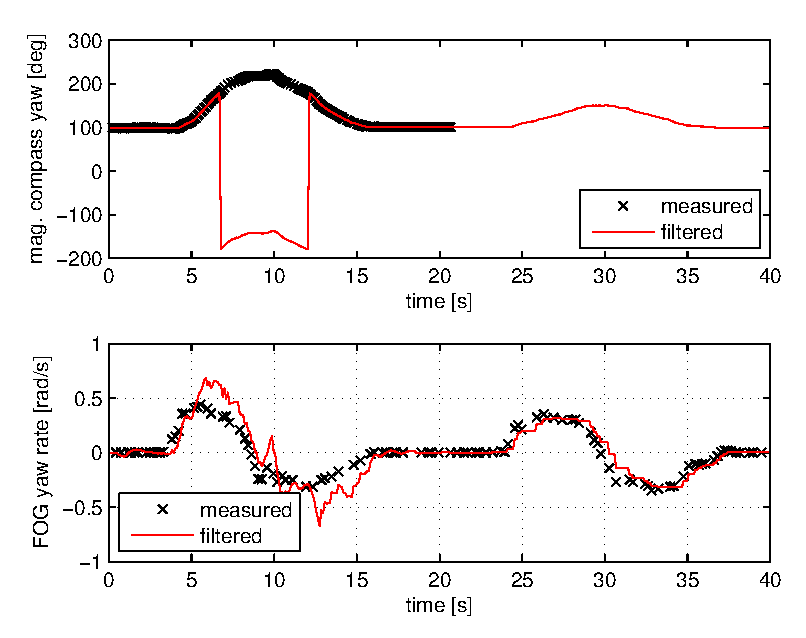
\includegraphics[width=0.45\linewidth]{results/fig/lostCompass.eps}}
    \subfigure[FOG disabled.] {\label{fig:lostFog}
    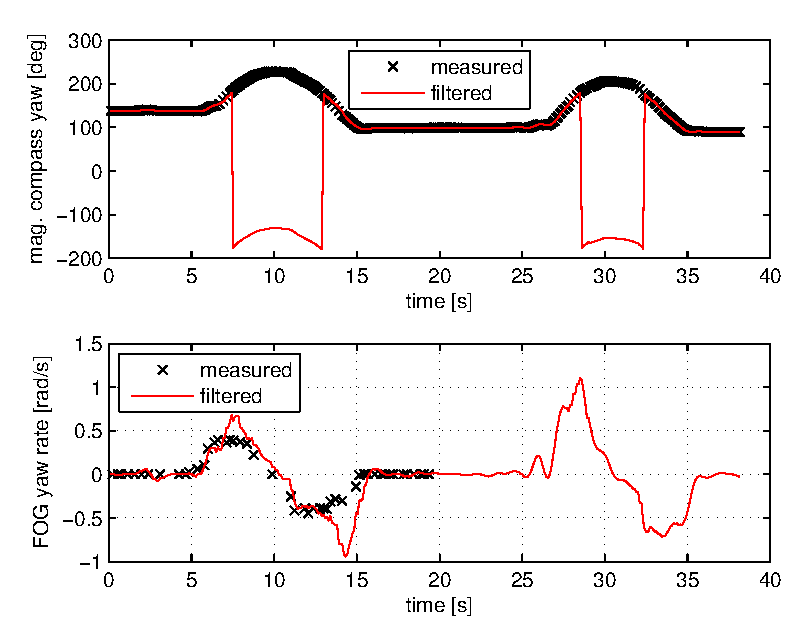
\includegraphics[width=0.45\linewidth]{results/fig/lostFOG.eps}} \\   
\end{figure}

\T{Trajectory filtering: } Spiral trajectory and surfacing action was taken with Nessie starting from the depth of around 12 m. EKF filtering results are shown in Figure ~\ref{fig:spiral} together with LBL position updates and dead reckoning starting from each position. Similarly as with previous plots, dead reckoning was shown together with LBL position updates. Filtered trajectory does not experience severe jumps, and the curve seems to be smoother and less prone to drifting. Standard deviation of north and east measurement parameter (Table ~\ref{tab:ekf-params}) was tested with different values, causing more or less confidence in LBL measurement hence shaping the filtered localisation curve. Presented LBL measurements are exhibiting quite diverse range of values.

Causes of position correction errors are numerous: from ``multipathing'' outliers (Figure ~\ref{fig:multipathing}) till the imprecision inferred from the nature of volatile acoustic and GPS information. ``Multipathing'' causes outliers in position information as a result of false reflections for instance. Acoustic and GPS imprecision can be treated as Gaussian random variable. 
\begin{wrapfigure}{r}{0.55\textwidth}
\vspace{-10pt}
  \centering
    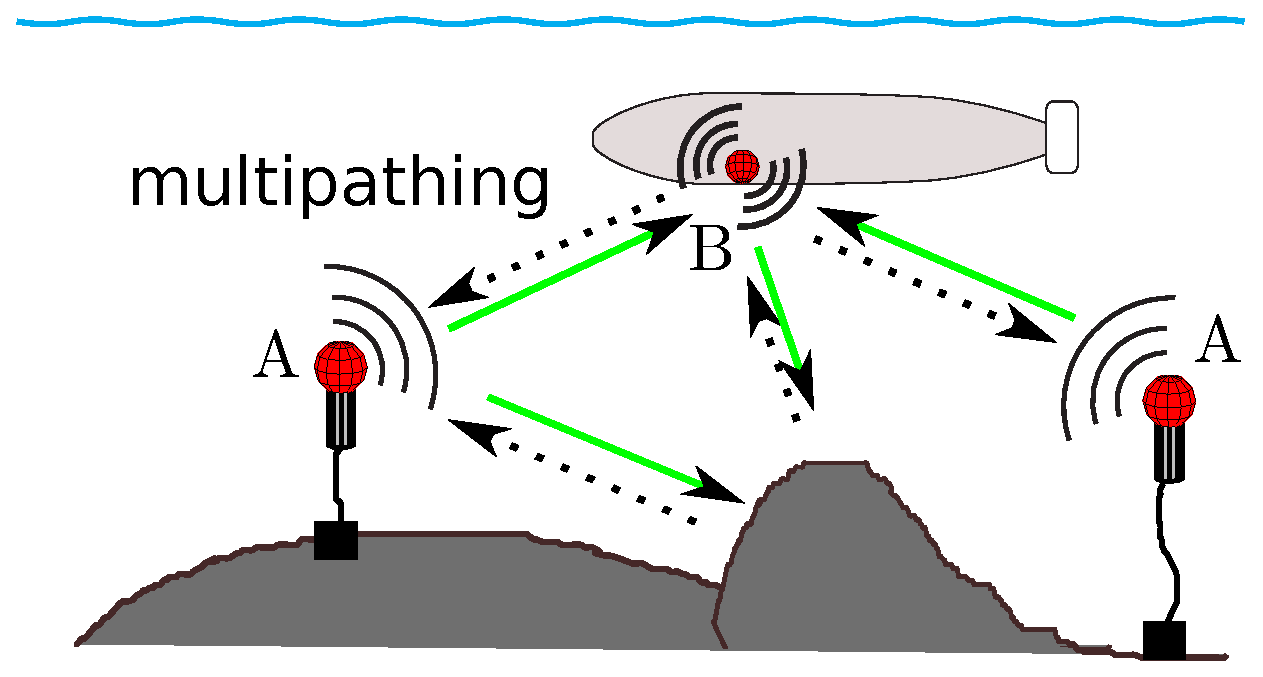
\includegraphics[width=0.45\textwidth]{results/fig/multipathing.eps}
  \caption{Multipathing can cause outliers in LBL position measurement. Due to reflection, several distances are detected, some  being false measurements.}
%\vspace{-10pt} 
\label{fig:multipathing}
\end{wrapfigure}
It is likely that some of the LBL position updates deviate from the trajectory. Hence, a mechanism for rejecting the outliers was investigated. EKF was tested on raw LBL position updates. Intention is to manage the filtration of the ``outliers'' by using properly tuned EKF. Motivation to explore such possibility comes from two scenarios encountered in earlier missions. In such missions position wad dead reckoned and LBL was used to assign each time a new value of north and east coordinate. LBL outliers were ruled out using a median filter applied on the last eleven position coordinates once the latest LBL exceeded the set threshold in position change. The missions showcased situations when: 
\begin{itemize}
\item LBL rejection is carried out despite being a ``false alarm'' - Figure ~\ref{fig:straight-median-ekf},
\item rejection of the LBL is the right choice - Figure ~\ref{fig:spiral-median-ekf}
\end{itemize}
It is important to say that LBL position filtering was implemented in form of median filter. EKF was updated with raw LBL data instead of median filter. Rejecting an LBL measurement can turn out to be right (Figure ~\ref{fig:spiral-median-ekf}) as well as a wrong decision (Figure ~\ref{fig:straight-median-ekf}). That is why EKF was suggested as an alternative. Examples of EKF's performance are shown in both Figures ~\ref{fig:straight-median-ekf} and ~\ref{fig:spiral-median-ekf}. Solution is not as categoric as median filter. Moreover, it is more robust. By giving certain trust in LBL observation it always takes it into account. Median filter, on the other hand, can be too selective in being right or wrong. If it turns out that LBL positions do follow each other, EKF continues slowly following that direction. If the outliers are isolated, EKF successfully rules them out (Figure ~\ref{fig:spiral-median-ekf}). 
\begin{figure}%[htb]
  \centering
    \subfigure[Straight trajectory: LBL outliers erroneously rejected (red). EKF tends to recover the navigation (green).] {\label{fig:straight-median-ekf}
	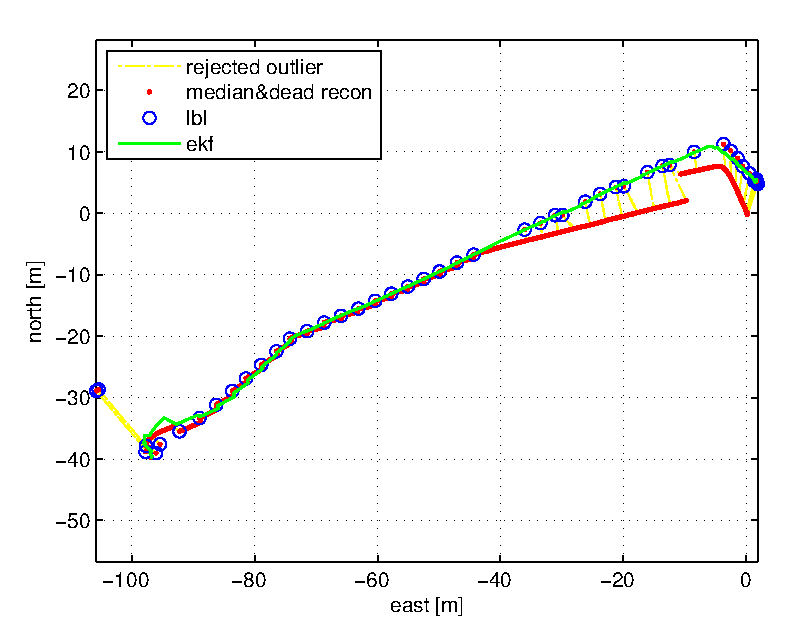
\includegraphics[width=0.47\linewidth]{results/fig/straight-median-ekf.eps}}
    %\subfigure[Straight trajectory: LBL outliers filtered with EKF.] {\label{fig:straight-ekf}
    %\includegraphics[width=0.45\linewidth]{results/fig/straight-ekf.eps}} \\  
    \subfigure[Spiral trajectory: LBL outliers are rejected using median. EKF filtering introduces the position disturbance which recovers soon after.] {\label{fig:spiral-median-ekf}
    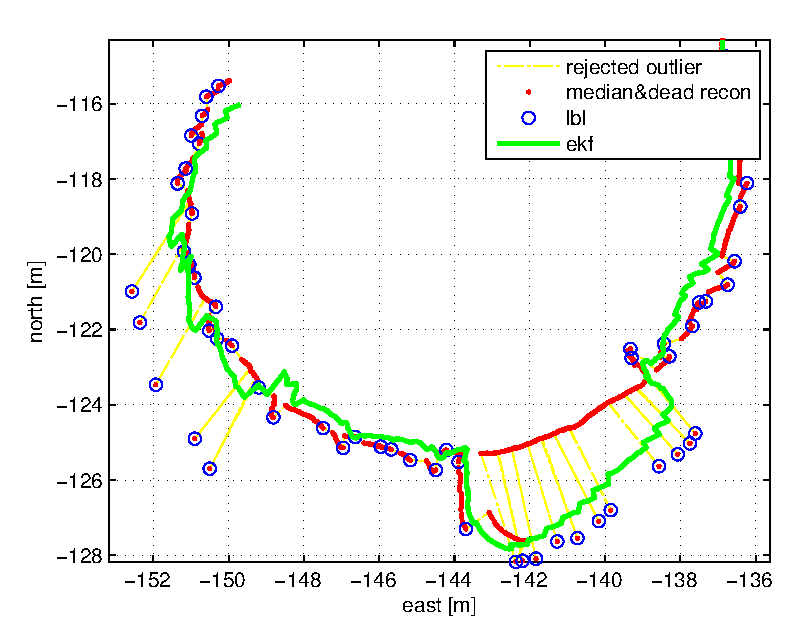
\includegraphics[width=0.5\linewidth]{results/fig/spiral-median-ekf.eps}} 
    %\subfigure[Spiral trajectory: LBL outliers filtered with EKF.] {\label{fig:spiral-ekf}
    %\includegraphics[width=0.45\linewidth]{results/fig/spiral-ekf.eps}}     
\end{figure}

\T{Square trajectories: } square trajectories were tested in low depths of a lake, with the GPS signal available to be used as a position reference and ground truth indication (Figures ~\ref{fig:no-gps}, ~\ref{fig:with-gps}). Dead reckoning navigation was used as a reference when controlling the vehicle movement during the experiment. This fact can cause slight confusion in analysis of the trajectory graphs since all the dynamics and forces were applied with respect to the dead reckoning navigation which is an estimated value, not the real existing one. It is a slightly inverse logic of testing, nevertheless further tests are yet to be accomplished. Emphasis of this experiment was to show that EKF can work successfully and analyse the main characteristics of the navigation design. It is likely that the GPS emulated square-shaped trajectories float as the elapsed path becomes longer. GPS signal available from the antenna located on the water surface is serving as a measure of absolute position within the lake - giving an idea about the actual vehicle position while it tries to moves within the boundaries of estimated dead reckoning position. 

Main issue when performing the square trajectory tests was significant imprecision of GPS signal. Many reasons can possibly influence the imprecision: from the weather conditions till surrounding objects. Basically anything that can affect the satellite visibility and the quality of the signal. Drifting can reach up to several meters which is unacceptable considering the trajectory length. Finally, the trajectory of the experiment itself is quite short ($ \approx 10 m $) to be seriously and accurately covered with precise GPS position update. Figure ~\ref{fig:gps} shows the tested trajectory and depicts the encountered amount of GPS imprecision.
\begin{figure}%[htb]
  \centering
    \subfigure[Coordinates of the tested square trajectory pasted on the lake map.] {\label{fig:gps-map}
	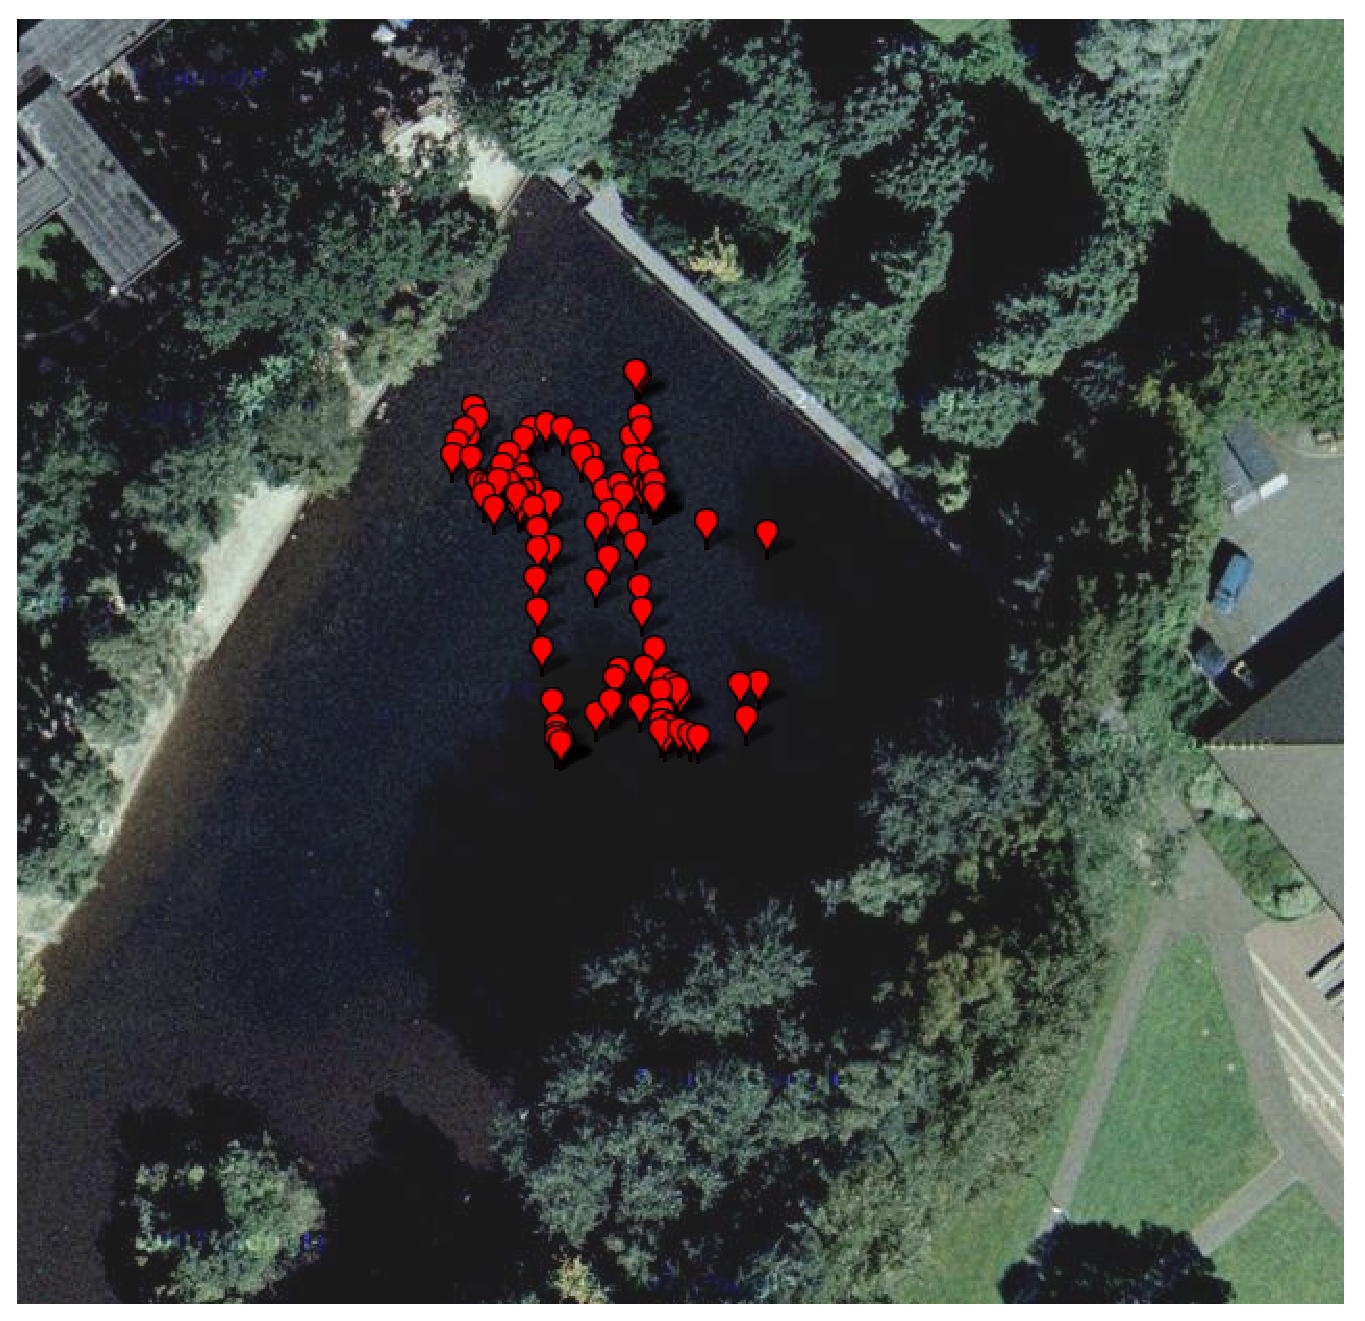
\includegraphics[width=0.48\linewidth]{results/fig/square-trajectory.eps}}
    \subfigure[GPS signal as it appears originally.] {\label{fig:gps-signal}
	\includegraphics[width=0.48\linewidth]{results/fig/gps-signal.eps}}
\end{figure}

\T{Without GPS: } EKF localisation was tested in given conditions. Initially, only motion (inertial) sensors were used within the observations. That implies all the available linear and angular velocity sensors. Absolute position (raw GPS signal in this constellation) was not included in observations. EKF periodically updates (synchronous mode, \S~\ref{chap:methodology}), with the rate of 10 Hz. The aim was to measure the performance and the amount of drifting that occurs since the robot is intended to repeatedly attain square-like paths and return to the starting position in ideal scenario. It is useful to mention that proper parameter tuning can significantly change filtering performance. By giving more or less trust in particular measurement, or particular model behaviour, the role of certain parameters of dynamics (velocities, angular velocities) can be emphasized if necessary. Figure ~\ref{fig:no-gps} shows the performance of EKF without GPS position correction after one trajectory cycle, and the original path that was followed, recorded using GPS. Initial position was taken from the first GPS measurement and the first measurement can indeed be away from the real position due to GPS imprecision. Note that the control of the vehicle trajectory refers to dead-reckoning calculated north-east values, not some physical beacons with known position. At the time of reporting the experiments, testing were not fully completed with all the planned scenario variations. Localisation expectedly tends to perform with a significant drift without the absolute position update (Figure ~\ref{fig:square-1-noGps}). After the second square-shaped cycle (Figure ~\ref{fig:square-2-noGps}), EKF shows that it roughly tracks the shape of the trajectory, smooths it by filtering out the measurement outliers. Vehicle has returned approximately to the same position after each cycle. Drift gained when following one of the sides of the rectangular path was compensated with the same amount of drift but of the opposite sign that was active when taking the return direction. Enormous amount of drift is present since the information on absolute position is not considered. The first available GPS coordinate fixes the starting position and part of the initial position error is caused by being incapable of setting the initial position accurately.       
\begin{figure}%[htb]
  \centering
    \subfigure[N/E localisation.] {\label{fig:spiral2d}
	\includegraphics[width=0.48\linewidth]{results/fig/spiral2d.eps}}
    \subfigure[Depth.] {\label{fig:spiral-depth}
    \includegraphics[width=0.48\linewidth]{results/fig/spiral-depth.eps}}
    % \\  
    %\subfigure[Path (temporary plot).] {\label{fig:spiral3d}
    %\includegraphics[width=0.8\linewidth]{results/fig/spiral3d.eps}} 
\end{figure}
\begin{figure}%[h]
  \centering
    \subfigure[EKF localisation after one cycle.] {\label{fig:square-1-noGps}
	\includegraphics[width=0.48\linewidth]{results/fig/square1NoGps.eps}}
    \subfigure[EKF localisation after two cycles.] {\label{fig:square-2-noGps}
	\includegraphics[width=0.48\linewidth]{results/fig/square2NoGps.eps}}\\
    %\subfigure[] {}
    %\includegraphics[width=0.6\linewidth]{results/fig/dynamics.eps}}
    \caption{EKF localisation using only inertial measurements as observation.}
    \label{fig:no-gps}
\end{figure}

\begin{figure}%[hb]%tb
  \centering
    \subfigure[Setting standard deviation of 1 m in uncertainty position observation (SDnorth = SDeast = 1.0 m).] {\label{fig:square-withGps-1}
	\includegraphics[width=0.48\linewidth]{results/fig/squareWithGps-10.eps}}
    \subfigure[EKF localisation after tuning the position uncertainty (SDnorth = SDeast = 0.5 m).] {\label{fig:square-withGps-2}
	\includegraphics[width=0.48\linewidth]{results/fig/squareWithGps-05.eps}}
    %\\
    %\subfigure[Linear and angular velocities during square-shaped trajectory.] {\label{fig:square-dynamics}
    %\includegraphics[width=0.45\linewidth]{results/fig/dynamics.eps}}
    \caption{EKF localisation aided with GPS position updates weighted by setting appropriate parameters.}
    \label{fig:with-gps}
\end{figure}
\begin{figure}
\centering
\includegraphics[width=0.6\linewidth]{results/fig/dynamics.eps}
\caption{Linear and angular velocities during square-shaped trajectory.}
\label{fig:square-dynamics}
\end{figure}
\T{With GPS: } Finally, GPS measurements were appended to the EKF observations. Localisation results were shown in Figure ~\ref{fig:with-gps} for two different level of confidence (variances) in position measurement. Naturally, giving extremely high confidence does not seem to be the best choice, however, some empirically deduced values in range of decimetres significantly correct the dead reckoning drift. Furthermore, EKF tends to filter the GPS measured north east coordinates, hence partially corrects the GPS imprecisions stated at the beginning. At this point it is evident why EKF is a great tool. Filter tries to satisfy the set uncertainty boundaries and fuse all the available information trying to make the most out of it combined together in one mathematical system. Moreover, fusing such imprecise and sketchy position data from GPS, still improves the localisation. Obtained trajectory tends to go towards what can be treated as expected path. From something that looked like a noisy collection of position observations at the beginning (Figure ~\ref{fig:gps-signal}), application of EKF together with sensor fusion enabled having generally better performance in navigation.     
%Combination of all relevant sensors gives in a Kalman filter state estimate results in more precise position and heading compared with instant (flat) usage of position and orientation measurements.  
%\subsection{Sensor selection}
%Design and performance test.
%\subsection{Using FOG for navigation improvement}
%How big is the improvement with respect to the distance travelled?


%%%%%%%%%%%%%%%%%%%%%%%%%%%%%%%%%%%%%%%%%%%%%%%%%%%%%%%%%%%%%%%%%%%%%%%%%%%%%%%
%\begin{frame}[fragile] % Notice the [fragile] option beside \begin{frame} %
%\frametitle{Verbatim}
%\begin{example}[Putting Verbatim]
%\begin{verbatim}
%\begin{frame}
%\frametitle{Outline}
%\begin{block}
%{Why Beamer?}
%Does anybody need an introduction to Beamer?
%I don't think so.
%\end{block}
%\end{frame}\end{verbatim} % Extra carriage return causes problem wit verbatim %
%\end{example}
%\end{frame}

%%%\begin{frame}[fragile]  % notice the fragile ooption, since the body
%%%			% contains a verbatim command
%%%Example of the \verb|\cite| command to give a reference is below:
%%%
%%%With an example of citation, \cite{ribas10}, we may proceed to the Bibliograhy section.
%%%\end{frame}

\begin{frame}
\frametitle{References}
\footnotesize{
\begin{thebibliography}{99}

%      \bibitem{ribas10} 
%      D. Ribas, P. Ridao, and J. Neira.
%      \newblock {U}nderwater {S}lam for {S}tructured {E}nvironments using an {I}maging {S}onar
%      \newblock {\em Springer Verlag, 2010}

 \bibitem{ribas10} D. Ribas, P. Ridao, and J. Neira. (2010)
 \newblock {U}nderwater {S}lam for {S}tructured {E}nvironments using an {I}maging {S}onar. \newblock \emph{\em Springer Verlag} 
%  
 
 \bibitem{julier96} Julier, S. and Uhlmann, J.K. (1996)
 \newblock {A} general method for approximating nonlinear transformations of probability distributions.
 \newblock \emph{\em Robotics Research Group, Department of Engineering Science, University of Oxford}
 
 \bibitem{thrun05}  S. Thrun, W. Burgard, and D. Fox. (2005)
 \newblock {P}robabilistic robotics
 \newblock {\em MIT Press}	
 
 \bibitem{grewal01} Grewal, M.S. and Andrews, A.P. (2001)
 \newblock {K}alman filtering: theory and practice using MATLAB.
 \newblock {\em Wiley Online Library}
  
 \bibitem{ristic04} Ristic, B. and Arulampalam, S. and Gordon, N. (2004)
 \newblock {B}eyond the Kalman filter: Particle filters for tracking applications.
 \newblock {\em Artech House Publishers}

% \bibitem{farrell98} Jay Farrell and Jay A. Farrell (1998)
% \newblock {T}he Global Positioning System \& Inertial Navigation.
% \newblock {\em McGraw-Hill Professional} 
       
\end{thebibliography}
}
\end{frame}

\begin{frame}
\centerline{The End}
\end{frame}


% End of slides
\end{document} 